\pdfoutput=1
\documentclass[11pt,reqno]{amsart}

\usepackage[utf8]{inputenc}
\usepackage[T1]{fontenc}
% U+2212 (minus sign) reaches the bibliography through biber when a title
% carries a Unicode superscript minus; pdflatex has no default mapping for it.
\DeclareUnicodeCharacter{2212}{-}
\usepackage[margin=1in]{geometry}
\usepackage{mathtools}
\usepackage{amsmath,amssymb,amsthm}
\usepackage{booktabs}
\usepackage{array}
\usepackage{graphicx}
\graphicspath{{images/}}
\usepackage{float}
\usepackage{xcolor}\definecolor{linkred}{rgb}{0.78,0.08,0.12}
\usepackage[backend=biber,style=numeric,sorting=nyt,giveninits=true,doi=true,url=true,isbn=false]{biblatex}
\addbibresource{src/bibliography.bib}
\AtEveryBibitem{\iffieldundef{doi}{}{\clearfield{url}}}
\usepackage{hyperref}
\hypersetup{colorlinks=true,urlcolor=blue,linkcolor=linkred,citecolor=blue}

\newcommand{\golden}{\varphi}
% draft marker of the author's manuscript (v134); unused in the text, kept for fidelity
\newcommand{\pending}[1]{{\color{red}[#1]}}
% ---------------------------------------------------------------------------
% Witness system.  Colour by class; a mark with ids stays inline \tier[ids]{X}
% and moves to a line of its own in list form, P[name1, name2], when the gates
% of docs/citations.md section 8.5 hold: two ids or more at 35 characters or
% more, the mark closing its sentence (r = 0), not closing a list item (i = 0),
% and standing 75 words or more from the nearest witness block of its
% blank-line paragraph (d >= 75).  Two heuristics sit between those gates in
% the decision order - u, the shape of the run of marks a list already has, and
% p, a mark at the close of its paragraph - both labelled in section 8.5.
% Every mark selects its own font with \normalfont..., so neither an enclosing
% \itshape (amsthm's plain theorem style) nor an open \emph can leak into it.
% ---------------------------------------------------------------------------
\definecolor{tierP}{rgb}{0.15,0.35,0.65}   % blue   -- proved in Lean
\definecolor{tierPs}{rgb}{0.70,0.45,0.05}  % ochre  -- written in Lean, no name cited
\definecolor{tierN}{rgb}{0.05,0.40,0.20}   % green  -- verified numerically
\definecolor{tierW}{rgb}{0.00,0.35,0.45}   % teal   -- witness item
% allow line breaks after underscores, commas and dots inside code names
\makeatletter
\DeclareRobustCommand{\brk@us}{\textunderscore\allowbreak}
\newcommand{\code}[1]{{\upshape\ttfamily\let\_\brk@us #1}}
% the test that checks a number, cited by its pytest name; the argument is
% written with \_ so a long name can break across lines, and
% tests/test_section_census.py requires every one of them to exist
\newcommand{\testref}[1]{{\upshape\small\ttfamily\let\_\brk@us #1}}
\@namedef{tiercol@P}{\color{tierP}}
% internal/protected: draft-stage marker between builds; functional and rendering, but not used in the final/release text
\@namedef{tiercol@P*}{\color{tierPs}}
\@namedef{tiercol@N}{\color{tierN}}
\@namedef{tiercol@W}{\color{tierW}}
\newcommand{\tiercol}[1]{\expandafter\ifx\csname tiercol@#1\endcsname\relax\else\csname tiercol@#1\endcsname\fi}
% inline status tag: [P], [N] ... unbreakable, its own colour and its own
% style.  One macro, one optional argument, one grammar; the tag always
% comes first and its reference inside the brackets:
%   \tier{X}              -> [X]   the witness lives in the prose of the
%                                  same sentence (a \testref, the name of
%                                  one of our Lean declarations, an
%                                  \eqref/\ref or a \witness);
%   \tier[ids]{X}         -> X[ids] the optional argument carries INTERNAL
%                                  ids only -- a \testref, or the names of
%                                  declarations of our own Lean file, which
%                                  are written raw (no macro around them)
%                                  and print in tt inside the tag's own
%                                  brackets, several of them separated by
%                                  ','.  An external source is never a key
%                                  of the tag: it is a real \cite set next
%                                  to the tag ([N]~\cite{key}, [P]
%                                  in~\cite{key}), so a tag never prints a
%                                  number in its bracket.
%   a citation key in the optional argument (a plain alnum token: no \_,
%   no comma, no \testref) is an error, not a fallback
\def\tier@inside#1#2{{\normalfont\footnotesize\bfseries\tiercol{#2}#2[#1]}}
% raw internal names: the bracket is set in tt, with breakable underscores
\def\tier@names#1#2{{\normalfont\footnotesize\bfseries\tiercol{#2}#2[{\upshape\small\ttfamily\let\_\brk@us #1}]}}
\providecommand{\tier}[2][]{%
\ifx\relax#1\relax
{\normalfont\footnotesize\bfseries\tiercol{#2}[#2]}%
\else
\in@{\testref}{#1}\ifin@
\tier@inside{#1}{#2}%
\else
\in@{\_}{#1}\ifin@
\tier@names{#1}{#2}%
\else
\in@{,}{#1}\ifin@
\tier@names{#1}{#2}%
\else
\PackageError{tier}{the optional argument of \string\tier\space holds internal ids only}
{An external source is a \string\cite\space set next to the tag, never its key; a name of our own Lean file is written raw, with \string\_.}%
\fi\fi\fi
\fi}
% a witness with names, on a line of its own, flush right: P[name1, name2]
% (the sibling manuscripts set their witness blocks with \hfill + \raggedleft,
% see \ProofWitnessBlock in 03-crystalline-worldsheet)
\newcommand{\witness}[2]{%
  \par\noindent\hfill
  \parbox{\dimexpr\linewidth-1em\relax}{\raggedleft
    \normalfont\footnotesize\bfseries\tiercol{#1}#1\mdseries{\upshape\small\ttfamily\let\_\brk@us[#2]}}%
  \par}
% witness label of the W list: W1[CLPW]
\newcommand{\wtag}[2]{{\normalfont\footnotesize\bfseries\tiercol{W}#1\mdseries{\small\ttfamily[#2]}}}
\makeatother
\setlength{\emergencystretch}{2em}


\numberwithin{equation}{section}

\newtheorem{theorem}{Theorem}[section]
\newtheorem{proposition}[theorem]{Proposition}
\newtheorem{corollary}[theorem]{Corollary}
\newtheorem{definition}[theorem]{Definition}
\theoremstyle{remark}
\newtheorem{remark}[theorem]{Remark}
\newtheorem{imported}{Imported statement}
\renewcommand{\theimported}{I\arabic{imported}}

\title[One object instead of a choice of vacuum]{\textbf{One object instead of a choice of vacuum\\to put the observer in de~Sitter space}\\[2pt]
From wormholes, black holes and baby universes\\to the criteria for an observer in de~Sitter,\\contrasted with the Kaluza--Klein graviton candidates\\and with the cosmological constant}
% amsart prints the \address/\email blocks from \enddoc@text, i.e. at the end
% of the document (amsart.cls: \AtEndDocument{\enddoc@text}); that is the
% placement the author chose, kept as the class default.  The byline follows
% the manuscript (Gonzalez, Gonzalez, Dressler, Garcia), so the institutional
% address is declared twice -- once for each group that carries it -- and the
% three institutional e-mail addresses are listed together with the first
% group; the independent author keeps her own address and e-mail.
\author[J. A. González García et al.]{J.~A.~Gonz\'alez Garc\'ia}
\author[]{V.~M.~Gonz\'alez Garc\'ia}
\address{TTAMAYO PUNTO COM, S.A.P.I.\ de C.V.; Research \& Development Division;
  Naucalpan de Juárez, State of Mexico, Mexico}
\email{jorge@ttamayo.com, victor@ttamayo.com, luz@ttamayo.com}
\author[]{I.~M.~Dressler P\'erez}
\address{Independent Researcher}
\email{itzel@omega-pcf.com}
\author[]{L.~M.~Garc\'ia Ord\'o\~nez}
\address{TTAMAYO PUNTO COM, S.A.P.I.\ de C.V.; Research \& Development Division;
  Naucalpan de Juárez, State of Mexico, Mexico}
\renewcommand{\datename}{\textbf{Received:}}
% Received date, last-modified date and version, with the labels in bold.
% amsart prints \date as the footnote at the foot of page 1 (\@adminfootnotes
% -> \@setdate, which prefixes \datename), so the first label lives in
% \datename and the line carries the other two: without this the class would
% prefix its own "Date:" and the footnote would read "Date: Received: ...".
% \today is reproducible:
% scripts/tasks/compile.ts compiles with SOURCE_DATE_EPOCH set to the HEAD
% commit's timestamp, so it prints the date of the last commit, never the
% clock's.  The version token is owned by package.json: the "version"
% markers below are checked by `pnpm run selfcitations:check` (in
% `pnpm run validate`), which fails when this line and package.json differ,
% and rewritten by `pnpm run selfcitations` / `pnpm run build`.
% selfcite:begin id="version"
\date{November 16, 2026; \textbf{Last modified:} \today; \textbf{Version:} \texttt{v0.1.0}}
% selfcite:end id="version"

% The counts this note asserts are MEASURED, never typed: `pnpm run counts`
% (scripts/tasks/counts.ts) rewrites the block below and the prose regions
% marked `counts:begin` — they quote its macros — `pnpm run counts:check`
% fails with a diff on any drift, and `pnpm run build` re-syncs both before
% the render, so the PDF prints the measured value.
% counts:begin id="macros"
\newcommand{\CountSections}{47}
\newcommand{\CountTests}{498}
\newcommand{\CountNotSlow}{495}
\newcommand{\CountTheorems}{164}
\newcommand{\CountAxioms}{6}
\newcommand{\CountSorry}{0}
% counts:end id="macros"

\begin{document}

\begin{abstract}
In de~Sitter space an observer must be inside the universe it observes, and in string theory placing
it has become a choice: of a vacuum among some $10^{500}$. The same choice returns where wormholes,
black holes and baby universes meet. The baby universes that branch off through wormholes carry
parameters that fix the constants of nature, the cosmological constant among them, and the same
parameters label the boundary theories over which the gravity of a black-hole throat is averaged; in
both the question is which value, and the answer is sought in what a throat contains. The programme
to which this note belongs, written within critical realism, reads the difficulty as one of
representation rather than of selection: what is missing is one object that meets the criteria
Witten and Chandrasekaran, Longo, Penington and Witten set for an observer in de~Sitter, not a
choice among values. This note does not test that claim itself; it tests two of its consequences
where data can reach them, on the particles of one throat and on the cosmological constant. The
object, in the framework of the programme, is a microstate whose levels form a tower built from two
numbers, $\pi$ and the golden ratio $\golden$; read as a warped extra dimension it is a throat, the
golden throat, whose Kaluza--Klein modes are its particles. The question becomes whether the tower
fixes what a throat model otherwise chooses. The two-brane model of Randall and Sundrum assumes the
dimension and chooses the infrared scale and the depth. The golden throat has the same equations, so
the same mass ratios, and four independent conditions of the tower, reflection positivity,
four-dimensional gravity, the arity of the framework and the clock of $\golden$, fix its spectrum
with no free parameter, to leading order $\pi(k+\tfrac14)$ times $M\golden^{12}$ in the unit $M$ of
the framework. The arity gives the dimension that the two-brane model assumes; with $M$ identified
with the scale of the charged leptons and the level $12$ with the bottom of the throat, the spectrum
fixes the infrared scale that it chooses. Identified with the graviton candidates reported at $380$
and $700$~GeV, they place the bottom of the throat at $11.97\pm0.05$, $0.6$ standard deviations from
$12$, and give the next modes at $1028$ and $1346$~GeV, against $1014$ and $1328$~GeV for the
two-brane model fitted to the same candidates. Only the depth, the position of the top, stays free,
and the ratio of the vector modes can decide it if they share its depth, though the gluon candidates place their own bottom at $17.6$--$17.8$. The same tower carries the observer of de~Sitter
space. In the gravitational unit of the framework the observed cosmological constant gives the
observer's level, $583.79\pm0.03$: the level is read from the data, not chosen, and the hypothesis
that it sits at an integer level is excluded within $\Lambda$CDM at $7.6$ standard deviations with DESI and the CMB. What
the note leaves open is one number, the ratio of the lepton scale to the Planck scale.
\end{abstract}

\keywords{de Sitter space, wormholes, Kaluza--Klein gravitons, golden ratio,
Randall--Sundrum model, cosmological constant, formal verification, Lean 4}

\maketitle

\tableofcontents

\section{Introduction}\label{sec:intro}

In de~Sitter space there is no exterior: an observer must be inside the universe it observes and
must be described by the theory~\cite{Wit01,BF01,CLPW23}. In string theory this is the problem of
vacuum selection: among some $10^{500}$ vacua~\cite{BP00} one is chosen in which such an observer can
exist, and beyond the anthropic principle no rule singles it out~\cite{CW6}. The programme to which
this note belongs reads that situation as a problem of representation rather than of selection:
what is missing is a single object that meets the criteria an observer in de~Sitter imposes, not a
choice among vacua~\cite{PRES}.

Those criteria have been stated. Witten asked for a theory that determines the cosmological
constant, with a finite Hilbert space whose dimension is the entropy, a positive pairing, a CPT map
and the antipodal structure of de~Sitter~\cite{Wit01}; Chandrasekaran, Longo, Penington and Witten,
that the observer be described by the theory, with a type~II algebra obtained by crossed product and
a maximally mixed vacuum~\cite{CLPW23}; and Maldacena showed that adding an observer removes the
phase that keeps the sphere partition function from counting states~\cite{Mal24}. Static-patch
holography has been modelled with coupled SYK systems~\cite{Sus21,NV25}, whose two-boundary version is
the eternal traversable wormhole of Maldacena and Qi~\cite{MQ18}, in the $AdS_2$ throat that
Maldacena's conjecture, the meeting point of holography and M-theory, left open~\cite{Mal98}. The
framework of~\cite{CW6} proposes one object, a microstate of modulus $\tfrac12$, that realises the
three von Neumann types the criteria refer to, type~I discrete, type~II of observation and type~III
of the field. The note proves a mathematical signature of each criterion, not the criterion
itself; that the object is the observer's patch is a physical identification.

Where wormholes, black holes and baby universes meet, the word \emph{ensemble} takes two senses,
and both bear on how the observer is placed. Hawking argued that
closed universes branching off a nearly flat region act on its fields as effective interactions that
create or annihilate closed universes containing particles, and read the branching as a loss of
information~\cite{Haw88}, a loss he later argued does not occur~\cite{Haw05}; he also proposed that
black holes may give rise to baby universes~\cite{Haw93}. In third quantization the baby universes are
themselves particles, created and annihilated by a field on superspace~\cite{GS89}, and in
anti-de~Sitter space the states of such wormholes can likewise be read as states containing a given
number of particles~\cite{BG98}. In the model of Marolf and Maxfield the geometry of a black hole is
also the geometry in which baby universes are described: the spacetime wormholes that compute its
entropy link the baby universes to an ensemble of theories, and, keeping the baby universes, each
value of their parameters is a superselection sector that is one theory~\cite{MM20}. From that one
structure the two ensembles follow. In cosmology the parameters fix the constants of nature, the
cosmological constant among them, which Coleman's mechanism drives to zero~\cite{GS88,GS89,Col88}, so
that a value of the parameters plays the part a vacuum plays in the landscape, whose vacua, read with
many worlds, are branches of one wave function~\cite{BS12}. In holography the same parameters label
the boundary theories over which low-dimensional gravity is averaged~\cite{SSS19}, an average that
concerns the microstates of black holes and is not expected below the black-hole
threshold~\cite{SW22}. In three dimensions the average runs over the moduli of the boundary torus~\cite{MW20,ACHT21}. Both ask the same question, which value of the parameters, and both place its
answer in what a throat contains: the throat of the Euclidean wormhole whose section is the baby
universe~\cite{GS88,Col88}, and the $AdS_2$ throat near the horizon of the extremal black
hole~\cite{SSS19}; above three dimensions, if the conjecture of~\cite{MV20} holds, there is only one
sector, and neither ensemble would remain. Holography meets a further choice where its dictionary is made concrete, one that no ensemble removes: a time slice of anti-de~Sitter space is discretised by one regular tiling and a network of tensors of a chosen bond dimension, and the entropy of a boundary region is the number of bonds that its minimal cut crosses times the logarithm of that dimension~\cite{Swi12,PYHP15,JE21}; the tiling and the dimension are chosen, and each tiling fixes its own central charge~\cite{JZE20,BDF20}. Quantum Darwinism gives
another line on how the observer is placed: classical objectivity emerges when the records of a system are redundant in its
environment~\cite{Zur09}, with a threshold and a ceiling in the quantum Fisher
information~\cite{Kie26}. The framework of~\cite{CW6} joins the baby universes and this line. Its observer is a worldline that
accumulates Fisher information up to that ceiling, as the observer of~\cite{CLPW23} is a worldline
carrying a clock; in it each level becomes objective at the threshold $\tfrac12$.

\emph{Evidence tags.} A claim carries its class of evidence in brackets:
\tier{P} proved in Lean~4, machine-checked, with the declaration named in
the bracket; \tier{N} checked numerically, with the test that checks it
named where the check is ours and the citation where the claim is the
literature's. A bracket may hold several witnesses, and a tag on its own
line closes the claim of its paragraph.

That $\tfrac12$ appears three times, proved in~\cite{CW6} and here: the Fisher time
$\tau_F=\tau_D/\sqrt{2f}$ equals the decoherence time $\tau_D$ if and only if $f=\tfrac12$
\tier[fisher\_time\_eq\_decoherence\_iff]{P}, the binary entropy is maximal there, one bit
\tier[bin\_entropy\_half]{P}, and an eigenvalue of modulus $\mu$ carries one bit of Fisher information if and
only if $\mu=\tfrac12$ \tier[fisher\_unit\_iff]{P}. The binary entropy places it at $\tfrac12$ by its symmetry alone, the other two by the constants of their definitions, the $2$ of the Fisher time and the $4$ of the quantum Fisher information, so that they are one fixed point and not three independent conditions. Used in \S\ref{sec:inputs}. That this $\tfrac12$ is the threshold of objectivity
of~\cite{Kie26} is the identification.

The note is written within the paradigm of critical realism~\cite{PRES,Bha75}.
Critical realism distinguishes the objects a science studies, which exist whether or not they are
known, from the theories, models and tools with which it represents them, and it asks of a model
not only whether it is plausible but whether it correctly describes the mechanism at
work~\cite{Bha75}. Read in that way, a construction of this kind has two parts of different kinds,
which must be kept apart: a mathematical structure, whose statements are true or false by proof,
and identifications of its objects with physical ones, which are claims about the world and are
tested by the data. Each identification is named where it is used. A contrast is stated with its criterion before the data are read, with the determination it uses, its worst case and the determinations that would undo it; what holds by construction is said to hold by construction and is not counted as a contrast. In the same tradition,
retroduction is the step from what is found to the structure that makes it possible; the note takes
that step twice, once in mathematics and once in physics. Critical realism has been brought to
quantum theory in peer-reviewed work, but rarely. Mason asks, in the \emph{Journal of Critical
Realism}, whether quantum theory redefines realism on the neo-Copenhagen view~\cite{Mas15};
Elder-Vass uses Bhaskar's realism to bound the ontological conclusions that have been drawn from
quantum mechanics~\cite{EV25}; and Plotnitsky and Khrennikov reach the same question from physics
itself, without starting from critical realism: how far quantum reality can be represented at
all~\cite{PK15}. Few articles join critical realism with quantum mechanics, and, to our knowledge,
none as of 5 November 2026 joins it with quantum gravity, string theory or holography~\cite{REPR}.

The two questions of the baby universes, which value of the parameters, are
questions of selection. The throat of this note is not the throat of the black hole: it is the
five-dimensional throat of the two-brane model~\cite{RS99}, whose particles are its Kaluza--Klein
modes, and its relation to the $AdS_2$ throat is a comparison of form. What the note can test is narrower, two of its consequences: whether, for the particles of one
throat, the parameters that the two-brane model chooses are fixed by one object rather than chosen;
and whether the level that the cosmological constant gives the observer is chosen, fixed or read.

It puts the first to one spectrum, in two parts, one of each kind. The mathematical part:
whether a single operator, built from two numbers, $\pi$ and $\golden$, has a spectrum fixed with no
free parameter. Both numbers are irrational, and each is reached here through a fraction it produces
itself. The physical part: whether that spectrum is the masses of the Kaluza--Klein graviton
candidates reported at the Large Hadron Collider~\cite{LYR26}, which in a warped extra dimension are
the modes of its throat. Why these two numbers is a physical question before it is an arithmetic one. It
is also a question about black holes, read not through an ensemble but through the place of $\golden$
and of the primes in them: the horizon of a distinguished family of extremal Kerr--Newman black holes
is fixed by $\golden$~\cite{SN24}, the interior near a spacelike singularity carries a primon
gas~\cite{Jul90,HY25,DCHY25}, and in $\mathbb Z[\golden]$ whether a prime splits, stays prime or
ramifies is decided by its residue modulo $5$~\cite{Neu99}, the classification of the primes by
$\golden$ that~\cite{GH23,CW6} develop. These relations are the abductions from which the programme
started, not contrasts: from them it built a series of prototypes and found a throat whose warp steps
by $\golden$ and whose modes are spaced by $\pi$, which it proposes as the one object. The throat has two
directions of a different kind. Along the first a mode oscillates: a Kaluza--Klein mode is a standing
wave in the throat, and each successive mode adds half a turn of phase, so the modes are spaced by
$\pi$. This is the angular direction, and its fraction is a quarter-turn: the offset $\tfrac14$ of the
modes, set by the dimension of the slices. Along the second the throat changes scale: in holography
the extra dimension is the energy scale~\cite{SW98}, and moving along it multiplies rather than adds.
A discrete scale without free parameters needs a step, and $\golden$ is the only step for which adding
two levels gives the next, $\golden^{\sigma}+\golden^{\sigma+1}=\golden^{\sigma+2}$, so that the
additive and the multiplicative readings of the tower agree. This is the radial direction, and
$\golden$ is its number.

$\pi$ and $\golden$ are irrational with respect to each other, and that keeps the two directions
apart: a step of scale $\golden$ turns a phase by $\log\golden$, and $\log\golden/\pi$ is irrational,
for $\log\golden=(p/q)\pi$ would make the algebraic number $\golden^{q}$ equal to $e^{p\pi}$, which is
transcendental by the Gelfond--Schneider theorem~\cite{Sch35}.
\witness{P}{exp\_pi\_transcendental, golden\_is\_algebraic, log\_golden\_div\_pi\_irrational} Incommensurate frequencies do not lock into a common cycle, and $\golden$, the number least
well approximated by fractions~\cite{Hur91}, is the step least able to lock~\cite{Gre79}. The two
directions meet only where $\golden$ produces its own fractions: its period modulo $N$, which for
$N=16$ and $N=9$ is $24$, the same $24$ that the angular side carries in the Dedekind $\eta$ of the
string. The scale at which they meet is the charged-lepton scale $M$, which converts one into the
other, $M\log\golden=6\sqrt3\,\pi$ in the unit of the framework.

A simple calculation shows the same shape. Sum, over every point of the plane, the number of lattice
points inside the circle through it, with a Gaussian weight. Counting the other way round ---for each
lattice point, the circles that contain it--- turns the sum into $\pi$ times the square of a theta
series: one factor from the angle, one from a discrete structure. In polar coordinates
$\int_{|x|\ge r}e^{-|x|^2}d^2x=2\pi\int_r^\infty e^{-\rho^2}\rho\,d\rho=\pi e^{-r^2}$, so
$\int_{\mathbb{R}^2}\#\{p\in\mathbb{Z}^2:|p|\le|x|\}\,e^{-|x|^2}d^2x=\sum_{p}\pi e^{-|p|^2}
=\pi\,\vartheta(e^{-1})^2$ with $\vartheta(q)=\sum_{n\in\mathbb{Z}}q^{n^2}$. The masses of this note have that
shape. To leading order
\begin{equation}\label{eq:leading}
  m_k\simeq\pi\bigl(k+\tfrac14\bigr)\,M\golden^{12},
\end{equation}
and the two fractions, $\tfrac14$ and $12$, are not fitted. The formula is the leading term: it gives
$397$~GeV for the first mode, and the exact zero of $J_1$, which carries McMahon's correction, gives
$387$~GeV.

They are fixed by four conditions, none of which follows from another; two of them, reflection
positivity and the arity, reach the same exponent $d=4$ by two routes: reflection positivity fixes the measure; four-dimensional gravity fixes the boundary
conditions and the conformal weight; the arity of the framework fixes the dimension and the phase
$\tfrac14$; and the clock of $\golden$ fixes the bottom of the throat at the half-turn of the shared
$24$, $12=-1/\zeta(-1)$. The $12$ is not chosen among levels; it is where the relation between
$\golden$ and $\pi$ closes. That much is mathematics; that the bottom of the throat sits there is the
physical identification the data test. The data are not a fifth condition but the contrast: the two
observed candidates place the bottom at $11.97\pm0.05$. The uniqueness holds relative to the identifications (F1)--(F4), stated where
they are used, and with the top of the throat left free: for these particles the parameters that
the two-brane model chooses are fixed, up to that one position, by one object rather than chosen.

\section{Background}\label{sec:background}

\subsection{Description}
How can empty space be represented mathematically? Can a negative space be represented while being
stated in absolute positive terms? A positive description of nothing has a precedent in Hegel's
\emph{Science of Logic}, where being and nothing pass into one another in becoming~\cite[Book~I, Sect.~1, ch.~1]{Heg12}.
Lawvere brought that passage into mathematics as an adjoint pair, nothing $\dashv$ being, between the
initial and the terminal object~\cite{Law91,Law94,Law96}; Schreiber extended the progression of such pairs
from the empty space to the superpoint~\cite{Sch13}, and from the superpoint Huerta and Schreiber
obtain the super-Minkowski spacetimes up to eleven dimensions by maximal invariant central
extensions~\cite{HS18}. Each step there is chosen by mathematical universality, not by contrast with
measurement, and what it reaches is flat and supersymmetric, not the de~Sitter space in which an
observer lives. Critical realism adds a caution: for Bhaskar absence is real, a region of space-time
may be wholly empty whether or not the absence is identified, and to replace statements about absence
by purely positive predicates is the error he calls ontological monovalence~\cite[pp.~589--590,
595]{Bha93a}. A positive statement of the void is here a representation of a real absence, not its
replacement.

The paradigm of this research is critical realism, read in relation to Kant~\cite{KantKrV} and to
Foucault~\cite{Fou69} through Al-Amoudi~\cite{AA07}. Our problem is neither to prove the logic of the
void nor to pick the right vacuum, but to represent it. What does it mean to represent it?

The problem of vacuum selection lies at the intersection of two possibilities that Bhaskar
distinguishes: the epistemic, what mathematics can describe, and the natural, what the world admits
being described~\cite{Bha75}. The landscape of string theory is the set of what is technically
possible, the vacua consistent with the theory~\cite{BP00,Sus03}; selection asks which of them is ours and
expects that one is. This research does not take the problem as that of identifying the exact vacuum
in which we find ourselves, but as that of finding the structure that can represent it:
representation in the sense of the philosophy of science, in which a model represents a target
system when hypotheses about the system can be drawn from the model~\cite{Ngu26}, and in the sense of
critical realism, which asks further that those hypotheses be contrasted and that the model describe
the mechanism at work~\cite{Bha75}. What is missing is not a choice among values but an object that
meets the criteria of an observer in de~Sitter~\cite{Wit01,CLPW23,Wit24} and that, for that reason,
represents the vacuum we are in.

\subsection{Demi-regularities}
A demi-regularity is a partial event regularity, one that indicates the occasional but less than
universal actualisation of a mechanism~\cite[p.~149]{Law97}. The one from which this research starts
is contrastive: wherever a theory of quantum gravity must place the observer, in the
landscape~\cite{BP00}, in the two ensembles of the baby universes~\cite{MM20,SSS19} and in the tensor
networks of holography~\cite{Swi12,PYHP15,JE21}, a value is chosen and fixed by data rather than
derived; and the discipline discusses the problem as one of what exists and of which vacuum, seldom as
one of how its mathematics represents what exists~\cite{REPR}.

In \emph{Dialectic: The Pulse of Freedom}, in the excerpts collected in
\emph{Critical Realism: Essential Readings}, Bhaskar distinguishes the consistency of a process from
``theory/practice consistency in a praxis''~\cite[p.~654]{Bha93b}. He defines its
contrary, theory/practice inconsistency, as that of an agent or a community ``rejecting in its
practice what it affirms in its theory and/or expressing in its practice what it denies in its
theory''~\cite[p.~614]{Bha93a}. Seriousness, in this sense, is the unity of theory and practice in practice
itself.

A serious reading in this sense involves three dimensions: the ontological, what is, independently
of our knowledge; the epistemological, our knowledge of it; and the metaphysical, understood as the
conditions of possibility of both, in the transcendental sense that Bhaskar takes from Kant and
carries to realist, not idealist, conclusions~\cite{Bha75}. Each vector of the research lies between
two of these dimensions:

\paragraph{Epistemological/ontological vector.} It demands congruence with what we know of the world: the
axioms of quantum physics and of holography, the experiments, what the experiments let us see and
what the most resilient theories say. In this vector the programme extends Bhaskar. Bhaskar
distinguishes natural necessity from logical necessity and holds that the world is such that it can be described consistently~\cite[p.~191]{Bha75}, but he does not carry that argument to mathematics. This
vector does: it asks how mathematics must be in order to measure the world.

\paragraph{Ontological/metaphysical vector.} It studies the mathematical universes in which structures
are interpreted: set theory, with its Grothendieck universes~\cite{SGA4}; type theories~\cite{Rus08};
cartesian closed categories, the semantics of the typed $\lambda$-calculus, and toposes, which are a
case of them~\cite{LS86}. Within each universe, its number objects: the natural numbers object of
Lawvere~\cite{Law64} and the $\mathbb Z$, $\mathbb Q$ and $\mathbb R$ built from it. Between
universes, their translations: the Curry--Howard--Lambek correspondence between propositions, types
and objects, the internal language of a topos, and geometric morphisms~\cite{How80,LS86}. It poses this in
absolute terms: where those translations preserve structure and where they do not. This vector
concerns only mathematics.

\paragraph{Epistemological/metaphysical vector.} It studies classification under equivalence in
arithmetic, geometry and algebra, and also beyond them. It reads it with Foucault's archaeology of
knowledge~\cite{Fou69}: just as statements connect with one another to form a discourse within a
discipline and between disciplines, the question is how mathematical structures, such as numbers or
polygons, connect to form one. What matters is what precedes what, not in terms of pure logic but in
practical terms of use and application, and which possibilities of representation exist, whether or
not they have been applied to physical representation or, constructively, in other disciplines.

\subsection{Abduction}
If the vacuum were the space of maximal possible entropy and we had to represent it, that
representation would have to be, under the conditions that are declared, necessary.

Bhaskar distinguishes two senses of natural necessity~\cite[p.~162]{Bha75}. The more basic is
that of real essence: the properties without which a thing ``would not be the kind of thing it
is'', those that fix it in its kind. The other, the necessity of laws, depends on it. Maximal
entropy, as an extremal property, would be exactly that kind of property: what makes the vacuum
what it is. A representation that captures the real essence is not one option among several.
Bhaskar illustrates this with real definitions, which are true or false and not merely more or less
useful~\cite[pp.~200--202]{Bha75}: the atomic weight of copper is $63.5$, and it would be false to say
that it is $53.4$. Here lies the contrast with the landscape of string theory: in the landscape a
vacuum is chosen among many, whereas a real definition leaves nothing to choose. In the algebra of
observables of a static patch of de~Sitter space with an observer, which is of type~II$_1$, there is a
state of maximum entropy, and it is empty de~Sitter space~\cite{CLPW23}.

Bhaskar insists that natural necessity is not logical~\cite[p.~191]{Bha75}. But he adds that being
able to deduce a law from a theory, as the Wiedemann--Franz law from Drude's theory, ``may serve as
a criterion'' that we know the necessity the theory describes~\cite[p.~191]{Bha75}. In the chapter
of \emph{Causal Powers} collected in \emph{Critical Realism: Essential Readings}, Harr\'e and Madden
hold that an adequate theory, able to unify disparate phenomena, has a conceptual necessity that
reflects the natural one~\cite[p.~111]{HM75}.

\subsubsection{The necessity of a maximal use of the space of possibility across dimensions}
This perspective made us see which structures could occupy that place in each domain. In
mathematics, for example, there is a maximal use of the available space in each dimension: in one
dimension, the golden step, whose points fall into at most three gap lengths~\cite{Sos58,vRa88} and,
among the irrational steps checked, spread most evenly \tier[\testref{test\_worst\_gap\_ratio\_over\_the\_first\_5000\_levels}]{N}; in two, the hexagon, which gives the
densest packing and the kissing number $6$~\cite{FT40}; in three, the face-centred cubic packing, the
densest (Kepler--Hales)~\cite{Hal05,Hal17}, in which each sphere touches twelve others, the kissing
number of three dimensions~\cite{SvdW52}; and in other spaces, such as hyperbolic space, there are
bounds of the same kind, though there density itself needs a definition~\cite{Bor78}.

In mathematical terms, that could represent the maximal accumulation of information possible in each
dimension. The point would be how to translate from one dimension to two, to three and back without
loss of information, avoiding the limit of Frobenius, which admits no real division algebra in
dimension $3$~\cite{Fro78}, so that the third direction cannot enter by algebra and has to enter in
another way. Mathematically, this would be a vacuum that guaranteed the maximal possible space, the
maximal entropy, and that would have to be recoverable in a one-dimensional vector.

This emergence could resemble the sequence of the Hopf fibrations. The first of them presents the
three-sphere $S^3$ as a family of circles, one over each point of the two-sphere $S^2$, any two of them
linked once~\cite{Hop31}. The sequence has four members, $S^0\to S^1\to S^1$, $S^1\to S^3\to S^2$,
$S^3\to S^7\to S^4$ and $S^7\to S^{15}\to S^8$, whose fibres are the unit spheres of $\mathbb R$,
$\mathbb C$, $\mathbb H$ and $\mathbb O$~\cite{Hop31,Hop35}. The condition of translating across
dimensions without loss of information has an exact algebraic form, a product that preserves the norm,
$|xy|=|x|\,|y|$, and Hurwitz proved that it exists only in dimensions $1$, $2$, $4$ and
$8$~\cite{Hur98}; the Hopf fibrations are its geometric counterpart. Holography already works with
this structure: in the ABJM correspondence, in anti-de~Sitter space, M-theory on
$AdS_4\times S^7/\mathbb Z_k$ reduces to type~IIA string theory on $AdS_4\times\mathbb{CP}^3$ along the
circle fibre of $S^7$ over $\mathbb{CP}^3$, the higher-dimensional analogue of the complex Hopf
fibration~\cite{ABJM08}. Maps of Hopf invariant one exist only in those four dimensions~\cite{Ada60},
and the kissing configurations of dimensions $1$, $2$, $4$ and $8$ are the units of the integral
elements of the same four algebras: $2$, $6$, $24$ and $240$~\cite{CS03}. Three dimensions falls outside
the sequence. No real division algebra exists there, associative or not~\cite{Fro78,BM58,Ker58}, and
its kissing number, twelve, is a geometric result, not an algebraic one; the passage from two
dimensions to three would therefore have to be geometric.

String theory offers a precedent of a different kind. In F-theory, introduced by Vafa in 1996, the
coupling of type~IIB string theory, the axio-dilaton $\tau$, is not a number chosen but the complex
structure of a torus fibred over spacetime~\cite{Vaf96}; the point $\tau=i$ used in this note is the
fixed point of its S-duality. F-theory is also where the landscape is largest, a single one of its
geometries carrying of the order of $10^{272{,}000}$ flux vacua~\cite{TW15}, and the standard
construction of de~Sitter vacua in string theory is made in the type~IIB compactifications that it
describes~\cite{KKLT03}: it is an antecedent of the method, the reading of a parameter as geometry, not
of the result. Nor does F-theory bring in the golden ratio. The monodromies of its singular fibres are
of finite order or parabolic~\cite{Kod63}, whereas $\golden$ is a fixed point of a hyperbolic element of
$SL(2,\mathbb Z)$, the matrix $\bigl(\begin{smallmatrix}2&1\\1&1\end{smallmatrix}\bigr)$.

A geometric precedent tied to $\golden$ lies in the twelve of three dimensions, which can be reached in
more than one way. In the face-centred cubic packing the twelve neighbours of a sphere form a
cuboctahedron; this arrangement belongs to the densest packing and involves no $\golden$. The twelve
neighbours can also sit at the vertices of an icosahedron, with coordinates $0$, $\pm1$, $\pm\golden$;
this arrangement leaves room between the neighbours, is not a lattice and does not extend to the
densest packing, but through the icosians, quaternions with coefficients in $\mathbb Q(\sqrt5)$, it
leads to the $600$-cell in four dimensions and to the $E_8$ lattice in eight~\cite{Bae18}. Where the
real division algebras stop, $\golden$ enters through the quadratic extension $\mathbb Q(\sqrt5)$ of
their coefficients. Both arrangements reach the maximal contact; only the first belongs to the maximal
density. If the extremal property that fixes the vacuum in its kind is density, the twelve is that of
the cuboctahedron and $\golden$ does not enter there; if it is contact, both twelves qualify, and the
choice of the icosahedron needs a further reason, declared in advance, or it would itself be a
selection by one's own criterion.

The relation between the elements would have to be absolute in mathematical terms and, at the same
time, coherent with the theories of quantum gravity at the local level, the complete worldsheet and
the Virasoro tower~\cite{Vir70}, but without the possibility of selecting the vacuum by one's own
criterion, that is, anthropically.

Could this be the problem of the dictionary of AdS/CFT~\cite{Mal98}? Does the anthropic
principle~\cite{Sus03} arise from trying to approximate rationally, with fractions, something that is
intrinsically irrational, that is moreover preserved across the dimensions and that, therefore, must
be represented in an absolutely self-consistent way across them?

\subsubsection{The necessity of self-reference and self-consistency}
By the necessity of de~Sitter space, the observer in this vacuum would have to be self-referential,
since there is no outside in which to place it. Lawvere's fixed-point theorem states the condition: if
an object $A$ can name every map $A\to Y$, then every endomap of $Y$ has a fixed point~\cite{Law69};
Cantor's theorem, Russell's paradox, Tarski's undefinability of truth and G\"odel's first
incompleteness theorem are instances of it~\cite{Yan03}. Self-reference is therefore consistent only
where the object of values has the fixed-point property. A two-valued object of truth does not have it,
since negation moves both values; the closed balls of Brouwer's theorem do. In this sense the observer
has to be geometric. Physics has met the same condition: in the algebra of a de~Sitter static patch
the observer is part of the system, with no outside, and it is this inclusion that makes the algebra
of type~II$_1$ with a state of maximum entropy~\cite{CLPW23}. Decidability does not draw the same line
between geometry and algebra: the first-order theory of $\mathbb R$ as an ordered field, and with it
Tarski's elementary geometry, is complete and decidable~\cite{Tar51}, and so are those of $\mathbb C$,
$\mathbb H$ and $\mathbb O$, which are interpretable in it; undecidability enters when the integers
become definable. Its price is that it does not fix one continuum, since every real closed field
satisfies it; a single $\mathbb R$ requires the second-order completeness axiom, which no complete
proof system captures. Where undecidability does reach physics it is through the spectrum and the
landscape: whether a lattice Hamiltonian has a spectral gap is undecidable~\cite{CPW15}, and finding a
vacuum with a small cosmological constant in the landscape is NP-hard~\cite{DD07}. The golden ratio is
the fixed point of $x\mapsto1+1/x$, it lies in the smallest real closed field, the real algebraic
numbers, and it is the irrational worst approximated by fractions~\cite{Hur91}. Whether it gives the
self-reference a geometric form, and how the information is then recovered in a real or complex
spectrum without abandoning the conditions above, the dimensional emergence and the kissing numbers,
are the open questions.

\subsubsection{Physical necessity}
If $\golden$ played this role it should also leave a trace in gravity. There are appearances of it in
black-hole solutions, so far patterns without a shared mechanism: the heat capacity of the Kerr black
hole at constant $a=J/M$ changes sign at $j^2/m^4=(\sqrt5-1)/2$~\cite{GO15}, after~\cite{Dav77}; the
turning points of null geodesics of maximal radial acceleration in Schwarzschild--de~Sitter are in the
golden ratio~\cite{COV17}; and a family of extremal Kerr--Newman black holes is fixed by
it~\cite{SN24}. Good and Ong call the first appearance perplexing and possibly a coincidence, and nearby
values are not $\golden$: the Davies point of $C_J$ lies at $j^2/m^4=2\sqrt3-3$~\cite{Dav77}. They would
become a contrast only if the structure of the throat predicted which black-hole quantity equals
$\golden$. In Bhaskar's terms these appearances belong to the first level of knowledge, a pattern or
protolaw. The step to the next ascribes the pattern to a mechanism and involves model-building and
empirical testing~\cite[p.~163]{Bha75}; only at the level of natural kinds do statements of law become
analytic truths, reached a posteriori~\cite[p.~165]{Bha75}. A formal proof in Lean can establish the
mathematical part of such a mechanism. Whether the correlation is more than abductive is decided by
contrast: which quantities should equal $\golden$ and which should not, declared before the comparison
and explained by the same structure~\cite[pp.~151--153]{Law97}.

What resources exist, in mathematics, in physics or in other disciplines and sciences, that can help
to solve this specific problem: combining the maximal accumulation of space with holography? Which
are they, where are they, and how can we falsify them? What other natural necessities does the
object we aim to represent have, and how could we resolve them? Which objects are unavoidable for
consistency with the axioms, which necessary features do they have, and how do they connect with the
other necessary features? What are the criteria of necessity, consistent with all of the above, that
determine where the observer can be, who the observer is and how the observer can be described?

\subsection{Retroduction}
To falsify this we looked for a kind of mathematical degree zero, in the manner of
Barthes~\cite{Bar53}, a mathematical aleph that would by itself determine the relations of the
declared domains within these mathematical languages: like a $1$, a module that determines the
structure of $\mathbb Z$, $\mathbb N$, $\omega$ and $\mathbb Q$, and that, at the bifurcation of
Ostrowski, which leads from $\mathbb Q$ to $\mathbb R$ and to each $\mathbb Q_p$~\cite{Ost16}, gives the
way in which those completions relate, as in Weil's Rosetta stone~\cite{Wei40} and in
$\mathbb F_1$~\cite{Tit57,CC10,F1}.

The aim was to find a way for a one-dimensional vector, parametrised by $\golden$, to emerge across dimensions consistently.
To search for this principle we followed the methodology of the article that presents the
programme~\cite{PRES}. With Foucault's archaeology we generated analogies and analysed discursive
formations, here not conceptual but mathematical: how mathematical structures relate within a
discipline and between disciplines~\cite{Fou69}. The search, qualitative and quantitative, led us to
the history of classification under equivalence and to the history of the very concept of
modulus~\cite{REPR}. It yielded significant correspondences in certain areas:
\begin{itemize}
\item classification under equivalence in physics, or dualities, and the bootstrap
principles~\cite{PRV19};
\item classification under equivalence in mathematics, moduli spaces and the hierarchies between
universes and theories;
\item the history of classification under equivalence in pre-algebraic geometric moduli spaces and
their constituent elements, for example in crystallographic lattices and in architectural methods.
\end{itemize}
The analogies are put to the test in short cycles of building toy models, which diverge and
converge, and in long cycles, which chain several short cycles, within a method that fuses the
methodology of critical realism with that of design thinking~\cite{PRES,Bro08,DC07}. In this way the use of the methodology is itself exposed to falsification: the step that investigates the nature which explains a pattern involves ``inter alia creative model-building and rigorous empirical-testing''~\cite[p.~163]{Bha75}, so building the model and putting it to the test are one movement.

\subsection{Delimitation}
The delimitation is the result of the retroduction: the theories able to carry
what the problem needs, and the gaps that remain. Where we found the most relevant mathematics was in
Weil's Rosetta stone~\cite{Wei40}, in $\mathbb F_1$~\cite{Tit57,CC10,F1}, in Hilbert--P\'olya~\cite{Mon73,BK99,HP26}, in the
categories of Lawvere~\cite{Law64} and in Russell's theory of types~\cite{Rus08}.
These programmes meet in one setting. Weil proved the Riemann hypothesis for curves over finite
fields~\cite{Wei48}; the $\mathbb F_1$ programme seeks to carry that proof to the integers by reading
$\operatorname{Spec}\mathbb Z$ as a curve over an absolute base $\mathbb F_1$~\cite{F1}. Borger takes
the descent datum to $\mathbb F_1$ to be a $\Lambda$-ring structure, a family of commuting Frobenius
lifts $\psi_p$ with $\psi_p\circ\psi_q=\psi_{pq}$~\cite{Bor09}. Manin attaches to real quadratic fields
the quantum tori $T_\theta$, whose algebra is generated by two unitaries with $VU=e^{2\pi i\theta}UV$,
$\theta$ irrational~\cite{Man04}; Connes, Douglas and Schwarz showed that such tori arise in the
toroidal compactifications of M-theory~\cite{CDS98}, whose eleven-dimensional content Huerta and
Schreiber reach as the chain of maximal invariant central extensions of the superpoint
$\mathbb R^{0|1}$~\cite{HS18}. The Hilbert--P\'olya question asks for a self-adjoint operator whose
spectrum carries the zeros of $\zeta$~\cite{Mon73,BK99}, an operator that Connes has also connected
with $\mathbb F_1$~\cite{Con99,CC10}. In \emph{The Hilbert--P\'olya operator and the primitive
structure of the complex plane}, our previous paper~\cite{HP26}, we derive a Hermitian operator from
our version of the $\mathbb F_1$ programme proposed by Manin and Borger, to better understand these
tori. What they share is what we described in~\cite{HP26} as a meeting point of three towers: Russell's
hierarchy of types~\cite{Rus08}, in which each level is fixed by its predecessor and self-reference is
blocked between levels; an algebraic ring, $\mathbb Z[\golden,\golden^{-1},\tfrac12]$, whose
Frobenius lifts compose as the primes multiply, $\psi_p\circ\psi_q=\psi_{pq}$~\cite{Bor09}; and the
cyclotomic tower $\Phi_5\to\Phi_{10}\to\Phi_{20}$, with
$\Phi_{20}(x)=x^8-x^6+x^4-x^2+1$, whose eight roots are indexed by the classes of
$(\mathbb Z/20\mathbb Z)^\times$ through which $\golden$ organises the primes $p>5$. There the
projection $(\mathbb Z/20\mathbb Z)^\times\to\mathbb Z_2\times\mathbb Z_2$ by the characters modulo
$4$ and modulo $5$ carries the stratification of Russell's type~\cite{HP26}. In~\cite{F1} the
$\Lambda$-datum is made exact: along the tower the lift multiplies the level index,
$\golden^n\mapsto\golden^{pn}$, which is Borger's axiom in its multiplicative form; within a level the
additive half is the Artin $\Lambda$-structure on $\mathbb Z[\golden]$, which exists away from $5$ and
not at $5$. In this article the connection with the primes is not what concerns us.
What concerns us is the connection with $\mathbb Z$, which string theory uses in the integer momenta
and windings of a closed string on a circle~\cite{Pol98}; with $\golden$, the most irrational number,
the one worst approximated by fractions~\cite{Hur91}; and with rings: the qubit and its Bloch sphere,
on which the holographic codes of AdS/CFT are built~\cite{NC00,PYHP15}, and the vector of a Hilbert
space read as a ring, the circle of modulus $\tfrac12$ on which the microstate lies~\cite{CW6}. What joins
these is rotation. In algebra $\sqrt{-1}$ is the rotation by $90^\circ$, and the roots of unity are
rotations: the roots of $\Phi_n$ are the rotations of order $n$, and $\mathbb Z[i]$ and
$\mathbb Z[\zeta_n]$ are the rings they generate. Rotations are not confined to the real completion
of Ostrowski: in $\mathbb Q_p$ the $(p-1)$-th roots of unity lie in $\mathbb Z_p$, and $\sqrt{-1}$
lies in $\mathbb Q_p$ exactly when $p\equiv1\pmod 4$; for $p=5$, $2^2\equiv-1$, so $2$ plays in
$\mathbb F_5$ the role that $i$ plays in $\mathbb C$~\cite{CW6}. This is why the reading has
precedents in the $p$-adic approach to AdS/CFT, which builds the dictionary between bulk and boundary
on that other completion: the bulk is the Bruhat--Tits tree of $\mathbb Q_p$ and the boundary is
$\mathbb P^1(\mathbb Q_p)$~\cite{GKPSW17,HMSS18}.

The specific quantum torus we develop has $\tau=i$, the point that S-duality $\tau\mapsto-1/\tau$
fixes; the levels of the tower are rings in the ratio $\golden$, each the local reading of that one
torus~\cite{CW6}. It has the feature of allowing a translation between one, two and three
dimensions.

\begin{figure}[p]
\centering
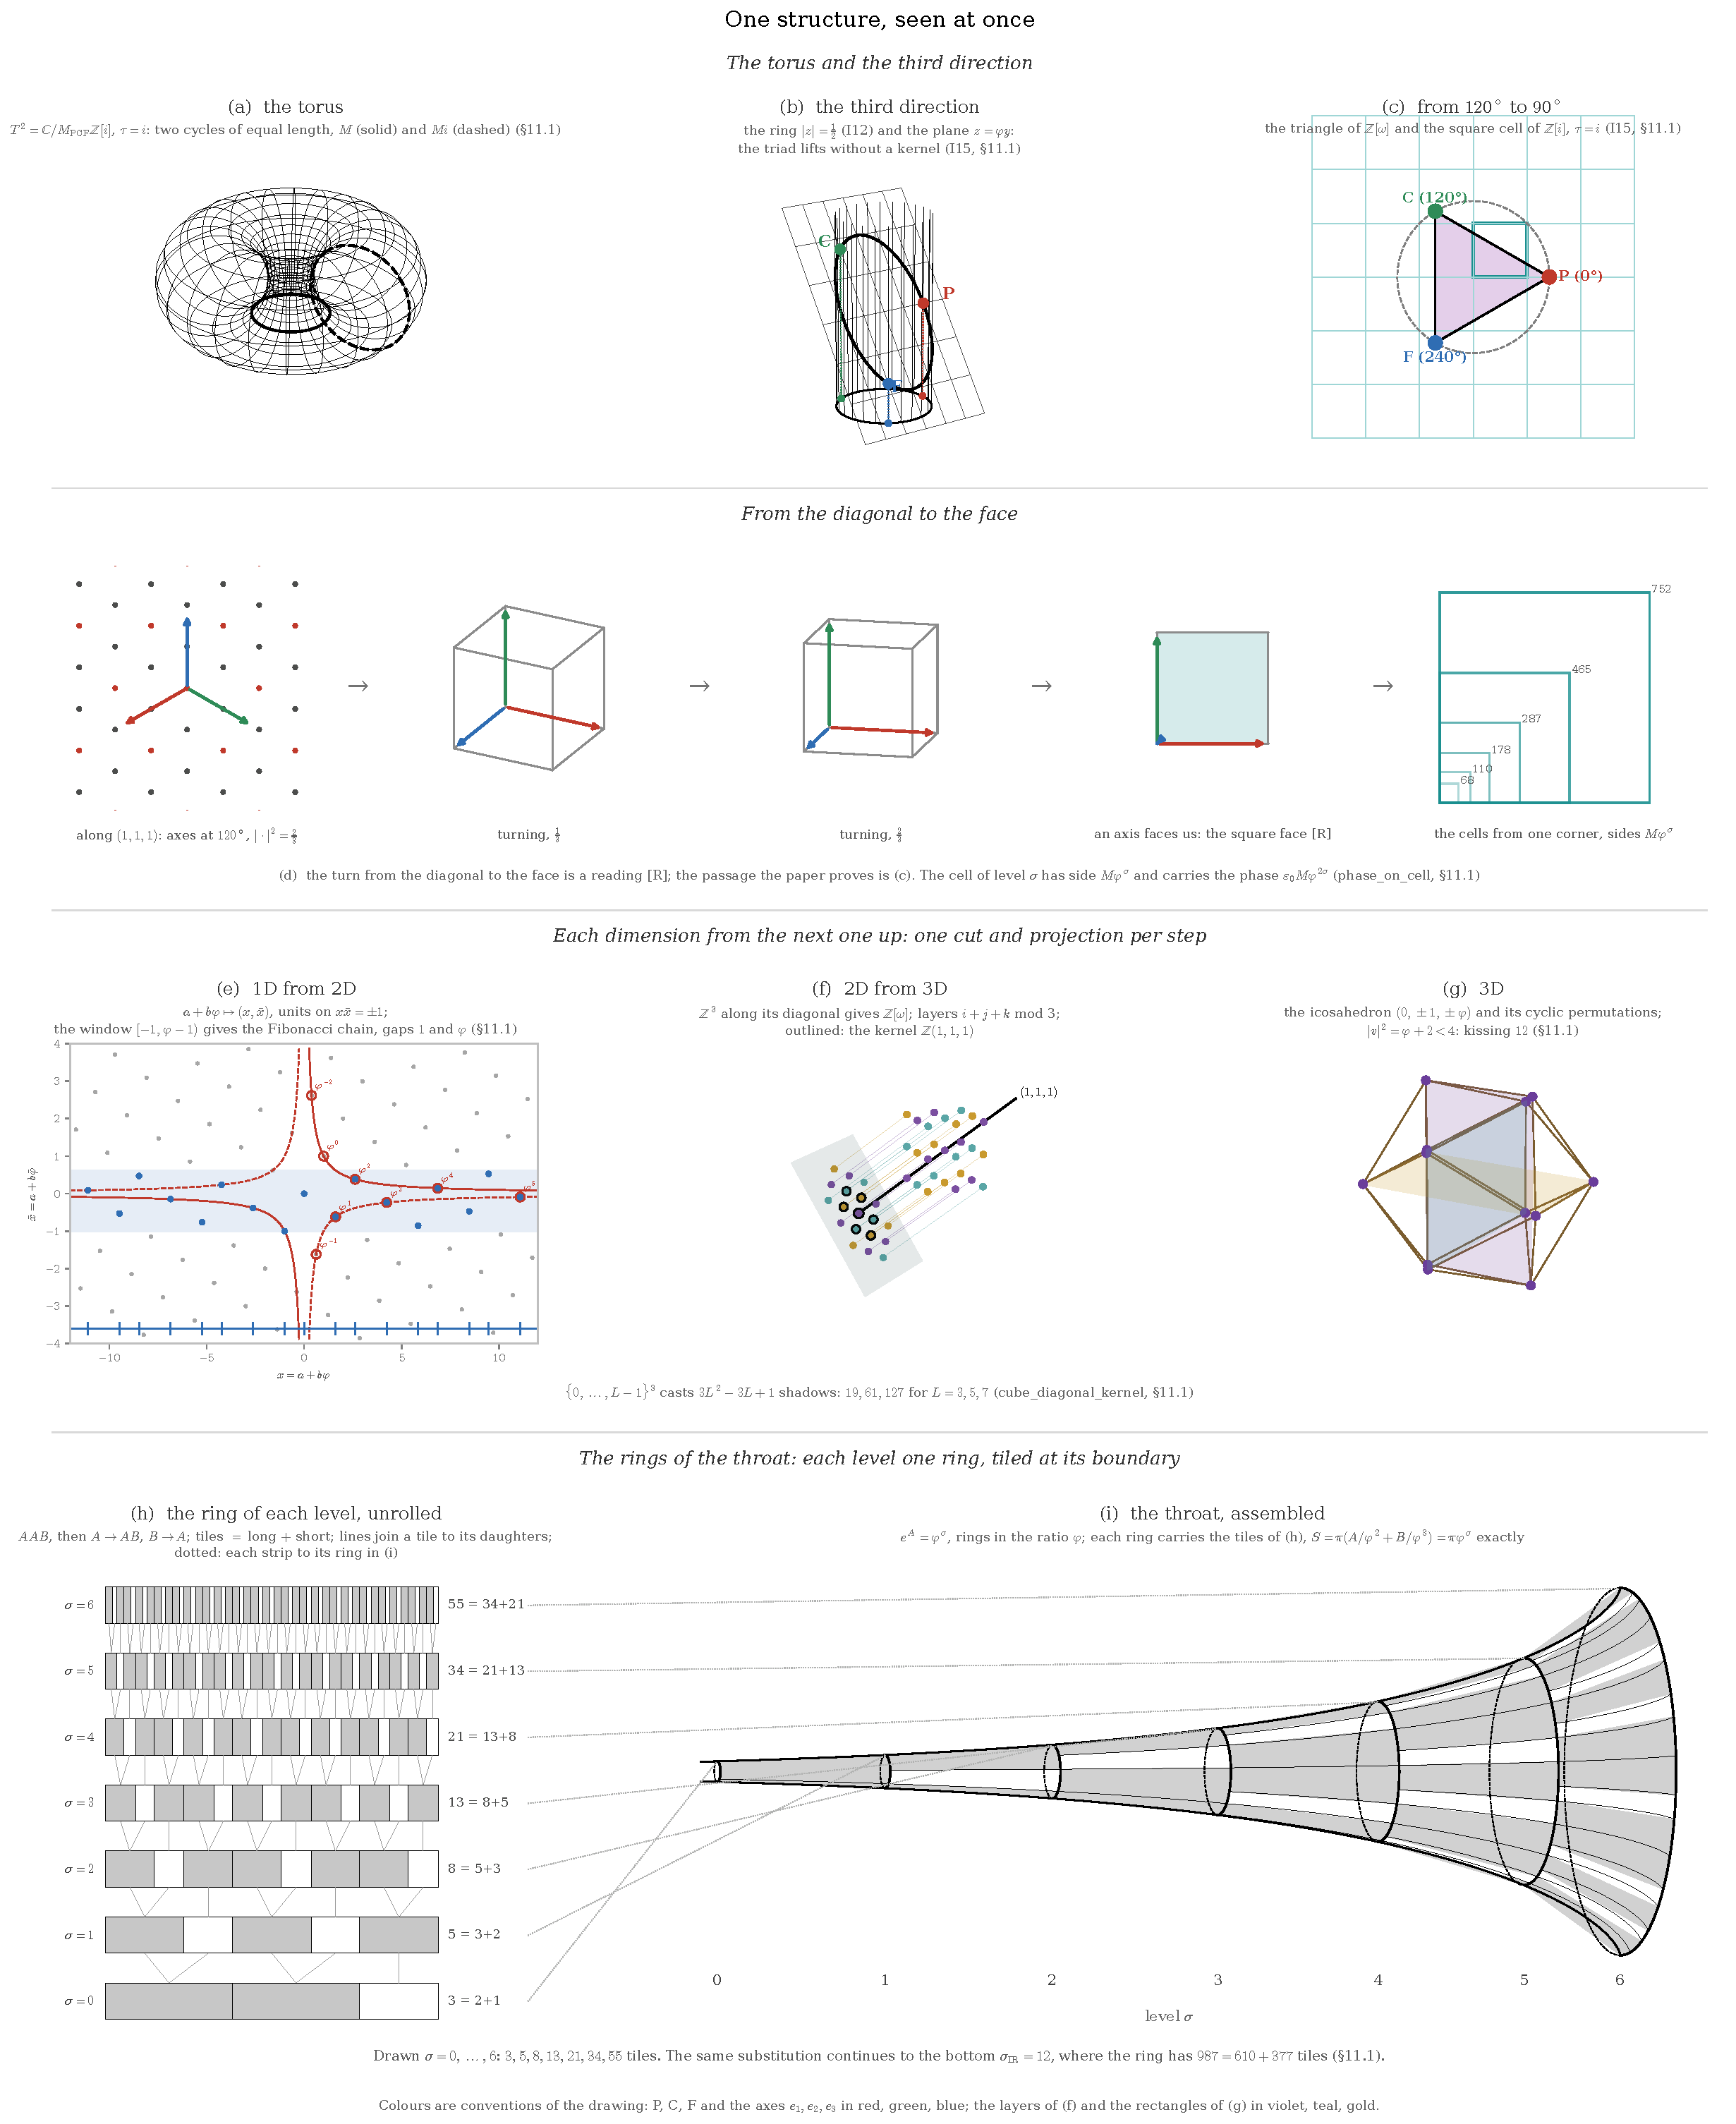
\includegraphics[width=0.85\textwidth]{fig_background.pdf}
\caption{\footnotesize One structure, seen at once. (a)~The torus $T^2=\mathbb C/M_{\mathrm{PCF}}\mathbb Z[i]$, $\tau=i$: two cycles of equal length, $M$ solid and $Mi$ dashed. (b)~The third direction: the ring $|z|=\tfrac12$ and the plane $z=\golden y$: the triad lifts without a kernel. (c)~From $120^\circ$ to $90^\circ$: the triangle of $\mathbb Z[\omega]$ and the square cell of $\mathbb Z[i]$. (d)~From the diagonal to the face: $\mathbb Z^3$ seen along $(1,1,1)$ has its axes at $120^\circ$ with squared length $\tfrac23$; the turn is a reading, and the passage the paper proves is (c); the cell of level $\sigma$ has side $M_{\mathrm{PCF}}\golden^\sigma$ and carries the phase $\varepsilon_0M_{\mathrm{PCF}}\golden^{2\sigma}$ \code{phase\_on\_cell}. (e)--(g)~Each dimension from the next one up: one cut and projection per step. (e)~1D from 2D: $a+b\golden\mapsto(x,\bar x)$, units on $x\bar x=\pm1$; the window $[-1,\golden-1)$ gives the Fibonacci chain, gaps $1$ and $\golden$. (f)~2D from 3D: $\mathbb Z^3$ along its diagonal gives $\mathbb Z[\omega]$; layers $i+j+k$ mod $3$; outlined: the kernel $(1,1,1)$; the cells cast $3L^2-3L+1$ shadows, $19,61,127$ for $L=3,5,7$. (g)~3D: the icosahedron $(0,\pm1,\pm\golden)$ and its cyclic permutations, $|v|^2=\golden+2<4$: kissing $12$. (h)--(i)~The rings of the throat: each level one ring, tiled at its boundary, drawn at $\sigma=0,\dots,6$. (h)~The ring of each level, unrolled: $AAB$, then $A\to AB$, $B\to A$; tiles $=$ long $+$ short; lines join a tile to its daughters, dotted from each strip to its ring in (i). (i)~The throat, assembled: $e^{A}=\golden^{\sigma}$, rings in the ratio $\golden$, each ring carrying the tiles of (h), with $S=\pi(A/\golden^2+B/\golden^3)=\pi\golden^{\sigma}$ exactly, down to $\sigma_{\mathrm{IR}}=12$, where the ring has $987=610+377$ tiles. Colours are conventions of the drawing. Used in \S\ref{ssec:math} and Figure~\ref{fig:throattiling}.}
\label{fig:background}
\end{figure}
It needs no selection of the vacuum that depends on measurement, in the anthropic sense: its values
are derived from the structure, unlike the landscape of string theory and any holographic description
that inherits it, where the parameters of the boundary theory are inputs fixed by data. It is congruent with the axioms of quantum theory and of holography in the sense the introduction states: it carries a mathematical signature of each criterion, not the criterion itself.

It has the signatures of the criteria of Witten and of Chandrasekaran, Longo, Penington and Witten
for an observer in de~Sitter, with the three types of von Neumann algebras in the
tower~\cite{Wit01,CLPW23,Wit24}.

We compare it with the Kaluza--Klein particles, which suggest a fifth dimension~\cite{Kal21,Kle26,LYR26}; here that
dimension appears as a reading of the tower, its throat, and not as a postulate.

\subsection{This article}
In this article we prove the mathematical part of the most recent model and contrast its physical
identifications where the data reach them. We focus on one object, the golden throat, and on what
fixes its spectrum. The argument starts from the data and from what the framework supplies; four
independent conditions then fix the measure, the boundaries, the phase and the bottom, and one fact
fixes the scale; the spectrum so fixed is contrasted with the graviton candidates and with the
cosmological constant; and the two retroductions that close it say what the structure is in
mathematics and what it represents in physics, where the observer is placed: what it is, what it
reaches, and the history of the levels that ends in the observed constant.
Figure~\ref{fig:background} gathers the structure that the proofs use.

\section{The data}\label{sec:data}

The graviton candidates of~\cite{LYR26} are
\begin{equation}\label{eq:data}
  m=(380,\,700,\,1000,\,1322)\ \mathrm{GeV},\qquad
  \frac{m_k}{m_1}=(1,\,1.842,\,2.632,\,3.479).
\end{equation}
The zeros of $J_1$ give $(1,\,1.831,\,2.655,\,3.477)$; with the scale as the only parameter the
residual is $0.54\%$; for predicted ratios $\mu_k$ and data $m_k$ the scale is $\lambda=\sum_k m_k\mu_k/\sum_k\mu_k^2$ and the residual is $\bigl(\tfrac14\sum_k((m_k-\lambda\mu_k)/m_k)^2\bigr)^{1/2}$. The spacing is linear with an offset,
$j_{1,k}\simeq\pi(k+\tfrac14)$. Of the widths quoted in~\cite{LYR26}, only
$\Gamma(700)=20\pm7$~GeV is measured; the others follow the warped-model law
$\Gamma\simeq0.06\,x^{3}$~GeV, with $x=m/(100\ \mathrm{GeV})$. The gluon candidates are a first excitation between $3.6$ and
$4.0$~TeV and a second at $8.6$~TeV. \cite{LYR26} quotes no mass errors for the graviton
candidates; to judge resolution we assume $\pm20$~GeV at $380$ and $700$, $\pm30$ at $1000$ and
$\pm40$ at $1322$. These candidates are identified in~\cite{LYR26} as Kaluza--Klein gravitons
of the two-brane model, so their pattern already carries that reading; the uncertainties are ours,
and every significance quoted below depends on them. The candidates are indications that Le~Yaouanc
and Richard identify in public ATLAS and CMS data, presented by them and not by the collaborations;
they describe some of the effects as marginally significant~\cite{LYR25,LYR26}. Of the four, the
candidates at $380$ and $700$~GeV are reported as evidence; those at $1000$ and $1322$~GeV are the
resonances that, in the two-brane reading, should appear next~\cite{LYR26b}. Where the note compares
ratios it uses the four values as the pattern of~\cite{LYR26}; where it estimates the scale and
contrasts the level it uses the two observed, and the masses it gives at $1028$ and $1346$~GeV are
predictions, to be set against $1014$ and $1328$, the two-brane fit to the same two candidates.

The level of the observer uses the observed cosmological constant,
$\Lambda_{\mathrm{obs}}=3H_0^2\Omega_\Lambda$, with the Planck values~\cite{Pla18}. Its uncertainty is
systematic as well as statistical: the local measurement gives $H_0=73.04\pm1.04$~km\,s$^{-1}$\,Mpc$^{-1}$~\cite{Rie22},
and combinations of DESI data prefer an evolving dark energy at $2.8$ to $4.2$ standard
deviations~\cite{DESI25}, in which case $\Lambda_{\mathrm{obs}}$ is not one number. Within $\Lambda$CDM, the
baryon acoustic oscillations of DESI combined with the cosmic microwave background give
$H_0=68.17\pm0.28$~km\,s$^{-1}$\,Mpc$^{-1}$ and $\Omega_m=0.3027\pm0.0036$, with correlation
$-0.975$~\cite{DESI25}; this is the determination against which the level of the observer is
contrasted.

\section{What the framework supplies}\label{sec:inputs}

The note rests on three kinds of axiom. Each is stated below in full, with what it says and
where it is used, so that the argument can be followed without the Lean file.

\subsubsection*{Mathematical axioms}

These are tools for proving. What they state is true or false by proof, whether or not any
physical system realises it; they make no claim about the world.

\begin{description}
\item[(M1) The theorems of Mathlib.] The note uses standard results of Lean's mathematical library,
in seven groups:
\begin{itemize}
\item \emph{powers and logarithms}: $b^{x+y}=b^xb^y$, $b^{xy}=(b^x)^y$, $b^x>0$ for $b>0$, $\log$ and
$\exp$ inverse, and the strict monotonicity of $x\mapsto b^x$ for $b>1$
(\code{Real.rpow\_add}, \code{Real.rpow\_mul}, \code{Real.rpow\_pos\_of\_pos},
\code{Real.exp\_log}, \code{Real.rpow\_lt\_rpow\_left\_iff});
\item \emph{trigonometry}: $\cos(\pi/5)=(1+\sqrt5)/4$, $\cos(\pi/3)=\tfrac12$,
$\sin(\pi/3)=\sqrt3/2$, $\cos2x=2\cos^2x-1$, $\sin^2x+\cos^2x=1$, $\tan(\arctan x)=x$
(\code{Real.cos\_pi\_div\_five}, \code{Real.cos\_pi\_div\_three}, \code{Real.sin\_pi\_div\_three},
\code{Real.cos\_two\_mul}, \code{Real.sin\_sq\_add\_cos\_sq}, \code{Real.tan\_arctan});
\item \emph{complex numbers}: $i^2=-1$, $e^{i\pi}=-1$, $e^{2\pi i}=1$, $|e^{i\theta}|=1$
(\code{Complex.I\_sq}, \code{Complex.exp\_pi\_mul\_I}, \code{Complex.exp\_two\_pi\_mul\_I},
\code{Complex.abs\_exp\_ofReal\_mul\_I});
\item \emph{numbers and groups}: $\sqrt p$ is irrational for a prime $p$; an integer multiple of an
irrational is irrational and is not an integer; a number whose power is algebraic is algebraic;
$|A_5|=60$ (\code{Nat.Prime.irrational\_sqrt}, \code{Irrational.int\_mul},
\code{IsAlgebraic.of\_pow}, \code{two\_mul\_card\_alternatingGroup});
\item \emph{finite computation}: equalities of $2\times2$ matrices over $\mathbb{Z}$ and over
$\mathbb{Z}/N$, decided by evaluation (the orders of $S$, $ST$ and of the Fibonacci matrix modulo $N$);
\item \emph{modular forms}: the law of the theta series under $S$,
$\vartheta(-1/\tau)=(-i\tau)^{1/2}\vartheta(\tau)$ (\code{jacobiTheta\_S\_smul});
\item \emph{integration}: the Gaussian integral $\int_{\mathbb R}e^{-bx^2}dx=\sqrt{\pi/b}$ for $b>0$
(\code{integral\_gaussian}).
\end{itemize}
\item[(M2) Five classical results that Mathlib does not yet contain.] Each enters Lean as an axiom
with its source, and each is used only where the text says:
\begin{enumerate}
\item \emph{The zeros of $J_1$}~\cite{Wat44}: they increase, the first four are $3.8317$, $7.0156$,
$10.1735$ and $13.3237$, and $j_{1,k}-\pi(k+\tfrac14)\to0$ (McMahon). Used in Theorem~\ref{thm:bessel}
and for the count of modes.
\witness{P}{bessel\_J1\_zeros}
\item \emph{The transcendence of $e^{\pi a}$ for every real algebraic $a\neq0$}, the case $(-1)^{-ia}$ of the Gelfond--Schneider
theorem~\cite{Sch35}. From it the note proves that $e^{\pi}$ is transcendental and $\log\golden/\pi$ irrational, and that the growth $e^{S}$ of the dimension of a level is not a power of an integer (W2).
\witness{P}{exp\_pi\_mul\_algebraic\_transcendental, exp\_pi\_transcendental, level\_growth\_not\_power}
\item \emph{The derivatives of the stereographic meridian}: with $r(b)=\sqrt2-\sin b$,
$(1/r)'=\cos b/r^2$ and $(\cos b/r)'=(1-\sqrt2\sin b)/r^2$, the quotient rule. From them the note
proves that the projection of the square torus is conformal.
\witness{P}{stereographic\_meridian\_deriv}
\item \emph{The law of the Dedekind $\eta$ under $T$}~\cite{Apo90}: $\eta(\tau+1)=e^{2\pi i/24}\eta(\tau)$.
From it the note proves the modular invariance of the string partition function and the phase
$-1$ of $\eta^{12}$.
\witness{P}{dedekindEta, eta\_T}
\item \emph{Weyl's equidistribution}~\cite{Wey16}: for $\alpha$ irrational and $f$ continuous of
period $1$, the averages $\tfrac1N\sum_{n<N}f(n\alpha)$ tend to $\int_0^1f$. From it the note proves factorisation along an
orbit.
\witness{P}{weyl\_equidistribution}
\end{enumerate}
\end{description}

\subsubsection*{Axioms that are mathematical and physical at once}

Each is one statement that the framework reads on both sides throughout. Its mathematical side is
an axiom and is used in proofs. Its physical side is an identification, the most basic of the
framework: it is made everywhere rather than at one place, and it is tested only together with the
axioms (F), through the data.

\begin{description}
\item[(B1) The modulus, $|\Omega|=\tfrac12$.] \emph{Mathematics:} $\tfrac12$ is the fixed point of
$x\mapsto1-x$, and $\golden^{-\log_\golden2}=\tfrac12$. \emph{Physics:} the area quantum $1/(4G_N)=\tfrac12$ per unit area of the
gravitational unit $\ell=\sqrt2\,\ell_P$, the Bekenstein--Hawking $\tfrac14$ per Planck area,
which~\cite{CW6} calls one bit per Planck area and which is a quantum of area, not a Shannon bit,
that would be $\log2$ per area \tier[\testref{test\_shannon\_bit\_against\_the\_area\_law}]{N}; the
spin $\tfrac12$, and the reason the monodromy of the fibre is $\pi$ and not $2\pi$
(Imported statement~\ref{imp:monodromy}). Used in the bottom (Proposition~\ref{prop:twelve}), the
fibre and the crossing point (Corollary~\ref{cor:crossing}).
\item[(B2) The scale, $\golden^2=\golden+1$.] \emph{Mathematics:} the golden ratio, and the additive
law $\golden^{\sigma}+\golden^{\sigma+1}=\golden^{\sigma+2}$ that only $\golden$ satisfies (Imported
statement~\ref{imp:additive}). \emph{Physics:} the step of scale of the tower, its radial direction
$z(\sigma)=\golden^{\sigma}$. Used in the factor $\golden$ (\S\ref{sec:scale}) and throughout.
\item[(B3) The angle, $i^2=-1$.] \emph{Mathematics:} the circle and its roots of unity, and
$\golden=2\cos(\pi/5)$ among them. \emph{Physics:} the angular direction, the standing waves of the
modes, the half-turn and the quarter-turn of their phase. Used in the factor $\pi$
(\S\ref{sec:arity}) and the clock.
\item[(B4) Reflection positivity.] \emph{Mathematics:} $\langle f,e^{-aK}f\rangle\ge0$ for every $f$ and
$a\ge0$, a property an operator has or lacks in a given inner product; \S\ref{sec:operator} proves
which, so on this side it is not an axiom. \emph{Physics:} the Osterwalder--Schrader
axiom that makes a Euclidean theory reconstructible as a physical one~\cite{OS73}. It is imposed, and
it selects the measure $e^{4A}$ (\S\ref{sec:operator}).
\end{description}

\subsubsection*{Physical axioms}

Each identifies a mathematical object with a physical one. These are the claims about the world.
The graviton candidates of \S\ref{sec:data} test (F1)--(F4); the cosmological constant, read with
(F8), tests the lattice form of the observer's level, not (F8) itself; (F5)--(F9) give readings that
the present data do not reach, and (F10) a history that requires $w=-1$, in tension with the
evolving dark energy that the present data prefer.

\begin{description}
\item[(F1) The unit.] The pure number $M_{\mathrm{PCF}}=6\sqrt3\pi/\log\golden=67.846$ is read as the
charged-lepton scale $M=313.84$~MeV, the scale from which
$\sqrt{m_k}=\sqrt M\,\bigl(1+\sqrt2\cos(\tfrac29+\tfrac{2\pi k}{3})\bigr)$ reconstructs the electron,
muon and tau masses to ${\sim}10^{-4}$~\cite{CW6} \tier[\testref{test\_koide\_scale\_and\_unit}]{N}; this is Koide's
relation~\cite{Koi82,Koi83} in Brannen's parametrisation~\cite{RG05}, to which the framework adds the
phase $\delta=2/n^2=\tfrac29$ from the arity and the identification of its scale with
$M_{\mathrm{PCF}}$, which fixes the unit $M/M_{\mathrm{PCF}}=4.626$~MeV; and the scale of the
operator is $m_0=M$. Used in Proposition~\ref{prop:scale} and in every mass.
\item[(F2) The dimension.] The arity $n=3$ of the eigenvalue triangle is mathematics; that $d=n+1=4$
is the dimension of spacetime is physics. Used in Corollary~\ref{cor:phase}.
\item[(F3) Four-dimensional gravity.] The four-dimensional graviton exists as a massless mode of the
throat, which requires Neumann conditions at both ends. Imposed in \S\ref{sec:spectrum}.
\item[(F4) The bottom.] The element $\golden^{12}$, the half-turn of the clock, is the bottom of the
throat, $\sigma_{\mathrm{IR}}=12$. Used in Proposition~\ref{prop:twelve}; tested by
$\sigma_{\mathrm{IR}}=11.97\pm0.05$, from the two observed candidates.
\item[(F5) The Clausius relation.] That the bits, the modes of matter, the horizon entropy and the
entropy of Jacobson's relation are equal as numbers, once each is defined as $\pi\golden^{\sigma}$
in~\cite{CW6}, and that the premises of Jacobson's construction hold on the throat once $G_N$ is read as
$|\Omega|$ (the physical side of (B1)), are mathematics
(Imported statement~\ref{imp:weld} and its proof). That $\delta Q=T\,\delta S$ holds across every
local Rindler horizon of the throat, Jacobson's postulate~\cite{Jac95}, is physics; with it, by
Jacobson's theorem, the four quantities are one mechanism, the one whose equation of state is the
Einstein equation. Used in \S\ref{ssec:phys}.
\item[(F6) The compact circle.] That the circle of each level has the two radii $z(\sigma)$ and
$\tau(\sigma)$ with $z\tau=M_{\mathrm{PCF}}$ is mathematics; that a closed string winds it, with
$\alpha'=M_{\mathrm{PCF}}$, is physics. Since the spectrum of a closed string is the same at radius $R$ and at
$\alpha'/R$, which of the two radii is called the compactification is not part of the claim. Used in
\S\ref{ssec:phys}.
\item[(F7) The level of the boundary.] That the number $N(\sigma)=\golden^{2\sigma}$ of loops on a ring
satisfies $2\pi\sqrt{c\,(N/2)/6}=S(\sigma)$ for $c=3$ is mathematics; that $N/2$ is the level $L_0$ of
the two-dimensional boundary theory of Imported statement~\ref{imp:adscft}, so that $S$ is its Cardy
entropy, is physics. Used in \S\ref{ssec:phys}.
\item[(F8) The cosmological constant of a level.] That the level carries
$\Lambda(\sigma)=6\golden^{-\sigma}=3H_{\mathrm{dS}}(\sigma)^2$ (Imported statement~\ref{imp:weld}), that the throat
has $\Lambda_5=-6$ (its proof, item (d)), and that a rotation $t\mapsto it$ changes the sign of a
square, $(it)^2=-t^2$ \tier[wick\_squares\_flip\_sign]{P}, are mathematics. That $\Lambda(\sigma)$ is
the cosmological constant of the static patch of an observer at level $\sigma$, the anti-de~Sitter
throat being turned into that de~Sitter patch by this internal rotation~\cite{CW6}, is physics. That
the curvature is read in the gravitational unit $\ell=\ell_P/\sqrt{G_N}=\sqrt2\,\ell_P$, the unit to
which $G_N=\tfrac12$ is relative (Imported statement~\ref{imp:adscft}, item (d) of its proof), is the
choice of unit, made by an argument independent of the data. Used in \S\ref{ssec:phys}.
\item[(F9) Where gravity turns on.] That the weight of the window on the unit $\golden^n$ is
$e^{-\pi\golden^{-2n}}$, that its mirror coordinate is $\golden^{-n}=\Lambda(n)/6$, and that the
weight is the first winding term of a heat kernel on the ring (Imported statement~\ref{imp:gauss}),
are mathematics. That the weight measures the curvature of the patch against that of the bulk, and
that four-dimensional gravity turns on where it passes $\tfrac12$, is physics. Used in
\S\ref{ssec:phys}.
\item[(F10) The history of the levels.] That the four-dimensional area law, $4\pi z^2/(4G_N)=2\pi z^2$ with $G_N=\tfrac12$, holds the bits $S=\pi z$ of a level only down to $z=\tfrac12$, $\sigma=-\log_\golden2$, where $S=\pi/2$, half a cell, one doubling below the level $0$, where $S=\pi$ (Imported statement~\ref{imp:valuation}) \tier[area\_law\_4d\_meets\_weld\_iff, capacity\_exceeded]{P} (\testref{test\_the\_compression\_limit\_is\_half\_a\_cell}); and that the first patch has the constant of the throat, $\Lambda(0)=3/G_N=6$ by the entropy law of W4 with $S(0)=\pi$ and $|\Lambda_5|=d(d-1)/2=6$ by W8, which agree only at $d=4$ with $G_N=\tfrac12$ \tier[dS\_entropy\_law, two\_routes\_to\_six]{P}, the level at which they meet being $\sigma=0$ by construction \tier[flip\_level]{P}, are mathematics. That these are the stages of one history, in the unit $\ell$ of (F8), is physics: from the empty space, whose image at the centre of the throat is superpoint-like, the observers accumulate; the anti-de~Sitter throat, with $\Lambda_5=-6$ throughout, compresses what they accumulate towards its centre, each level holding its own bits in a smaller ring, through the level $0$ and down to the limit of compression at $z=\tfrac12$, where the capacity of the four-dimensional area law saturates on half a cell; the saturation causes the burst, the Big Bang, and the burst is the rotation of (F8): what is released is de~Sitter, with the size of the constant of the throat and its sign turned; the radius doubles, half a cell becomes one, and the level $0$, crossed now for the second time, is the first patch of the tower, of the Planck size, $|\Lambda(0)|=|\Lambda_5|$; from there the observers go on accumulating, the level of their horizon rises, and the curvature of the observer's horizon, $3H^2=6\pi/S_H$, falls from $6$ to its asymptotic value $\Lambda_{\mathrm{obs}}$, which is constant. Used in \S\ref{ssec:phys}; contrasted with the equation of state of dark energy, since it requires $w=-1$.
\end{description}
The data are the graviton and gluon candidates of~\cite{LYR26}, read in the two-brane model, with
the uncertainties of \S\ref{sec:data}, and the cosmological constant of \S\ref{sec:data}. They are
not an axiom.

Every theorem of the note rests on (M) and on the mathematical side of (B); every claim about the
world names the physical side of (B), or the (F), that it uses. The usual postulates of quantum field theory, holography and the string are not assumed:
they are imposed, derived or re-derived where they appear.

The construction uses the following statements of
the Crystalline Worldsheet~\cite{CW6} and of the pentagonal $\mathbb{F}_1$-descent~\cite{F1}, which
are theorems there of the axioms (B1)--(B3). They are collected here so that the note can be read on its
own, and this note's Lean module proves several of them again.

\begin{imported}[The tower and its scale operator; \cite{CW6}, eqs.~(81)--(82), Remark~3.7]\label{imp:tower}
The levels $\sigma$ carry the throat coordinate $z(\sigma)=\golden^{\sigma}$ and the self-adjoint scale
operator $H|\sigma\rangle=m_0\golden^{\sigma}$, with $m_0$ left free. The framework supplies two spectra
from the pair $\pi,\golden$ and keeps them apart: the golden tower is the radial and scale tower, read as the scale of the Kaluza--Klein spectrum on the gravity side; the confining spectrum is the Regge tower
$\alpha'M_n^2=n$ on the gauge side.
\witness{P}{in~\cite{CW6}}
\end{imported}

\begin{imported}[The Kaluza--Klein operator; \cite{CW6}, Appendix~A.1, eqs.~(158)--(159)]\label{imp:A1}
On the $2n+1$ levels $\sigma=0,\dots,2n$ the Kaluza--Klein operator is the second difference with
golden hoppings $\golden^{2}$ and $\golden^{-2}$ and step $\log\golden$; its eigenvalues are
$m_k^2=4\sin^2\bigl(k\pi/(4(n+1))\bigr)/(\log\golden)^2$, $k=1,\dots,2n+1$, all positive (eq.~(160)
there). The continuous interior mode has $m^2_{\mathrm{KK}}\approx-4.318$, below the
Breitenlohner--Freedman bound $m^2_{\mathrm{BF}}=-d^2/4=-4$. \tier{P} in~\cite{CW6}; the comparison
with the bound.
\witness{P}{log\_golden\_lt\_half}
\end{imported}
\noindent The golden numbers are the levels of this operator, $z(\sigma)=\golden^{\sigma}$, not its eigenvalues: for $n=6$ the ratios of successive masses are $1.99,1.48,\dots,1.02$. What Imported statement~\ref{imp:tower} reads as golden is the scale at which each level sits \tier[\testref{test\_mass\_ratios\_of\_imp\_a1}]{N}.

\begin{imported}[The arity; \cite{CW6}, \S2.2 and Appendix~A.7]\label{imp:arity}
The golden central chain $\golden^2+\golden^{-2}=3$ fixes the arity $n=3$, and $d=n+1=4$.
\witness{P}{sq\_add\_inv\_sq}
\end{imported}

\begin{imported}[The scale; \cite{CW6}, eq.~(31), Theorems~5.33 and~5.35; \cite{F1}; \cite{HP26}, the certainty principle]\label{imp:scale}
$\varepsilon_0=\log\golden/(6\sqrt3)$ and $M_{\mathrm{PCF}}=6\sqrt3\,\pi/\log\golden$, so that
$\varepsilon_0M_{\mathrm{PCF}}=\pi$, and $\log\golden=6\sqrt3\,\pi/M_{\mathrm{PCF}}$: the scale is
where $\pi$ and $\log\golden$ meet. The half-turn $\pi$ that fixes it is $2\pi\mu$, with
$\mu=\tfrac12$ the common modulus of the microstate. $M_{\mathrm{PCF}}=67.846$ is a pure number; the
identification $M=M_{\mathrm{PCF}}$ of~\cite{CW6} (\code{M\_eq\_Mpcf} there) with the
charged-lepton scale $M=313.84$~MeV fixes the unit of the framework, $M/M_{\mathrm{PCF}}=4.626$~MeV, and
every relation of $M$ with $\pi$ and $\log\golden$ below is written in that unit; its placement face, the proton five steps of action $\pi$ above the
electron, gives $m_p/3=312.8$~MeV.
\witness{P}{certainty\_principle, log\_from\_scale}
\end{imported}

\begin{imported}[The monodromy; \cite{CW6}, Proposition~2.24 and Remark~4.11]\label{imp:monodromy}
The monodromy of the fibre is the half-turn $e^{i\pi}=-1$, $\pi$ and not $2\pi$, because
$\mu=\tfrac12$; the clock of the accumulation, the ultraviolet fixed point and the certainty
principle $\varepsilon_0M_{\mathrm{PCF}}=\pi$ are one $\golden$-fact. The same modulus
$\tfrac12$, the self-conjugate midpoint of $x\mapsto1-x$, is the fermion spin (\cite{CW6},
Proposition ``Fermion and Standard-Model content''). \tier{P} in~\cite{CW6};
the half-turn and its order.
\witness{P}{fibre\_half\_turn}
\end{imported}

\begin{imported}[The two lengths; \cite{CW6}, eq.~(111); \cite{F1}, the two lengths of the tower]\label{imp:lengths}
The throat coordinate $z(\sigma)=\golden^{\sigma}$ and the weld time
$\tau(\sigma)=M_{\mathrm{PCF}}\golden^{-\sigma}$ satisfy $z(\sigma)\tau(\sigma)=M_{\mathrm{PCF}}$ at every
level. This is $R\cdot(\alpha'/R)=\alpha'$ with $\alpha'=M_{\mathrm{PCF}}$: short and long distance are
one family exchanged by T-duality.
\witness{P}{lattice\_radius\_conjugate}
\end{imported}

\begin{imported}[The additive law of the tower; \cite{F1}]\label{imp:additive}
$\golden^{\sigma}+\golden^{\sigma+1}=\golden^{\sigma+2}$ for every real $\sigma$; conversely, a positive
$r$ with $r^{\sigma}+r^{\sigma+1}=r^{\sigma+2}$ for some real $\sigma$ satisfies $r^2=r+1$, whose only
positive root is $\golden$.
\witness{P}{additive\_law\_forces\_golden}
\end{imported}

\begin{imported}[The golden valuation; \cite{F1}, the golden valuation and the $2$-adic anchor]\label{imp:valuation}
With $v(x)=\log x/\log\golden$, $v(\golden^{n})=n$, and $x>0$ lies on the tower exactly when $v(x)$ is
an integer. With $\lambda=\log2/\log\golden$, $|2|_2=\tfrac12=\golden^{-\lambda}$: a power of $2$ and a
level of $\golden$ are one quantity, in the unit $\lambda$.
\witness{P}{golden\_valuation\_on\_tower, two\_adic\_is\_level}
\end{imported}

\begin{imported}[The polar form of $\golden$; \cite{F1}, the polar form and the cyclotomic clock]\label{imp:polar}
At each prime $p\neq5$, $\golden=[\bar\golden]\cdot\langle\golden\rangle$: an angular part, a root of
unity whose order is the order of $\golden$ modulo $p$, times a principal unit, its radial part.
Over $\mathbb{Q}$ the angular origin is already visible: $\golden=2\cos(\pi/5)=\zeta_{10}+\zeta_{10}^{-1}$,
with $\zeta_{10}=e^{i\pi/5}$ a root of the cyclotomic polynomial $\Phi_{10}$, so $\golden$ is a
point of the circle read on its diameter; and $\golden=1+1/\golden$, the relation that makes its
continued fraction $[1;1,1,\dots]$.
\witness{P}{golden\_eq\_two\_cos\_pi\_div\_five,
golden\_self\_reference}
\end{imported}

\begin{imported}[The clocks; \cite{Wall60,Ser73,Ser71}]\label{imp:clocks}
The order of $\golden$ in $(\mathbb{Z}[\golden]/N)^\times$ is $24$ for $N=16$, $9$, $12$, $24$, $48$ and
$72$, $20$ for $N=5$ and $60$ for $N=10$. In $\mathrm{SL}_2(\mathbb{Z})$, $S$ has order $4$ and $ST$ order $6$,
$ST\equiv\left(\begin{smallmatrix}0&1\\1&1\end{smallmatrix}\right)\pmod2$, $S^2=(ST)^3=-1$, and
$\chi(\mathrm{SL}_2(\mathbb{Z}))=\tfrac14+\tfrac16-\tfrac12=\zeta(-1)$. The orders are Pisano
periods~\cite{Wall60}, computed here; $S=\left(\begin{smallmatrix}0&-1\\1&0\end{smallmatrix}\right)$
and $T=\left(\begin{smallmatrix}1&1\\0&1\end{smallmatrix}\right)$ generate
$\mathrm{SL}_2(\mathbb{Z})$~\cite{Ser73}, and the Euler characteristic is classical~\cite{Ser71}.
The orders modulo $16$, $9$, $5$ and $10$, and those of $S$ and $ST$, are computed in Lean.
\witness{P}{pisano\_orders, modular\_orders}
\end{imported}

\begin{imported}[One exponent, angle and radius]\label{imp:angle}
With $q=e^{2\pi i\tau}$ and $\tau=x+iy$, $q^{E}=e^{2\pi iEx}\,e^{-2\pi Ey}$: a factor of modulus one
and a positive real.
\witness{P}{exponent\_angle\_radius, angle\_has\_modulus\_one}
On the tower the angle and the radius are one quantity: the spectral angle of the level $\sigma$,
$\alpha(\sigma)=\arctan(\varepsilon_0\golden^{\sigma})$, has $\tan\alpha(\sigma+1)/\tan\alpha(\sigma)=\golden$
(\cite{CW6}, Proposition~3.4, eq.~(76)): one step in angle is one step $\golden$ in scale.
\witness{P}{spectral\_angle\_ratio}
\end{imported}

\begin{imported}[One microstate at every level; \cite{CW6}, \S3.4]\label{imp:adscft}
The single microstate $\Omega$, with $|\Omega|_\sigma=\tfrac12$ at every level $\sigma$, gives at each
level the isometric bulk--boundary map $V^{\dagger}V=\mathbf 1$, the area law
$S_{\mathrm{BH}}=1/(4G_N)=\tfrac12$ and the Brown--Henneaux central charge $c=3$, whence the GKPW
dictionary and the Ryu--Takayanagi formula: the correspondence holds from one microstate, not from
an ensemble.
\witness{P}{in~\cite{CW6}}
\end{imported}
\noindent\emph{The mathematical content, proved here.} Write $\Omega(\theta)=\tfrac12e^{i\theta}$ and
$\omega=e^{2\pi i/3}$. Then:
(a) $|\Omega(\theta)|=\tfrac12$ for every $\theta$, so the state is the same single state at every
level \tier[worldline\_modulus]{P};
(b) the eigenvalue triad $v_k=\tfrac12\omega^{k}$, $k=0,1,2$, has $|v_k|=\tfrac12$
\tier[triad\_modulus]{P}, hence $\|v\|^2=3\cdot\tfrac14=\tfrac34$, and the normalised column
$V_k=v_k/\|v\|$ has $V^{\dagger}V=\sum_k|V_k|^2=3\cdot\tfrac{1/4}{3/4}=1$: the map
$z\mapsto(V_0,V_1,V_2)z$ is an isometry \tier[bulk\_boundary\_isometry]{P};
(c) the binary entropy at the modulus is $H(\tfrac12)=-2\cdot\tfrac12\log_2\tfrac12=1$, one bit
\tier[bin\_entropy\_half]{P};
(d) with $G_N=|\Omega|=\tfrac12$, $1/(4G_N)=\tfrac12$ \tier[area\_quantum\_half]{P}, and the
expression $3\ell/(2G)$ with $\ell=1$ equals $3$ if and only if $G=\tfrac12$
\tier[brown\_henneaux\_three\_iff]{P}. Both are relative to the curvature radius $\ell=1$, not to the
unit of (F1); $c=3$ is the quantum regime of the boundary theory, and Cardy's expression applies at
large level;
(e) a single state assigns one number to each source, so the joint value of two sources is the
product of their values, $Z(J_1)Z(J_2)$, with no connected term; a connected term
$\langle Z(J_1)Z(J_2)\rangle-\langle Z(J_1)\rangle\langle Z(J_2)\rangle$ appears only when values are
averaged over several states \tier[single\_theory\_factorizes]{P}.
That $V$ is the bulk--boundary map, $G_N$ the Newton constant, $1/(4G_N)$ the area quantum and $c$
the Brown--Henneaux charge~\cite{BH86} is the physical side of axiom~(B1). The dictionary that turns
these into the correspondence, GKPW~\cite{Mal98,GKP98,Wit98} and Ryu--Takayanagi~\cite{RT06},
enters cited, as in~\cite{CW6}. What the statement adds to the dictionary is that its input is one
state and not an ensemble; that is (a), and with (e) the single theory factorises. In the language of quantum error correction, in which the bulk--boundary map of the correspondence is the encoding of a code~\cite{ADH15,PYHP15}, $V$ is an encoding and $P=VV^\dagger$ the projection onto its code subspace; here that subspace has dimension one, a state and not a space of logical states, which is (a) and (e) said again: one microstate, and no ensemble.

\begin{imported}[Envelope and fluctuations; \cite{F1}, the individual and the ensemble; \cite{CW6}, Remark ``Envelope yes, fluctuations no'']\label{imp:envelope}
A deterministic operator built from $\golden$, without reference to the spectrum it describes,
determines the envelope of that spectrum. The pair-correlation statistics of an ensemble are a
statement about the fluctuations around the envelope.
\witness{P}{in~\cite{F1}}
\end{imported}

\begin{imported}[The weld; \cite{CW6}, \S4.4]\label{imp:weld}
The saturation entropy of the level $\sigma$ is $S(\sigma)=\pi\golden^{\sigma}$, and one number is at once
the bits accumulated by the observer, the modes of matter $\lfloor S(\sigma)\rfloor$, the horizon
entropy $S_{\mathrm{BH}}=A/4G_N$ and the entropy of Jacobson's relation $\delta Q=T\delta S$, from
which the Einstein equation follows. The energy per bit is the same at every level, so that
$S(\sigma)=M_{\mathrm{PCF}}\,\varepsilon(\sigma)$.
\witness{P}{in~\cite{CW6}}
The colour gap of the level is $\Delta_{\mathrm{colour}}=\sqrt{\sigma_{\mathrm{tension}}}>0$, the
root of a string tension $\sigma_{\mathrm{tension}}=q_m^2V$ obtained by monopole condensation, with
$V(\sigma)=\varepsilon_0\golden^{-\sigma}$ and Dirac quantisation $q\,q_m=2\pi$ (\cite{CW6},
Propositions ``Magnetic condensate and the colour gap'' and ``The tension is welded to the tower'')
\tier{P} in~\cite{CW6}; the Hubble rate of the static patch descends the tower in the same way,
$H_{\mathrm{dS}}(\sigma)=\sqrt2\,\golden^{-\sigma/2}$, written with a subscript to keep it apart from the
scale operator $H$ of Imported statement~\ref{imp:tower}, and the cosmological constant of the level is
$\Lambda=6\golden^{-\sigma}$ (\cite{CW6}, Theorem ``The modular generator is the Landau--Lifshitz
boundary charge'' and \S4.3).
The weld is the one point where the three von Neumann types of~\cite{CLPW23} meet: type~I in the discrete count
of modes, type~II in the bits the observer accumulates, type~III in the horizon entropy of
spacetime~\cite[\S4.4]{CW6}.
\end{imported}
\noindent\emph{The premises of Jacobson's construction, proved here.} Jacobson~\cite{Jac95} derives
the Einstein equation from $\delta Q=T\,\delta S$ on every local Rindler horizon, given an entropy
proportional to area with one universal coefficient and the same law at every point. On the throat
these premises are theorems:
(a) the coefficient is universal: $\eta=1/(4G_N)$ with $G_N=|\Omega_\sigma|=\tfrac12$ at every level,
so $\eta=\tfrac12$ everywhere \tier[area\_coefficient\_every\_level]{P};
(b) the law is the same at every level: with $\varepsilon(\sigma)=\varepsilon_0\golden^{\sigma}$ and
$\varepsilon_0M_{\mathrm{PCF}}=\pi$, the energy per bit is
$\varepsilon(\sigma)/S(\sigma)=\varepsilon_0/\pi=1/M_{\mathrm{PCF}}$ at every level, a temperature that
does not depend on $\sigma$ \tier[energy\_per\_bit\_constant]{P}; and $\varepsilon(\sigma)\tau(\sigma)=\pi$ \tier[closure\_each\_level]{P} is the shortest time in which a state of two levels with gap $\varepsilon(\sigma)$ becomes orthogonal to itself, the bound of Mandelstam and Tamm and of Margolus and Levitin~\cite{MT45,ML98}: at the half-turn the overlap with its start of a state with weights $1-p$ and $p$ on the two levels is $1-2p$, zero only for $p=\tfrac12$ \tier[orthogonal\_at\_half\_turn]{P}, so each level reaches a distinguishable state in exactly its own time, and only with the weight $\tfrac12$;
(c) each mode carries exactly one bit, a unit of Fisher information: the Fisher information per
eigenvalue is $4\mu^2$, and $4\mu^2=1$ if and only if $\mu=\tfrac12$ \tier[fisher\_unit\_iff]{P}, which
is why the count of modes and the count of bits are one number and not merely close; the bit of this
item is a unit of Fisher information, not of Shannon entropy, and $S(\sigma)$ is an entropy in
natural units: the exact count of states at level $N/2$ grows as $e^{S}$, with slope $1.001$ in $S$,
while $\lfloor S\rfloor$ Shannon bits would carry only a fraction $\log2=0.693$ of it \tier[\testref{test\_entropy\_modes\_and\_bits}, \testref{test\_cardy\_slope\_of\_the\_count}]{N};
(d) the throat is an Einstein space: for $ds^2=e^{2A}\eta_{\mu\nu}dx^\mu dx^\nu+dy^2$ in five
dimensions the Ricci tensor has $R_{\mu\nu}=-(A''+4A'^2)g_{\mu\nu}$ and $R_{yy}=-4(A''+A'^2)$; with
$e^{A}=\golden^{\sigma}$, $y=\sigma\log\golden$, one has $A'=1$, $A''=0$, so $R_{AB}=-4g_{AB}$,
$R=-20$ and $G_{AB}=6g_{AB}$, $\Lambda_5=-6$ \tier[throat\_einstein\_space]{P}; hence
$R_{ab}k^ak^b=0$ for every null $k$, and in vacuum the Clausius relation gives $\delta S=0$, the
equilibrium Jacobson's argument starts from \tier[einstein\_null\_contraction]{P};
(e) the tension is fixed by the entropy level by level:
$(q_m^2\varepsilon_0\golden^{-\sigma})(\pi\golden^{\sigma})=q_m^2\varepsilon_0\pi=4\pi^4/(q^2M_{\mathrm{PCF}})$ at
every level \tier[tension\_times\_entropy\_const]{P}, so $\sigma_{\mathrm{tension}}\propto\golden^{-\sigma}$ and
$\Delta_{\mathrm{colour}}\propto\golden^{-\sigma/2}$, the scaling used below.
What remains is the relation $\delta Q=T\,\delta S$ itself, which is axiom~(F5); given it, the
Einstein equation with $G_N=\tfrac12$ follows by Jacobson's theorem, and the four quantities of the
weld are one mechanism rather than four equal numbers.

\begin{imported}[The golden coupling; \cite{CW6}, Proposition ``The golden coupling: which map is an isometry''; \cite{HP26}, the lattice symmetry bridge]\label{imp:coupling}
The eigenvalue triangle $\tfrac12\omega^{k}$, $\omega=e^{2\pi i/3}$, lies on the hexagonal lattice
$\mathbb{Z}[\omega]$; the golden coupling $z=\golden y$, a third direction tied to the plane by
$\golden$, carries it onto the square lattice $\mathbb{Z}[i]$. The passage from $120^{\circ}$ to $90^{\circ}$
is a change of the group that acts, and $\tau=i$ is the fixed point of the one that survives, the
quarter-turn $S$.
\witness{P}{in~\cite{CW6}}
\end{imported}

\begin{imported}[The tower is the unit group; \cite{F1}, Theorem ``The tower is the unit group, without Dirichlet'']\label{imp:units}
The ring of integers of $\mathbb{Q}(\sqrt5)$ is $\mathbb{Z}[\golden]$, there is no unit in the interval
$(1,\golden)$, and consequently every unit $u>0$ is $\golden^{k}$ for some $k\in\mathbb{Z}$.
classically, Dirichlet's unit theorem~\cite{Neu99}.
\witness{P}{in~\cite{F1}}
\end{imported}
\noindent\emph{The proof, and the lattice it describes.} Write $a+b\golden$ as the pair $(a,b)$;
with $\golden^2=\golden+1$ the product is $(a,b)(c,d)=(ac+bd,\,ad+bc+bd)$ and the norm
$N(a+b\golden)=(a+b\golden)(a+b\bar\golden)=a^2+ab-b^2$ is multiplicative \tier[znorm\_mul]{P}. Since
$N(\golden)=-1$, $N(\golden^n)=(-1)^n$ \tier[znorm\_zpow]{P}: every integer level is a unit, and
$\golden^{12}=89+144\golden$ has norm $1$ \tier[bottom\_is\_lattice\_point]{P}. Conversely, let $u\in(1,\golden)$ be
a unit, with trace $t=u+\bar u\in\mathbb Z$. If $N(u)=1$ then $\bar u=1/u$ and $t=u+1/u\in(2,3)$; if
$N(u)=-1$ then $\bar u=-1/u$ and $t=u-1/u\in(0,1)$; neither interval contains an integer
\tier[no\_unit\_below\_golden]{P}. For any unit $u>0$, with $k=\lfloor\log u/\log\golden\rfloor$, the unit
$u\golden^{-k}$ lies in $[1,\golden)$ and is therefore $1$~\cite{F1}. The map $x\mapsto(x,\bar x)$
carries $\mathbb Z[\golden]$ onto a discrete lattice of the plane, of covolume $\sqrt5$; its units lie
on the hyperbolas $xy=\pm1$, at the points $(\golden^n,\bar\golden^{\,n})$, and since
$\bar\golden=-1/\golden$ \tier[conjugate\_is\_mirror]{P} the second coordinate of a level is its mirror,
$\bar\golden^{\,n}=(-1)^n\golden^{-n}$. A real level $\sigma$ runs continuously along the hyperbola,
$(\golden^{\sigma},\pm\golden^{-\sigma})$, and is a lattice point exactly when $\sigma$ is an integer.
The Galois conjugation exchanges the two coordinates. Multiplied by $M_{\mathrm{PCF}}$, the second coordinate of a level is the weld time of Imported statement~\ref{imp:lengths}: $M_{\mathrm{PCF}}\,|\bar\golden^{\,\sigma}|=M_{\mathrm{PCF}}\golden^{-\sigma}=\tau(\sigma)$, so that $z(\sigma)\tau(\sigma)=M_{\mathrm{PCF}}\,|N(\golden^{\sigma})|=M_{\mathrm{PCF}}$ \tier[weld\_time\_is\_conjugate]{P}. The two lengths that T-duality exchanges are the two coordinates that the Galois conjugation exchanges, and their product is constant because the norm of a unit is $\pm1$; at the bottom, $\tau(12)=0.2107$ (\testref{test\_weld\_time\_at\_the\_bottom}).

\begin{imported}[The self-dual Gaussian; \cite{CW6}, Proposition ``Uniqueness of the self-dual Gaussian'' and Theorem ``Half-factorial'']\label{imp:gauss}
For $g_a(x)=e^{-ax^2}$, $a>0$, with $\widehat g(\xi)=\int g(x)e^{-2\pi ix\xi}dx=\sqrt{\pi/a}\,e^{-\pi^2\xi^2/a}$,
three independent conditions fix $a=\pi$: normalisation $\int g_a=1$, the amplitude of
$\widehat{g_a}$, and its width. The self-dual Gaussian is $g(x)=e^{-\pi x^2}$, $\widehat g=g$,
$\int g=1$; and $\Gamma(\tfrac12)=\sqrt\pi$, $\Gamma(\tfrac32)=\mu\sqrt\pi$ with $\mu=\tfrac12$.
\witness{P}{in~\cite{CW6}}
\end{imported}
\noindent\emph{Proved here.} $\int_{\mathbb R}e^{-ax^2}dx=\sqrt{\pi/a}$, and $\sqrt{\pi/a}=1$ if and
only if $a=\pi$ \tier[gauss\_normalised\_iff, gaussian\_integral\_one\_iff]{P}; this is also the amplitude
condition. The width condition $\pi^2/a=a$ reads $(a-\pi)(a+\pi)=0$, so $a=\pi$
\tier[fourier\_width\_iff]{P}. The $\sqrt\pi$ comes from the circle: the square of the integral is
$\int_{\mathbb R^2}e^{-|x|^2}d^2x=2\pi\int_0^\infty e^{-\rho^2}\rho\,d\rho=\pi$. The same Gaussian is
the Euclidean weight of the free path integral, the factor $e^{iS}$ becoming $e^{-S}$ under the
rotation $t\mapsto it$ of axiom~(F8), and, summed over a lattice, it is the theta series whose law
under $S$ is fixed at $\tau=i$ (M1); the width $\pi$, the point $\tau=i$ and the modulus $\tfrac12$
are fixed points of involutions~\cite[Remark ``One principle, five fixed points'']{CW6}.
Placed on the second coordinate of the lattice of Imported statement~\ref{imp:units}, the Gaussian is
a nome: with $\tau_n=i\golden^{-2n}$ and $q=e^{i\pi\tau}$, the weight of the unit $\golden^n$ is
$e^{-\pi\golden^{-2n}}=q(\tau_n)$, so the levels are a tower of tori of modulus $\tau_n=i/N(n)$,
$N(n)=\golden^{2n}$, that degenerate towards the cusp as $n$ grows. The modular map $S$,
$\tau\mapsto-1/\tau$, the quarter-turn, carries $\tau_n$ to $\tau_{-n}$ \tier[S\_acts\_as\_mirror]{P}: on this
tower it is the Galois mirror. By Poisson summation, the law of the theta series under $S$ (M1),
$\sum_ke^{-\pi k^2N}=N^{-1/2}\sum_me^{-\pi m^2/N}$, so the weight $e^{-\pi/N}$ is the first winding term of
the heat kernel on the ring whose modes are the left side \tier[theta\_S\_law]{P}. At $\tau=i$, the
level $0$, $\vartheta_3(e^{-\pi})=\pi^{1/4}/\Gamma(\tfrac34)$, the lemniscatic value~\cite{WW27}
\witness{N}{\testref{test\_theta3\_at\_tau\_i}}

\subsubsection*{The criteria a single object must meet}

The problem of the note is stated by criteria from three sources, which are kept apart: Witten
(W01)~\cite{Wit01}, Chandrasekaran, Longo, Penington and Witten (CLPW)~\cite{CLPW23}, and
Gibbons--Hawking (GH)~\cite{GH77}. The yardstick is the classification of von Neumann algebras used
by CLPW: type~I, discrete, with minimal projections; type~II, of observation, with a trace; type~III,
of the local field, with neither. What is proved below is the signature of each, not the technical
classification, which is cited. The object is the eigenvalue triangle $\lambda_k=\tfrac12\omega^k$,
$\omega=e^{2\pi i/3}$, with the component norms $\|C\|=1$, $\|F\|=\tfrac{\sqrt3}2$,
$\|P\|=\tfrac1{\sqrt3}$ of~\cite{CW6}, whose product is the modulus $\tfrac12$: $C$ the real
eigenvalue normalised by the circumradius, $F$ the chord between adjacent eigenvalues, and $P$ the
ratio of the apothem $\tfrac14$ to the half-side $\tfrac{\sqrt3}4$.
The twelve premises that follow are labelled W1 to W12.
\begin{description}
\item[\wtag{W1}{CLPW}.] The observer is described by the theory: the projection that places it is internal,
with no region outside. Mathematics: the bulk--boundary map is an isometry, $V^\dagger V=\mathbf 1$
(item (b) of the proof after Imported statement~\ref{imp:adscft}) \tier[bulk\_boundary\_isometry]{P};
then $P=VV^\dagger$ is a projection, $P^2=V(V^\dagger V)V^\dagger=P$ \tier[projection\_of\_isometry]{P},
and it splits the identity, $P+(\mathbf 1-P)=\mathbf 1$ and $P(\mathbf 1-P)=0$
\tier[idempotent\_splits\_identity]{P}: the projection that places the observer is built from the
theory's own map, and nothing is left outside the two. The observer so placed is objective: the
Fisher information per eigenvalue is $4\mu^2$, one bit if and only if $\mu=\tfrac12$
\tier[fisher\_unit\_iff]{P}, and $\tfrac12$ is the threshold at which redundant records make a level
objective~\cite{Kie26,CW6}. Physics: axiom~(F8).
\item[\wtag{W2}{W01}.] The Hilbert space of a level is finite. Its dimension is the number of states of the boundary theory of Imported statement~\ref{imp:adscft}, of central charge $c=3$, at or below the level $L_0=N/2$; it is an integer because the levels $L_0$ of that theory are integers while $N/2=\golden^{2\sigma}/2$ is real, and it is $1654$, $3.4\times10^{6}$ and $8.2\times10^{11}$ at $\sigma=3,4,5$. Its logarithm is $S(\sigma)$ to leading order, by Cardy's formula~\cite{Car86}, with a correction of order $\ln N$: fitted over $\sigma=3,\dots,9$, the slope in $S$ is $0.997$ \tier[\testref{test\_cardy\_slope\_of\_the\_count}]{N}. The count at the level itself, used for the weld (Imported statement~\ref{imp:weld}, item (c) of its proof), grows in the same way, with slope $1.001$. So $e^{S}$, which is not an integer, is the growth of an integer dimension, as the area of a disk is the growth of the integer count of the lattice points inside it~\cite{Hux03}. The level also carries the integer number $\lfloor S(\sigma)\rfloor\ge0$ of modes \tier[witten\_finite\_rank]{P}; \cite{CW6} writes that count as $\dim\mathcal H(\sigma)$, and it is read here as the number of modes.
\item[\wtag{W3}{W01}.] The pairing is positive: the modulus exceeds the collapse threshold of~\cite{CW6},
$\tfrac12>\tfrac14$ \tier[half\_gt\_quarter]{P}; its Osterwalder--Schrader form is the reflection
positivity of the tower.
\item[\wtag{W4}{W01}.] The entropy counts the states, $S=\ln\dim\mathcal H$ to leading order (W2), in natural units, as are the entropies of
Gibbons--Hawking (W9) and of Cardy; the level carries $\lfloor S(\sigma)\rfloor$ modes, and $\Lambda(\sigma)S(\sigma)=6\golden^{-\sigma}\cdot\pi\golden^{\sigma}=6\pi=3\pi/G_N$
with $G_N=\tfrac12$, the entropy law of a de~Sitter horizon \tier[lambda\_times\_entropy, dS\_entropy\_law]{P}.
\item[\wtag{W5}{W01}.] The initial--final pairing is observable from within: $\langle F|P\rangle=\bar FP/C$
has modulus $\|F\|\,\|P\|/\|C\|=\tfrac{\sqrt3}2\cdot\tfrac1{\sqrt3}=\tfrac12$ \tier[pairing\_FP\_modulus\_half]{P}.
\item[\wtag{W6}{W01}.] The antilinear CPT map is the Galois conjugation of $\mathbb Z[\golden]$,
$a+b\golden\mapsto a+b\bar\golden$: an involution that exchanges $\golden$ and $\bar\golden$, fixes
the rational centre and preserves the norm $a^2+ab-b^2$ \tier[cpt\_involution, cpt\_preserves\_modulus, cpt\_swaps\_and\_fixes]{P}; on the lattice of Imported statement~\ref{imp:units} it exchanges the two coordinates, a level
and its mirror.
\item[\wtag{W7}{W01}.] With a finite Hilbert space the non-compact isometry group cannot act; its place is
taken by the discrete $\mathbb Z_3$, $\omega^3=1$ \tier[eisenstein\_cube]{P}, with the scale invariance
$|\Omega|_\sigma=\tfrac12$ \tier[worldline\_modulus]{P}. No continuous group acts exactly on the tower.
\item[\wtag{W8}{W01}.] A theory that determines the cosmological constant: $|\Lambda_5|=d(d-1)/2$ with
$d=n+1$ and the ceiling $\sigma_\Lambda=2n$ of the levels of~\cite{CW6} agree only at the arity,
$(n+1)n/2=2n\iff n=3$ \tier[two\_routes\_to\_six]{P}, giving $\Lambda_5=-6$ and $\sigma_\Lambda=6$.
This determines the cosmological constant of the throat, negative and in the units of the
framework; Witten's demand concerns the positive constant of the observed universe, which the note
places on the ladder and does not derive.
\item[\wtag{W9}{GH}.] The static patch is thermal. With the Hubble rate of the level,
$H_{\mathrm{dS}}(\sigma)=\sqrt2\,\golden^{-\sigma/2}$ (Imported statement~\ref{imp:weld}), and $G_N=\tfrac12$, the
Gibbons--Hawking entropy of the horizon is $\pi/(G_NH_{\mathrm{dS}}^2)=\pi\golden^{\sigma}=S(\sigma)$
\tier[gibbons\_hawking\_entropy]{P}, the count of bits of the level, at the temperature $T=H_{\mathrm{dS}}/2\pi$; and
the energy per bit is the same at every level, $1/M_{\mathrm{PCF}}$ (premise (b) of the proof after
Imported statement~\ref{imp:weld}) \tier[energy\_per\_bit\_constant]{P}.
\item[\wtag{W10}{W01}.] The antipodal map, $z\mapsto-1/\bar z$ in the stereographic coordinate, is an
involution \tier[antipodal\_involution]{P}: $F$ is antipodal to $P$, past and future the two sheets of
de~Sitter~\cite{CW6}.
\item[\wtag{W11}{CLPW}.] The type~II algebra by crossed product: the flow $\sigma\mapsto\sigma+t$ preserves
the modulus \tier[worldline\_modulus]{P} and the product $\Lambda S=6\pi$ \tier[lambda\_times\_entropy]{P};
that invariant plays the role of the trace, and the tracial weight on the algebra of the patch that
makes it type~II is constructed in~\cite{CLPW23}, not here.
\item[\wtag{W12}{CLPW}.] The maximally mixed vacuum: one bit per cell, $H(\tfrac12)=1$
\witness{P}{bin\_entropy\_half}
\end{description}
The three types appear in the tower: type~I in its discrete spectrum, type~II in the observer's
level, type~III in the spacetime of the throat. Where each criterion is used is said where it is used.

The signatures do not weigh the same. W1 in its step to a projection, W2, W3 and W12 follow from how
the quantities are defined and could not have failed; W1 in its objectivity does not, since the bit
of Fisher information is a condition met only at $\tfrac12$. W4 and W9 are one agreement, between the
saturation entropy and the Hubble rate of the level, which~\cite{CW6} defines separately, and are
counted once. W5, W6, W7, W8 and W10 are properties the object could have lacked. W11 is an analogy,
stated as such. The $\tfrac12$ of the criteria is of two kinds. As the fixed point of an involution
it is a theorem: of $x\mapsto1-x$ and of the Galois conjugation, the order-two monodromy $\pi$, and
the maximum of the binary entropy.
\witness{P}{bin\_entropy\_half, fibre\_half\_turn, cpt\_involution} As a
threshold set on a function, the threshold of objectivity of W1 and the threshold set on the
Gaussian window of Imported statement~\ref{imp:gauss}, it is an identification of that threshold with the modulus.

\section{First condition: reflection positivity fixes the measure}\label{sec:operator}

In~\cite{CW6} the throat is $ds^2=e^{2A}\eta_{\mu\nu}dx^\mu dx^\nu+dw^2$ with $A'=-1$; we read it in
the proper radial coordinate $w=\sigma\log\golden$, so that $A=-w$ and $z=e^{w}=\golden^{\sigma}$.
This is the reading under which~\cite{CW6} obtains $R=-20$ and $\Lambda_5=-6$. The spectral
statements below are invariant under $w\mapsto-w$; the orientation matters only for the absolute
scale. Its Kaluza--Klein
operator (Imported statement~\ref{imp:A1}, with $n=3$) acts on the seven levels $\sigma=0,\dots,6$ as
\begin{equation}\label{eq:K}
  (Kh)_\sigma=\frac{2h_\sigma-b^{2}h_{\sigma-1}-b^{-2}h_{\sigma+1}}{(\log b)^{2}},\qquad b=\golden,
\end{equation}
with $h_{-1}=h_{7}=0$. It is not self-adjoint in the basis $|\sigma\rangle$ that is orthonormal for
the scale operator $H$ of Imported statement~\ref{imp:tower}; a golden level is a unit step of
$\sigma$.

\begin{proposition}[The hoppings are the throat measure]\label{prop:metric}
Let $\eta_\sigma=b^{-4\sigma}$. Then $\eta K$ is symmetric,
\begin{equation}\label{eq:sym}
  \eta_\sigma\,b^{-2}=\eta_{\sigma+1}\,b^{2},
\end{equation}
so $K$ is self-adjoint for $\langle u,v\rangle_\eta=\sum_\sigma\eta_\sigma u_\sigma v_\sigma$, and
\begin{equation}\label{eq:sqrtg}
  \eta_\sigma=e^{4A(\sigma)},\qquad A(\sigma)=-\sigma\log b,
\end{equation}
which is $\sqrt{-g}$ of the throat. The symmetrizer is $D_\sigma=b^{-2\sigma}$, with $D^2=\eta$.
\witness{P}{eta\_symmetrizes, eta\_eq\_exp\_fourA, D\_sq\_eq\_eta, D\_conjugated\_hops\_equal}
\end{proposition}

\begin{proof}
Both sides of~\eqref{eq:sym} are $b^{-4\sigma-2}$. For~\eqref{eq:sqrtg},
$b^{-4\sigma}=\exp(-4\sigma\log b)$. For $D$, $(D_{\sigma+1}/D_\sigma)\,b^{2}=1=(D_\sigma/D_{\sigma+1})\,b^{-2}$.
\end{proof}

The measure is not optional. In the standard inner product the transfer operator $e^{-aK}$ of the
seven-level tower $\sigma=0,\dots,6$ fails reflection positivity: the smallest eigenvalue of the symmetric part of $G\,e^{-aK}$ with $G=\mathbf 1$ is
$+0.35$ at $a=0.05$, $-0.06$ at $a=0.2$ and $-2.8$ at $a=1$ \tier[\testref{test\_sym\_t\_eigenvalues\_are\_the\_printed\_three}]{N}. In
$\langle\cdot,\cdot\rangle_\eta$ it is positive for every $a\ge0$: by
Proposition~\ref{prop:metric} $K$ is self-adjoint there, its eigenvalues are positive
(Imported statement~\ref{imp:A1}), so $e^{-aK}$ is self-adjoint with positive spectrum and
$\langle f,e^{-aK}f\rangle_\eta\ge0$ for every $f$. Since the Osterwalder--Schrader
reconstruction of~\cite{CW6} requires reflection positivity~\cite{OS73}, the tower operator
requires the measure $e^{4A}$. Reflection positivity, an axiom of Euclidean field theory, is here
a property the tower has in one measure and not in the other: the axiom selects the measure. In the
terms of the criteria of \S\ref{sec:inputs}, this is W3 in its Osterwalder--Schrader form.

The operator~\eqref{eq:K} is written in the orientation $A=-w$. In the opposite orientation,
$e^{A}=\golden^{\sigma}$, the reflected operator, with hoppings $b^{-2}$ from below and $b^{2}$
from above, is symmetrised by $\eta'_\sigma=b^{4\sigma}=e^{4A}$; the reflection
$\sigma\mapsto6-\sigma$ carries one operator to the other. Proposition~\ref{prop:metric} therefore
holds in both orientations, each with its operator, and the spectra coincide.
\witness{P}{eta\_reflected\_symmetrizes}

\begin{remark}[The hoppings are a complexified Bloch momentum]\label{rmk:bloch}
$e^{i(k-i\varepsilon)}=e^{\varepsilon}e^{ik}$, and with $\varepsilon=2\log b$ the factors are
$b^{2}$ and $b^{-2}$. The tower is a Bloch chain whose quasi-momentum is shifted by
$2i\log\golden$, twice the regulator $R=\log\golden$ of $\mathbb{Q}(\sqrt5)$. On an open tower
the shift is removed by $D$ and the spectrum is real; on a ring it is not. Closing~\eqref{eq:K} on
seven levels, the spectrum has imaginary parts up to $9.41$, and the constant mode has
$m^2(\log\golden)^2=2-\golden^{2}-\golden^{-2}=-1$, since $\golden^2+\golden^{-2}=3$; as
$\log\golden<\tfrac12$ \tier[log\_golden\_lt\_half]{P}, $m^2=-1/(\log\golden)^2=-4.32$ lies below the Breitenlohner--Freedman bound
$m^2_{\mathrm{BF}}=-d^2/4=-4$. This is the value $-4.318$ that~\cite{CW6} computes for the continuous
interior mode (Imported statement~\ref{imp:A1}); the constant mode of the ring has exactly that value, and the
open tower has no such mode. The Kaluza--Klein tower is therefore open for the complex spectrum.
\witness{P}{bloch\_complexified, bloch\_factor\_is\_hop, bloch\_factor\_is\_hop\_inv, ring\_constant\_mode,
ring\_mode\_below\_BF}

In the language of quasi-periodic Schr\"odinger operators, the shift is the complexification of
the phase, $\theta\mapsto\theta+i\varepsilon$, of Avila's global theory~\cite{Av15}, here with
$\varepsilon=2R$; and the reciprocity $b^{2}\cdot b^{-2}=1$ has the form of Aubry duality, which
exchanges a coupling with its inverse~\cite{AJ09}. In that theory an energy lies in the spectrum
exactly when the transfer cocycle is not uniformly hyperbolic~\cite{Av15}; the open tower, with
real spectrum, and the ring, with complex spectrum, are the two sides of that dichotomy, and the
Kaluza--Klein tower is on the spectral side. For the golden frequency the spectrum is reached
through its rational approximants $F_{n+1}/F_n$~\cite{BBL24}; modulo $N$ the Fibonacci numbers repeat
with the Pisano period~\cite{Wall60}, which is the period of $\golden$ that Imported
statement~\ref{imp:clocks} lists for the moduli used here.
\end{remark}
\section{Second condition: four-dimensional gravity fixes the boundaries and the weight}\label{sec:spectrum}

The operator~\eqref{eq:K} carries the measure but not the conformal weight. The transverse-traceless
graviton on the throat satisfies~\cite{RS99,DHR00}
\begin{equation}\label{eq:sl}
  -\partial_w\!\left(e^{4A}\,\partial_w h\right)=m^{2}\,e^{2A}\,h,
\end{equation}
here in the reading $A=-w$ of~\cite{CW6},
with Neumann conditions at both ends. These conditions are required, axiom~(F3): with them the lowest
eigenvalue is $0$, the massless four-dimensional graviton; with Dirichlet conditions, as
in~\eqref{eq:K}, there is no zero mode and no
four-dimensional gravity \tier[\testref{test\_dirichlet\_lowest\_eigenvalue\_is\_positive}]{N}. The stiffness $e^{4A}$ is the measure of
Proposition~\ref{prop:metric}; the weight $e^{2A}$ is the conformal factor of the metric, and it is
the weight in which~\eqref{eq:sl} is self-adjoint. The depth of a throat is the ratio of its warp
factors at the two ends, $\golden^{L}$ for $L$ levels; a throat is deep when $L\to\infty$.

\emph{Discretisation.} Nodes $\sigma_i$ are uniformly spaced with $Q$ nodes per golden level, step
$h=\log\golden/Q$ in $w$. A Sturm--Liouville problem $-\partial_w(p\,\partial_w f)=m^2 r f$ is
discretised as $Kf=m^2Rf$, with $p$ at the midpoints, $K_{ii}=(p_{i-1/2}+p_{i+1/2})/h^2$,
$K_{i,i\pm1}=-p_{i\pm1/2}/h^2$, $R=\mathrm{diag}(r(\sigma_i))$ with half weight at the two end
nodes, and natural (Neumann) boundaries. The half weight is the trapezoidal rule at the ends; it
makes the scheme second order, the error falling by four when $Q$ doubles.
The graviton uses $p=e^{4A}$, $r=e^{2A}$; the vector $p=e^{2A}$, $r=1$. The generalized symmetric
eigenproblem is solved directly; the zero mode is excluded from the ratios. The weights grow fast
below $\sigma=0$: the solver is reliable down to $\sigma=-24$ (the deepest range used) and fails at
$\sigma=-60$. With Dirichlet conditions instead, the lowest $m^2$ on $[0,12]$ is $26.4$ \tier[\testref{test\_dirichlet\_lowest\_eigenvalue\_is\_positive}]{N}.

\begin{theorem}[Bessel spectrum of the golden throat]\label{thm:bessel}
The nonzero eigenvalues of~\eqref{eq:sl} on a deep throat are $m_k\propto j_{1,k}$, the zeros of
$J_1$, and the lowest eigenvalue is $0$, the massless four-dimensional graviton. The operator is
self-adjoint and positive semidefinite in $\langle u,v\rangle_{e^{2A}}$, so $m^2\ge0$ for every mode:
the spectral condition of Wightman's axioms~\cite{SW64} holds for the tower. For the continuum statement see~\cite{RS99,DHR00}; on a finite throat the problem is a
regular Sturm--Liouville problem, with smooth positive coefficients, and the second-order
convergence of the three-point scheme to its eigenvalues is classical~\cite{Pry94}; \tier[\testref{test\_second\_order\_convergence\_on\_the\_golden\_grid}]{N} for the
values on the golden grid. The zeros of $J_1$ enter Lean as an axiom with their source
\witness{P}{bessel\_J1\_zeros}
\end{theorem}

\noindent On $\sigma\in[-6,6]$ with $32$ nodes per golden level, this discretisation gives
\[
  \frac{m_k}{m_1}=(1,\,1.8308,\,2.6545,\,3.4757)\quad\text{against}\quad
  \frac{j_{1,k}}{j_{1,1}}=(1,\,1.8309,\,2.6551,\,3.4772),
\]
a lowest eigenvalue $m^2=1.3\times10^{-11}$, and residual $0.54\%$ against~\eqref{eq:data}. On
the tower of~\cite{CW6} alone, $\sigma\in[0,6]$, the
residual is $1.0\%$; $m_2/m_1$ differs from the deep value by $0.011$ ($0.6\%$), ten times
smaller than its error $\pm0.11$ implied by the mass uncertainties assumed in \S\ref{sec:data}
(the other ratios carry $\pm0.16$ and $\pm0.21$).
\witness{N}{\testref{test\_rms\_against\_the\_lyr\_table}, \testref{test\_error\_on\_the\_ratios}, \testref{test\_deep\_chain\_yields\_the\_j1\_zeros}}

\begin{remark}[The levels are not the modes]\label{rmk:levels}
With one node per golden level the residual is $11$--$12\%$. The modes resolve the throat finely;
the levels $\sigma$ supply its geometry, not its spectrum. The number of nodes is a resolution, not
a physical parameter \tier[\testref{test\_one\_node\_per\_level\_degrades\_the\_residual}]{N}.
\end{remark}

\section{Third condition: the arity fixes the phase}\label{sec:arity}

\begin{corollary}[The Bessel phase is fixed by the arity]\label{cor:phase}
The profile in $\mathrm{AdS}_{d+1}$ involves $J_\nu$ with $\nu=d/2-1$, whose zeros have asymptotic
phase $\nu/2-\tfrac14=(d-3)/4$~\cite{DLMF}. The phase equals $\tfrac14$ if and only if $d=4$. With
$d=n+1$, axiom~(F2), and the arity $n=3$ (Imported statement~\ref{imp:arity}), $\nu=1$ and the phase is $\tfrac14$. \witness{P}{phase\_of\_dimension, phase\_quarter\_iff, phase\_from\_arity}
\end{corollary}

\noindent Against~\eqref{eq:data}, with the scale as the only parameter:
\begin{center}\small
\begin{tabular}{@{}ccc@{}}
\toprule
$d$ & phase & residual, zeros of $J_{d/2-1}$ \\
\midrule
3 & 0 & $6.25\%$ \\
4 & $\tfrac14$ & $0.54\%$ \\
5 & $\tfrac12$ & $4.77\%$ \\
6 & $\tfrac34$ & $8.83\%$ \\
\bottomrule
\end{tabular}
\end{center}
That $d=4$ fits is standard warped phenomenology. What the framework adds is that $d=4$ is fixed
by the arity, through (F2), rather than assumed.

The same $d$ is the exponent of the measure of Proposition~\ref{prop:metric}: $\sqrt{-g}=e^{dA}$
on $d$-dimensional slices, and with the weight $e^{2A}$ the measure alone already gives the zeros of
$J_1$, while a measure $e^{6A}$ would give a spacing without offset \tier[\testref{test\_the\_measure\_that\_gives\_the\_spectrum}]{N}: the arity and reflection positivity reach the same exponent by two
routes, and the phase follows from it. The operator lives on the fifth axis, the tower, and counts the four
transverse dimensions twice, in its measure and in its phase.

The phase is a twist. By McMahon's expansion,
$j_{1,k}=\pi(k+\tfrac14)-3/\bigl(8\pi(k+\tfrac14)\bigr)+O(k^{-3})$~\cite{DLMF}, so the modes are,
asymptotically, those of a twisted sector with $\theta=\tfrac14$, modes $\pi(k+\theta)$, whose vacuum
energy per boson is $\tfrac12\zeta(-1,\theta)=-B_2(\theta)/4$: $-\tfrac1{24}$ for the untwisted string
and $\tfrac1{192}$ at $\theta=\tfrac14$~\cite{Pol98}. The twist $\theta=\tfrac14$ is a quarter-turn, of
order $4$. The value $\zeta(-1)$ thus enters the spectrum through its angle
\witness{N}{\testref{test\_offset\_of\_j1\_zeros\_tends\_to\_one\_quarter}}

The weight is what produces the phase. The operator~\eqref{eq:K} has no weight $e^{2A}$, and its
spectrum is the one~\cite{CW6} gives (Imported statement~\ref{imp:A1}). Conjugated by $D$ each hopping is $1$, so $DKD^{-1}$ is the symmetric chain with diagonal
$2/(\log\golden)^2$ and hoppings $-1/(\log\golden)^2$, whose eigenvalues are
$(2-2\cos(\pi k/8))/(\log\golden)^2$, $k=1,\dots,7$: a Dirichlet sine band, $m_k\propto\sin(\pi k/16)$,
linear in $k$ without offset \tier[\testref{test\_cw6\_sine\_band\_matches\_the\_eigenvalues}]{N}. Its phase is $0$, the phase of the case $d=3$ of
Corollary~\ref{cor:phase}, although its measure has exponent $4$; the weight $e^{2A}$ is what
brings the phase to $\tfrac14$ \tier[D\_conjugated\_hop\_is\_one]{P}.

\subsection*{The factor $\pi$, and where the golden ratio is}

The mass ratios of Theorem~\ref{thm:bessel} contain no $\golden$: they are those of a Bessel
problem, spaced by $\pi$ with the offset $\tfrac14$ of Corollary~\ref{cor:phase}. This is the factor
$\pi$ of~\eqref{eq:leading}. The golden ratio is in three other places (written in the orientation of \S\ref{sec:operator}): the stiffness $e^{4A}=\golden^{-4\sigma}$, which
is the measure the tower requires; the conformal weight $e^{2A}=\golden^{-2\sigma}$, which is the
inner product of the Kaluza--Klein modes; and the depth of the throat and the level of its
bottom on the ladder of $\golden$. Mass ratios close to powers of $\golden$ are not
evidence: a random ratio in $[1.3,4.5]$ lies within $1\%$ of some $\golden^{k/2}$ with probability
$0.08$ ($2\times10^{5}$ ratios drawn log-uniformly, seed $1$, against $k=1,\dots,8$) \tier[\testref{test\_probability\_of\_a\_phi\_coincidence}]{N}.

The spectrum is rigid, not random, by Theorem~\ref{thm:bessel}: the spacings of the zeros of
$J_1$ tend to $\pi$, so their unfolded variance tends to $0$, against $3\pi/8-1=0.178$ for the
Gaussian Unitary Ensemble. The three spacings of~\eqref{eq:data}, divided by their mean, have variance $0.001$; the ensemble value is that of the Wigner surmise for $\beta=2$ \tier[\testref{test\_the\_three\_spacings\_have\_the\_variance\_of\_the\_ensemble}]{N}. The
rigidity separates the Kaluza--Klein tower from the zeros of $\zeta$, whose spacings follow the
statistics of that ensemble~\cite{Mon73,Odl87} \tier{N}. The two are degrees of one property.
The spacings of the zeros of $J_1$ decrease to $\pi$ from above~\cite{Wat44}, so no two modes come
closer than $\pi$ in units of $M\golden^{12}$: the tower repels at $m=\pi$, in the sense in which the
envelope of Imported statement~\ref{imp:envelope} repels, and repels maximally. Gravity is the rigid
end, the zeros of $\zeta$ the statistical one. \tier[bessel\_J1\_zeros]{P} for the spacings checked.

The widths do not separate the golden throat from the warped model. Equation~\eqref{eq:sl} is the warped graviton
equation written on the golden grid, so its widths are those of the warped model,
$\Gamma\propto x^{3}$~\cite{DHR00}.
\section{The factor $\golden$: the scale}\label{sec:scale}

\cite{CW6} distinguishes two radial coordinates: the Poincar\'e $z$, whose boundary $z\to0$ is the
ultraviolet, and the radial coordinate of the Klebanov--Strassler cascade, along which the throat
gains degrees of freedom towards the ultraviolet. The golden tower behaves as the second: its
entropy $S(\sigma)=\pi\golden^{\sigma}$ grows with $\sigma$, and its colour gap
$\propto\golden^{-\sigma/2}$ weakens as $\sigma$ grows, as asymptotic freedom requires (Imported
statement~\ref{imp:weld}). The
consistent orientation is therefore
\begin{equation}\label{eq:orient}
  e^{A(\sigma)}=\golden^{\sigma},
\end{equation}
ultraviolet at the top of the tower and infrared at its bottom; this is the radial direction of
\S\ref{sec:intro}, along which the step is $\golden$ (Imported statement~\ref{imp:additive}). In this orientation the scale
operator $H$ of Imported statement~\ref{imp:tower} is the warp factor identically:
$H(\sigma)=m_0e^{A(\sigma)}$, the local scale of the level $\sigma$.

\cite{CW6} uses the letter $\sigma$ for two ladders: the ladder of dimensions, on which the levels
$0$ to $11$ carry the superpoint, the brane scan and the passage to M-theory, and the ladder of scales
$H(\sigma)$. This note uses only the second. The two do not coincide: the level $11$ of M-theory,
read as a scale, would be $M\golden^{11}=62.5$~GeV, below the bottom of the throat \tier[\testref{test\_m\_phi\_11\_is\_62\_5\_gev}]{N}.

A gauge field on the throat obeys~\cite{DHR00}
\begin{equation}\label{eq:vector}
  -\partial_w\!\left(e^{2A}\,\partial_w f\right)=m^{2}f,
\end{equation}
discretised as in \S\ref{sec:spectrum} with $p=e^{2A}$ and $r=1$. Its spectrum tends to the zeros of
$J_0$ only as the depth grows without bound.

\subsection*{The two-brane model is the golden throat}

In the metric $ds^2=e^{-2ky}\eta\,dx\,dx+dy^2$ of~\cite{RS99} the graviton and the vector modes obey
\[
  -\partial_y\!\left(e^{-4ky}\partial_yh\right)=m^2e^{-2ky}h,\qquad
  -\partial_y\!\left(e^{-2ky}\partial_yf\right)=m^2f;
\]
with $k=1$ and $y=(\sigma_{\mathrm{UV}}-\sigma)\log\golden$ these are~\eqref{eq:sl}
and~\eqref{eq:vector}. The curvature $k$ is the scale at which the warp factor is one, the
ultraviolet end; on the tower that scale is $H(\sigma_{\mathrm{UV}})=m_0\golden^{\sigma_{\mathrm{UV}}}$.

\begin{proposition}[Randall--Sundrum is the golden throat]\label{prop:rs}
For $b>0$,
\begin{equation}\label{eq:rs}
  e^{-(\sigma_{\mathrm{UV}}-\sigma)\log b}=\frac{b^{\sigma}}{b^{\sigma_{\mathrm{UV}}}},\qquad
  e^{-k\pi r}=b^{-(\sigma_{\mathrm{UV}}-\sigma_{\mathrm{IR}})},
\end{equation}
and $k\,e^{-k\pi r}=m_0\,b^{\sigma_{\mathrm{IR}}}$ for $k=m_0b^{\sigma_{\mathrm{UV}}}$, so the warp,
the depth and the Kaluza--Klein scale of the two-brane model are those of the tower; with the
ultraviolet at a scale $M_{\mathrm{UV}}$,
\begin{equation}\label{eq:kpir}
  k\pi r=\log\frac{M_{\mathrm{UV}}}{m_0}-\sigma_{\mathrm{IR}}\log b.
\end{equation}
\witness{P}{rs\_warp\_is\_golden, rs\_depth\_is\_levels, rs\_scale\_is\_H\_at\_bottom,
rs\_kpir\_from\_uv}
\end{proposition}

\noindent On the same depth the discretised two-brane chain in $y$ and the golden chain in $\sigma$
give the same masses, and the exact two-brane conditions,
$J_1(\epsilon x)Y_1(x)=Y_1(\epsilon x)J_1(x)$ for the graviton and
$J_0(\epsilon x)Y_0(x)=Y_0(\epsilon x)J_0(x)$ for the vector with $\epsilon=e^{-k\pi r}$, match
the discretised spectra of~\eqref{eq:sl} and~\eqref{eq:vector} at every depth used below; roots are bracketed on $6000$ points in
$x\in[0.5,15]$ and refined by Brent's method.

\begin{proposition}[The scale is the scale operator at the bottom]\label{prop:scale}
With~\eqref{eq:orient}, the masses of~\eqref{eq:sl}, written in that orientation by the reflection of \S\ref{sec:operator}, on a deep throat
$[\sigma_{\mathrm{IR}},\sigma_{\mathrm{UV}}]$ are
\begin{equation}\label{eq:scale}
  m_k=j_{1,k}\,e^{A(\sigma_{\mathrm{IR}})}=j_{1,k}\,\frac{H(\sigma_{\mathrm{IR}})}{m_0},
\end{equation}
independently of $\sigma_{\mathrm{UV}}$ \tier[scale\_operator\_at\_bottom]{P}.
\end{proposition}

\begin{proof}
The two-brane masses on a deep throat are $m_k=j_{1,k}\,k\,e^{-k\pi r}$~\cite{RS99,DHR00};
by Proposition~\ref{prop:rs}, $k\,e^{-k\pi r}=m_0b^{\sigma_{\mathrm{IR}}}=H(\sigma_{\mathrm{IR}})$
\tier{P}.
\end{proof}

\noindent On $[0,12]$, $[2,14]$ and $[4,16]$ with $32$ nodes per level,
$m_1/\golden^{\sigma_{\mathrm{IR}}}=3.8319$ in all three, against $j_{1,1}=3.8317$ and the exact
two-brane value $3.8318$ at depth $\golden^{12}$; with $16$, $32$, $64$ and $128$ nodes the relative
error is $1.2\times10^{-4}$, $2.9\times10^{-5}$, $7.3\times10^{-6}$ and $1.8\times10^{-6}$, of second
order \tier[\testref{test\_second\_order\_convergence\_on\_the\_golden\_grid}]{N}. The scale is one side of a pair: the throat coordinate $z(\sigma)=H(\sigma)/m_0$ and the weld time
satisfy $z\tau=M_{\mathrm{PCF}}$, which is $R\cdot(\alpha'/R)=\alpha'$ with $\alpha'=M_{\mathrm{PCF}}$
(Imported statement~\ref{imp:lengths}). The scale operator gives where the throat ends; the
Kaluza--Klein operator gives what propagates in it.
\section{Fourth condition: the clock fixes the bottom}\label{sec:bottom}

The constant $m_0$ is left free in~\cite{CW6}. We identify it with the charged-lepton scale
$M=313.84$~MeV, which (F1) identifies with $M_{\mathrm{PCF}}$ in the unit of the framework. The identification is not arbitrary: $M_{\mathrm{PCF}}$ is where $\pi$ and
$\log\golden$ meet, $M_{\mathrm{PCF}}\log\golden=6\sqrt3\,\pi$ (Imported statement~\ref{imp:scale}), so the
scale of the $\golden$ ladder is already written in $\pi$. The two observed candidates
of~\eqref{eq:data}, $380$ and $700$~GeV, give, with the uncertainties assumed in \S\ref{sec:data},
\begin{equation}\label{eq:sigmaIR}
  \sigma_{\mathrm{IR}}=\log_{\golden}\frac{99.6\ \mathrm{GeV}}{M}=11.97\pm0.05,
\end{equation}
$0.6$ standard deviations from $12$, inside the three standard deviations at which the identification (F4) would be excluded; the four values of the pattern of~\cite{LYR26}, two of which are the resonances expected in the
two-brane reading and not observations, give $11.96\pm0.03$, which is therefore not an independent
determination.
The left side is the golden valuation of the scale (Imported statement~\ref{imp:valuation}); with
$\lambda=\log_\golden2=1.4404$ the same number is $8.30$ in powers of $2$, and integrality is a
statement in powers of $\golden$, the grading of the tower. The placement face of $M$, $m_p/3$, gives the same value,
$11.97$ (\eqref{eq:sigmaIR}) \tier[\testref{test\_alternatives\_for\_the\_bottom\_level}]{N}. The unit was fixed by (F1) before the data, and no other scale is tried against
them.

\emph{The clock.} We call the \emph{clock of $\golden$ modulo $N$} the order of
$\golden$ in $(\mathbb{Z}[\golden]/N)^\times$; since $\golden^{j+1}=F_j+F_{j+1}\golden$, it is the
Pisano period of $N$. Its elements are the powers $\golden^{j}$, read as positions on a dial of
that many hours; the \emph{half-turn} of a clock of even order $2h$ is $\golden^{h}$, its unique
element of order two. The word is not the ``clock'' $\varepsilon_0M_{\mathrm{PCF}}=\pi$
of~\cite{CW6}; item~4 below shows that the two meet at the half-turn. At each prime the clock is the
angular part of $\golden$ in its polar form (Imported statement~\ref{imp:polar}): the order of the
angle, while the principal unit carries the radius.

\begin{proposition}[The bottom of the throat is the half-turn]\label{prop:twelve}
The following hold.
\begin{enumerate}
\item The Dedekind $\eta$ carries $q^{1/24}$; its multiplier is a character of
  $\mathrm{SL}_2(\mathbb{Z})$ of order $24=-2/\zeta(-1)$, and $\Delta=\eta^{24}$ has weight
  $12=-1/\zeta(-1)$. In the bosonic string the same count is $(D-2)\tfrac12\zeta(-1)=-1$~\cite{Pol98},
  whence $D-2=24$ and $D=c=26$ \tier[critical\_dimension]{P}. Under $T$ the multiplier of $\eta^{k}$ is
  $e^{2\pi ik/24}$~\cite{Apo90}, so the torus partition function $(\operatorname{Im}\tau)^{-12}|\eta|^{-48}$ is
  invariant under all of $\mathrm{SL}_2(\mathbb{Z})$ because its exponent is the clock $24$, and
  $\eta^{12}$ picks up exactly $e^{i\pi}=-1$ \tier[eta\_T, eta\_power\_T\_phase, partition\_T\_invariant]{P}.
\item $\zeta(-1)=\chi(\mathrm{SL}_2(\mathbb{Z}))=\tfrac14+\tfrac16-\tfrac12$, from
  $\mathrm{SL}_2(\mathbb{Z})=\mathbb{Z}/4*_{\mathbb{Z}/2}\mathbb{Z}/6$: $S$, of order $4$, fixes
  $\tau=i$, the self-dual point where~\cite{CW6} places its torus (Proposition~2.47 there); $ST$, of order $6$, fixes $\rho=e^{2\pi i/3}$, the eigenvalue
  triangle of~\cite{CW6}, and $ST\equiv\left(\begin{smallmatrix}0&1\\1&1\end{smallmatrix}\right)$, the
  companion matrix of $\golden$, modulo $2$. Their common power is the centre,
  $S^2=(ST)^3=-1=e^{i\pi}$, and $\operatorname{lcm}(4,6)=12=-1/\zeta(-1)$ (Imported
  statement~\ref{imp:clocks}). \tier[euler\_char\_amalgam, modular\_orders, twelve\_of\_the\_icosahedron]{P}
\item The clock of $\golden$ is $24$ modulo $N=16$, $9$, $12$, $24$, $48$ and $72$, the moduli
  $2^a3^b$ of the binary and ternary registers of~\cite{CW6}, and on each of them the half-turn is
  $\golden^{12}$, an integer residue; modulo $9$ it is $-1$. Modulo $5$ the clock is $20$ and
  $\golden^{12}$ is not an involution. Imported statement~\ref{imp:clocks} for the clocks; for the half-turn
  \tier[half\_turn\_of\_clock24, not\_half\_turn\_of\_clock20]{P}; \tier[\testref{test\_the\_residues\_of\_phi\_to\_the\_twelve}]{N} for the residues.
\item In~\cite{CW6} the monodromy of the fibre is the half-turn $e^{i\pi}=-1$, $\pi$ and not $2\pi$
  (Proposition~2.24 there), because the common modulus of the three components of the microstate
  $\Omega=P\cdot C\cdot F$ (eq.~(24) there) is $\mu=\tfrac12$ (\S2.1 there), and it is this half-turn that fixes the scale,
  $\varepsilon_0M_{\mathrm{PCF}}=\pi$ (Imported statement~\ref{imp:monodromy}).
\end{enumerate}
Items~1 and~3 give the same $24$, from the side of $\pi$ and from the side of $\golden$. Items~2
and~4 are one element: the centre $-1=e^{i\pi}$ of $\mathrm{SL}_2(\mathbb{Z})$ is the
half-turn that fixes $M$. Item~3 is the half-turn on the clock of $\golden$, whose full turn is the
order $24$ of item~1: $\golden^{12}$, at $\mu\cdot24=12$, of order two on all six moduli and equal
to the centre $-1$ on the ternary register $N=9$. One exponent carries an angle and a
radius (Imported statement~\ref{imp:angle}), and $\golden$ itself splits into angle and radius at each
prime (Imported statement~\ref{imp:polar}). In the same way the one element $\golden^{12}\in\mathbb{Z}[\golden]$ has
two images: modulo $N$ it is the half-turn of the clock, and in $\mathbb{R}$ it is the level
$12$ of the ladder, $H(12)=m_0\golden^{12}$. Items~1--4 are mathematics. The step to the throat is physics, axiom~(F4): the bottom of the throat is identified
with that element, as the framework identifies angle and radius. This identification is the claim
about the world, and it is what the data test:
\begin{equation}\label{eq:twelve}
  \sigma_{\mathrm{IR}}=\mu\cdot24=-\frac{1}{\zeta(-1)}=12,\qquad
  m_k=j_{1,k}\,M\,\golden^{-1/\zeta(-1)}.
\end{equation}
\end{proposition}

\begin{corollary}[The crossing group and its point]\label{cor:crossing}
Modulo $2$, $S$ and $ST$ generate $\mathrm{SL}_2(\mathbb{F}_2)\cong S_3$ \tier[crossing\_group\_mod\_two]{P}:
$ST$, the companion matrix of $\golden$, becomes the rotation of order three, $S$ the
transposition. This is the group of permutations of four points acting on the cross-ratio,
$\lambda\mapsto1-\lambda$ and $\lambda\mapsto\lambda/(\lambda-1)$, through the modular function
$\lambda(\tau)=\vartheta_2^4/\vartheta_3^4$ with kernel $\Gamma(2)$~\cite{Apo90}: the crossing group of a
four-point function. Since $\lambda(-1/\tau)=1-\lambda(\tau)$ and $S$ fixes $\tau=i$,
\[
  \lambda(i)=\tfrac12 \qquad\text{\tier[crossing\_point\_half]{P}},
\]
the crossing-symmetric point at which the conformal bootstrap expands its equations~\cite{PRV19},
and the value of the modulus $\mu=\tfrac12$ of the microstate (W5) \tier[pairing\_FP\_modulus\_half]{P}: the two are proved separately, and both are the fixed point of an involution (\S\ref{sec:inputs}); the transformation laws follow from them \tier[\testref{test\_the\_lambda\_transformation\_laws\_hold\_to\_1e\_16}]{N}.
\end{corollary}

\noindent No level of the tower is privileged: everything in it is built from $\golden$ and $\pi$.
The $12$ is not a level singled out among others; it is where the relation between $\golden$ and
$\pi$ closes, the half-turn of the $24$ that both sides share. The scale $M$ and the depth
$\golden^{12}$ are the same half-turn, read on the angle and on
the radius; $\zeta(-1)$ enters the scale through its radius, as it enters the spectrum through its
angle in the twist of \S\ref{sec:arity}. The value~\eqref{eq:sigmaIR} lies $0.6$ standard
deviations from~\eqref{eq:twelve}.

Three checks bear on whether this is numerology. A random scale lands within $0.04$ of an integer
level with probability $0.08$ ($2\times10^{5}$ values of $\log_\golden$ uniform in $[0,30]$, seed $2$), so the value alone is weak evidence \tier[\testref{test\_a\_random\_scale\_lands\_within\_point\_zero\_four\_of\_an\_integer\_level}]{N}; the proposition rests on the
facts it composes, not on the coincidence. The same scale is $\pi^{5.03}$, $1.9$ standard deviations
from $\pi^{5}$; but the framework assigns the two ladders to two spectra (Imported
statement~\ref{imp:tower}): steps of $\golden$ to the Kaluza--Klein tower on the gravity side, the
other grading to the confining tower on the gauge side. A graviton scale read in powers of $\pi$
would put a gravity mode on the gauge ladder, so that reading is excluded within the framework. And the depth is not fixed by a Coleman--Weinberg stabilisation of the tower:
here $V(s)\propto s^4\sum_k j_k^4\log(s^2j_k^2)$ with $m_k=s\,j_k$, regularised with the exact zeros of $J_1$ for $k\le60$ and McMahon's expansion summed by Hurwitz $\zeta$ beyond.

\section{Contrast with the data}\label{sec:prediction}

With $\sigma_{\mathrm{IR}}=12$ exactly the graviton masses are
\[
  (387,\,709)\ \mathrm{GeV}\quad\text{against the observed}\quad(380,\,700)\ \mathrm{GeV},
\]
and $1028$ and $1346$~GeV against the $1000$ and $1322$~GeV that~\cite{LYR26} expect in the two-brane reading; the
next two are $j_{1,5}M\golden^{12}=1664$~GeV and
$j_{1,6}M\golden^{12}=1982$~GeV, with no free parameter
.
\witness{N}{\testref{test\_masses\_at\_the\_bottom\_of\_the\_throat}, \testref{test\_predictions\_at\_sigma\_12}} Fitted to the same two observed
candidates with its scale free, the two-brane model gives $1014$ and $1328$~GeV for the next two
modes; the golden throat differs from it by $1.4\%$, so those modes separate the two only at a mass
resolution better than about $15$~GeV, against the $\pm30$ and $\pm40$~GeV assumed in
\S\ref{sec:data} \tier[\testref{test\_error\_on\_the\_ratios}]{N}.

The graviton ratios are insensitive to the depth of the throat. The vector ratios are not:
from the exact two-brane conditions, which~\eqref{eq:vector} discretised with $24$ nodes per level
matches to $4\times10^{-4}$; the row of depth $\golden^{81.74}$ reaches the Planck scale from the
level $12$,
\begin{center}\small
\begin{tabular}{@{}ccc@{}}
\toprule
range of $\sigma$ & depth & $m_2/m_1$ \\
\midrule
$[0,6]$ & $\golden^{6}$ & $2.093$ \\
$[-6,6]$ & $\golden^{12}$ & $2.171$ \\
$[-12,12]$ & $\golden^{24}$ & $2.228$ \\
$[-24,6]$ & $\golden^{30}$ & $2.241$ \\
$[12,93.74]$ & $\golden^{81.74}$ & $2.275$ \\
$\infty$ & --- & $2.295$ \\
\bottomrule
\end{tabular}
\end{center}
The ratio therefore measures the depth of the throat in which the vector modes live. The gluon
candidates of~\cite{LYR26} give $8600/(3600\text{--}4000)=2.15$--$2.39$. The lower end lies between
the values for depths $\golden^{6}$ and $\golden^{12}$; the upper end lies above the deep-throat
limit $2.295=j_{0,2}/j_{0,1}$, the ratio of the first two zeros of $J_0$, which no pure depth
reaches; brane-localised kinetic terms shift the vector spectrum and can~\cite{DHR03}. The present data do not discriminate \tier[\testref{test\_vector\_ratio\_range}]{N}. Read as a measure of the graviton throat, the gluon
ratio assumes that the gluons share its depth; they do not share its bottom: in that throat the
first gluon would lie at about $250$~GeV, and the candidates place their own bottom at the levels
$17.6$--$17.8$ \tier[\testref{test\_gluon\_background\_level}]{N}.

\subsection*{The ultraviolet end}

With the bottom at $\sigma_{\mathrm{IR}}=12$ and the top at the Planck mass ($M_{\mathrm{Pl}}=1.2209\times10^{19}$~GeV; reduced $2.435\times10^{18}$~GeV),~\eqref{eq:kpir} gives
$k\pi r=39.33$, that is $81.74$ levels, and $\sigma_{\mathrm{UV}}=93.74$ ($37.72$ and $90.39$ with the
reduced Planck mass); this depth is the hierarchy between the Planck scale and the bottom that the
two-brane model was built to explain~\cite{RS99}. On that throat the graviton zeros are those of $J_1$, $3.8317$, $7.0156$,
$10.1735$, $13.3237$, and the vector zeros are
\[
  2.4448,\quad 5.5615,\quad 8.6958,\quad 11.834,
\]
the values $2.45$, $5.57$, $8.7$, $11.84$ that~\cite{LYR26} take from~\cite{ADPS07} for the
Kaluza--Klein gluon. Their ratio $5.5615/2.4448=2.275$, which rounds to $5.57/2.45=2.27$, is the depth-$\golden^{81.74}$ entry of the vector
table above, and it lies inside the range $2.15$--$2.39$ of the gluon candidates \tier[\testref{test\_vector\_ratio\_range}]{N}.

The Randall--Sundrum spectrum assumed in~\cite{LYR26} is therefore the golden throat with its
bottom at the half-turn of Proposition~\ref{prop:twelve} and its top at the Planck scale. What the
two-brane model assumes, $d$, and chooses, the infrared scale and $k\pi r$, the framework fixes: $d$ by the arity,
the infrared scale by Proposition~\ref{prop:twelve} with $m_0=M$, and $k\pi r$ by~\eqref{eq:kpir}
as a function of the position of the ultraviolet end. That position is the one quantity left free on both sides: $k\pi
r$ in~\cite{ADPS07}, the translation of the absolute scale in~\cite{CW6}. The vector ratio measures it: a top below the Planck scale lowers $m_2/m_1$ towards the values
of the shallower rows of that table.

\section{Discussion}\label{sec:discussion}

The retroduction of \S\ref{sec:background}, from the problem to the model, was the programme's; the two that follow are the note's. The method of the programme to which this note belongs led from the question of how a wormhole is represented~\cite{PRES} to the study of a bias~\cite{REPR}: the discipline discusses quantum gravity as a question of what exists and of which vacuum, and seldom as a question of how its mathematics represents what exists, a question that does not replace the first. One consequence of that study is to read the dualities of physics, T-duality and the holographic correspondence, not as equivalences between two descriptions but as instances of classification under equivalence, the operation by which mathematics recognises one object in different forms. Its best-known instance is Weil's Rosetta stone, in which number fields, function fields over finite fields and Riemann surfaces are read as three columns of one text~\cite{Wei40}. Seen from there, what string theory seeks by dimensional emergence and holography by the encoding of information has a mathematical form: a translation between arithmetic, arithmetic geometry and algebraic geometry that loses nothing of what is counted, in Weil's three
columns~\cite{Wei40}. The programme asks three things of such a translation, read from the structure it studies rather than imposed by classification under equivalence in general: that it be invertible on what is counted, the same at every level, and exact at each level rather than on average. The two retroductions that follow say what of the throat meets them in mathematics (\S\ref{ssec:math}) and what that mathematics represents (\S\ref{ssec:phys}); since the conditions were stated with this structure in view, that it meets them is a description, not a contrast.

\subsection{The mathematical retroduction: what the structure is}\label{ssec:math}

This part states what the construction is as mathematics: the theorems about the tower, the torus,
the fibre and the two irrationalities. Every statement in it is a theorem of the axioms (M) and of
the mathematical side of (B), proved here or imported, or a numerical check. Such statements are true or false by proof, and
their truth does not depend on whether a physical throat exists. In that sense none of them says
anything about the world: the phrase is about their conditions of truth, not about their purpose.
The structure was built to represent, but its theorems do not assert that it does; that assertion
belongs to the physical retroduction, not to this part. The figures are exact pictures of these mathematical objects; where a figure counts points or tiles, the count is exact as a count, and its caption says whether it gives $S$ on average or through a weight.

\emph{The two readings of $\zeta(-1)$.} The value $\zeta(-1)$ enters twice: through its angle, in
the twist $\theta=\tfrac14$ of the spectrum (\S\ref{sec:arity}), and through its radius, in the
level $12$ of the scale (Proposition~\ref{prop:twelve}). Both live in the
$\mathrm{SL}_2(\mathbb{Z})$ of item~2 of that proposition: the twist is the quarter-turn $S$, of
order $4$, and the level is its square, the half-turn $S^2=-1$. Both are the $-1/12$ the string
already uses~\cite{Pol98}; the construction adds no
constant to it.

\emph{One structure, seen at once.} Everything used above is one structure read in two
directions, and each piece of it can be drawn exactly. It starts on the circle: $\golden=2\cos(\pi/5)$
is a root of unity read on the diameter (Imported statement~\ref{imp:polar}), so the number of the
scale is born from the angle. It refers to itself, $\golden=1+1/\golden$, and that is why its
powers add, $\golden^{\sigma}+\golden^{\sigma+1}=\golden^{\sigma+2}$ (Imported
statement~\ref{imp:additive}).

The radial direction is the throat. The section of $ds^2=e^{2A}\eta\,dx\,dx+dy^2$ by one compact
direction has the metric $e^{2y}d\theta^2+dy^2$, of Gaussian curvature
$K=-(e^{y})''/e^{y}=-1$, and it embeds isometrically
in space as Beltrami's pseudosphere: the circle of radius $r=e^{y}$ at the height of the tractrix,
$h'=\sqrt{1-r^2}$, so that $r'^2+h'^2=1$ \tier[pseudosphere\_unit\_speed]{P}. With $e^{A}=\golden^{\sigma}$
the circles of the levels are rings whose radii stand in the ratio $\golden$
\tier[ring\_ratio]{P}, down to the bottom $\sigma_{\mathrm{IR}}=12$ (Figure~\ref{fig:background}(i)); the
Kaluza--Klein modes of \S\ref{sec:spectrum} are standing waves across them.

\emph{The rings are tiled by the additive rule.} In the coordinate $t=e^{-y}$ the section is the metric $(d\theta^2+dt^2)/t^2$ of the hyperbolic half-plane with $\theta$ periodic, a cusp, and the ring of the level $\sigma$ is the horocycle $t=\golden^{-\sigma}$, of length $2\pi\golden^{\sigma}$, at the distance $\log\golden$ from the next \tier[cusp\_metric]{P}. The additive rule $\golden^{\sigma}+\golden^{\sigma+1}=\golden^{\sigma+2}$ (Imported statement~\ref{imp:additive}) tiles these rings. Between two consecutive rings take two tiles bounded by arcs of the two rings and by two meridians, a long one whose lower arc has length $a$ and a short one whose lower arc has length $a/\golden$; one level up each arc is multiplied by $\golden$, and $\golden a=a+a/\golden$, $\golden(a/\golden)=a$, so a long tile lies under a long and a short one and a short tile under a long one: the substitution $A\mapsto AB$, $B\mapsto A$ of Fibonacci~\cite{MH40,BG13}. Its matrix is a shift of the winding followed by the exchange $(n,w)\mapsto(w,n)$ of the closed string, $\left(\begin{smallmatrix}1&1\\1&0\end{smallmatrix}\right)=\left(\begin{smallmatrix}0&1\\1&0\end{smallmatrix}\right)\left(\begin{smallmatrix}1&0\\1&1\end{smallmatrix}\right)$ \tier[level\_step\_is\_exchange\_shift]{P}, so one level up is a shift followed by a T-duality. Each tile is congruent to every tile of its kind at every level, by $\theta+it\mapsto\lambda(\theta+it)+c$, the areas are $a/\golden$ and $a/\golden^{2}$, and every ring is covered exactly \tier[\testref{test\_boundaries\_nest}]{N}; it is a horocyclic tiling, of the kind from which aperiodic tilings of the hyperbolic plane are built~\cite{MM98,GS05}. Two tiles are the fewest: the counts of a substitution grow by an eigenvalue of its integer matrix~\cite{BG13}, one tile would grow by an integer, and $\golden$ is irrational; with two tiles the trace $1$ and the determinant $-1$ leave the Fibonacci matrix only \tier[fibonacci\_substitution\_unique]{P}. With the ring of level $0$, of length $2\pi$, covered by two long tiles and a short one, $a=2\pi/\golden^{2}$, and weighted by $1/(4G_N)=\tfrac12$ (Imported statement~\ref{imp:adscft}) the long tile carries $\pi/\golden^{2}$ and the short one $\pi/\golden^{3}$; with $A_\sigma$ long and $B_\sigma$ short tiles, $S(\sigma)=\pi(A_\sigma\golden^{-2}+B_\sigma\golden^{-3})=\pi\golden^{\sigma}$ at every level \tier[two\_tile\_entropy]{P}. The tiles count the side of $\golden$, $A_\sigma+B_\sigma=F_{\sigma+4}$, and their weights carry $\pi=2\pi\cdot\tfrac12$; the count alone is not $S$ and tends to $\golden^{4}S/(\sqrt5\,\pi)=0.9757\,S$ \tier[\testref{test\_unweighted\_count\_tends\_to\_a\_fixed\_fraction}]{N} (Figure~\ref{fig:throattiling}).

\emph{Two fixed weights, and why a count does not reach them.} Weighted by $\tfrac12$ per unit of length, any partition of a ring sums to $\pi\golden^{\sigma}$; that holds by construction. What the tiling adds is that the sum is a count with two weights, $\pi/\golden^{2}$ and $\pi/\golden^{3}$, the same at every level. A circle of the same length in a regular tiling is not made of its edges, and the arcs between its crossings take ever more lengths, $1,2,3,3,5,7,10,16,27,41$ distinct ones for $\{7,3\}$ at $\sigma=0,\dots,9$, $115$ in all, so up to the levels computed no fixed set of weights turns a count of its arcs into $\pi\golden^{\sigma}$ \tier[\testref{test\_distinct\_arc\_weights\_of\_73}]{N} (Figure~\ref{fig:tilingstrip}). Two weights are needed and two are enough because $\golden$ is irrational. One fixed weight would need a count multiplied by $\golden$ from each level to the next, and a ratio of whole numbers can tend to $\golden$, as the layers of $\{7,3\}$ tend to $\golden^{2}$ through $8/3,21/8,55/21,\dots$, but it never equals it at any step. The best fractions for $\golden$ are the ratios of consecutive Fibonacci numbers, and they miss it by about $1/(\sqrt5\,q^{2})$ for a denominator $q$, $1.00000/(\sqrt5\,q^{2})$ at $q=F_{29}$ \tier[\testref{test\_hurwitz\_constant\_of\_phi}]{N}; for no number outside the class of $\golden$, those whose continued fraction ends in ones, do the best fractions miss by so much, which is the sense in which $\golden$ is the number least well approximated by fractions~\cite{Hur91}. An unweighted count therefore follows $\pi\golden^{\sigma}$ only as those fractions follow $\golden$, on average, as the tile count does, $F_{\sigma+4}\to0.9757\,\pi\golden^{\sigma}$ (\testref{test\_unweighted\_count\_tends\_to\_a\_fixed\_fraction}). The approach has an exact form: by Binet's formula, $F_{\sigma+4}-\golden^{4}S(\sigma)/(\sqrt5\,\pi)=F_{\sigma+4}-\golden^{\sigma+4}/\sqrt5=-\bar\golden^{\,\sigma+4}/\sqrt5$, so the unweighted count stays within $\golden^{-(\sigma+4)}/\sqrt5$ of its mean at every level, because $\golden$ is a Pisot unit, an algebraic unit whose conjugate lies inside the unit circle, $|\bar\golden|=\golden^{-1}$ \tier[tile\_count\_deviation]{P}. Irrationality, a determinant $\pm1$ and the Pisot property are shared with other quadratic units, as $1+\sqrt2$ of the substitution $A\mapsto AAB$, $B\mapsto A$; the trace $1$, the additive law, is what leaves $\golden$ \tier[\testref{test\_the\_three\_columns\_of\_irrational\_unimodular\_pisot}]{N}. The same matrix carries the arity: its square $\left(\begin{smallmatrix}2&1\\1&1\end{smallmatrix}\right)$ \tier[golden\_matrix\_sq]{P} has trace $\golden^2+\golden^{-2}=3$ (Imported statement~\ref{imp:arity}) \tier[golden\_square\_trace]{P}, the least trace of a hyperbolic element of the modular group, and its closed geodesic, of length $2\operatorname{arccosh}(3/2)=4\log\golden$, the length of four levels, is the shortest of the modular surface~\cite{Coh55} \tier[\testref{test\_trace\_three\_and\_the\_shortest\_geodesic}]{N}.

\begin{figure}[p]
\centering
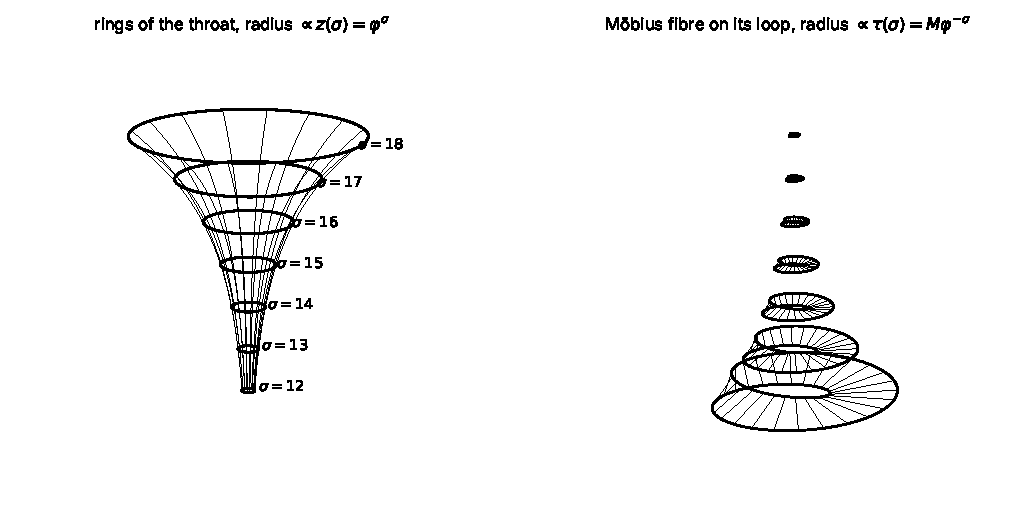
\includegraphics[width=0.80\textwidth]{fig_mobius_throat.pdf}
\caption{The two reciprocal families at the levels $\sigma=12,\dots,18$. Left: the rings of the
throat, radius $\propto z(\sigma)=\golden^{\sigma}$, growing upwards. Right: the M\"obius fibre on its
own loop, the half-turn period $\tau(\sigma)=M_{\mathrm{PCF}}\golden^{-\sigma}$, shrinking upwards;
on that loop the phase accumulates exactly $\varepsilon(\sigma)\tau(\sigma)=\pi$, a half-turn
\code{closure\_each\_level}, so the band is one-sided at every level. The product of the two radii is
the same at every level, $z\tau=M_{\mathrm{PCF}}$. The width of each band, half the radius of its
loop, draws the modulus $|\Omega|=\tfrac12$ of axiom~(B1); it is a convention of the drawing, since the
fibre is internal. Because the product is constant, the ring of level $\sigma$ holds $N=z/(\tau/M_{\mathrm{PCF}})=\golden^{2\sigma}=(S/\pi)^{2}$
loops \code{ring\_resolution\_is\_square}, never an integer \code{ring\_resolution\_irrational}: as
the throat grows and the loop shrinks, the ring is cut finer, as the square of its entropy, while
$\pi\sqrt N=S$ \code{cardy\_saturates\_bound}. The marks the loops lay on the ring are distributed
as in Figure~\ref{fig:granularity}; what $N$ and $S$ are physically is not said here.}\label{fig:mobius}
\medskip
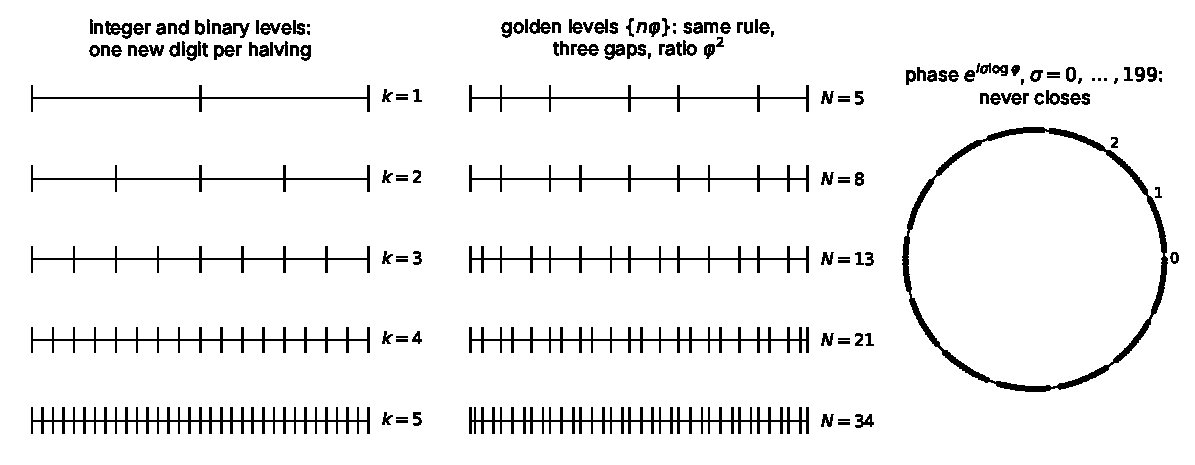
\includegraphics[width=0.92\textwidth]{fig_granularity.pdf}
\caption{Granularity. Left: integer and binary levels, $2^{k}$ cells need $k$ binary digits. Centre:
the golden levels $\{n\golden\}$ after $5,8,13,21,34$ points, refined by the additive rule alone; three gap
lengths, in the ratio $\golden$ and $\golden^{2}$, the largest shrinking by $\golden$ per Fibonacci
step. Right: the phase $e^{i\sigma\log\golden}$ for $\sigma=0,\dots,199$; it never closes, since
$\log\golden/\pi$ is irrational. The marks of the loops of Figure~\ref{fig:mobius} on the ring of level $\sigma$ are the same
construction at the rotation $1/N=\golden^{-2\sigma}$: at most three gap lengths, filling the ring
evenly. Against the left panel, the finer cut adds no new digit: the ring cut at the rotation $1/N$
carries $S=\pi\sqrt N$, not one digit per halving.}\label{fig:granularity}
\end{figure}

\begin{figure}[p]
\centering
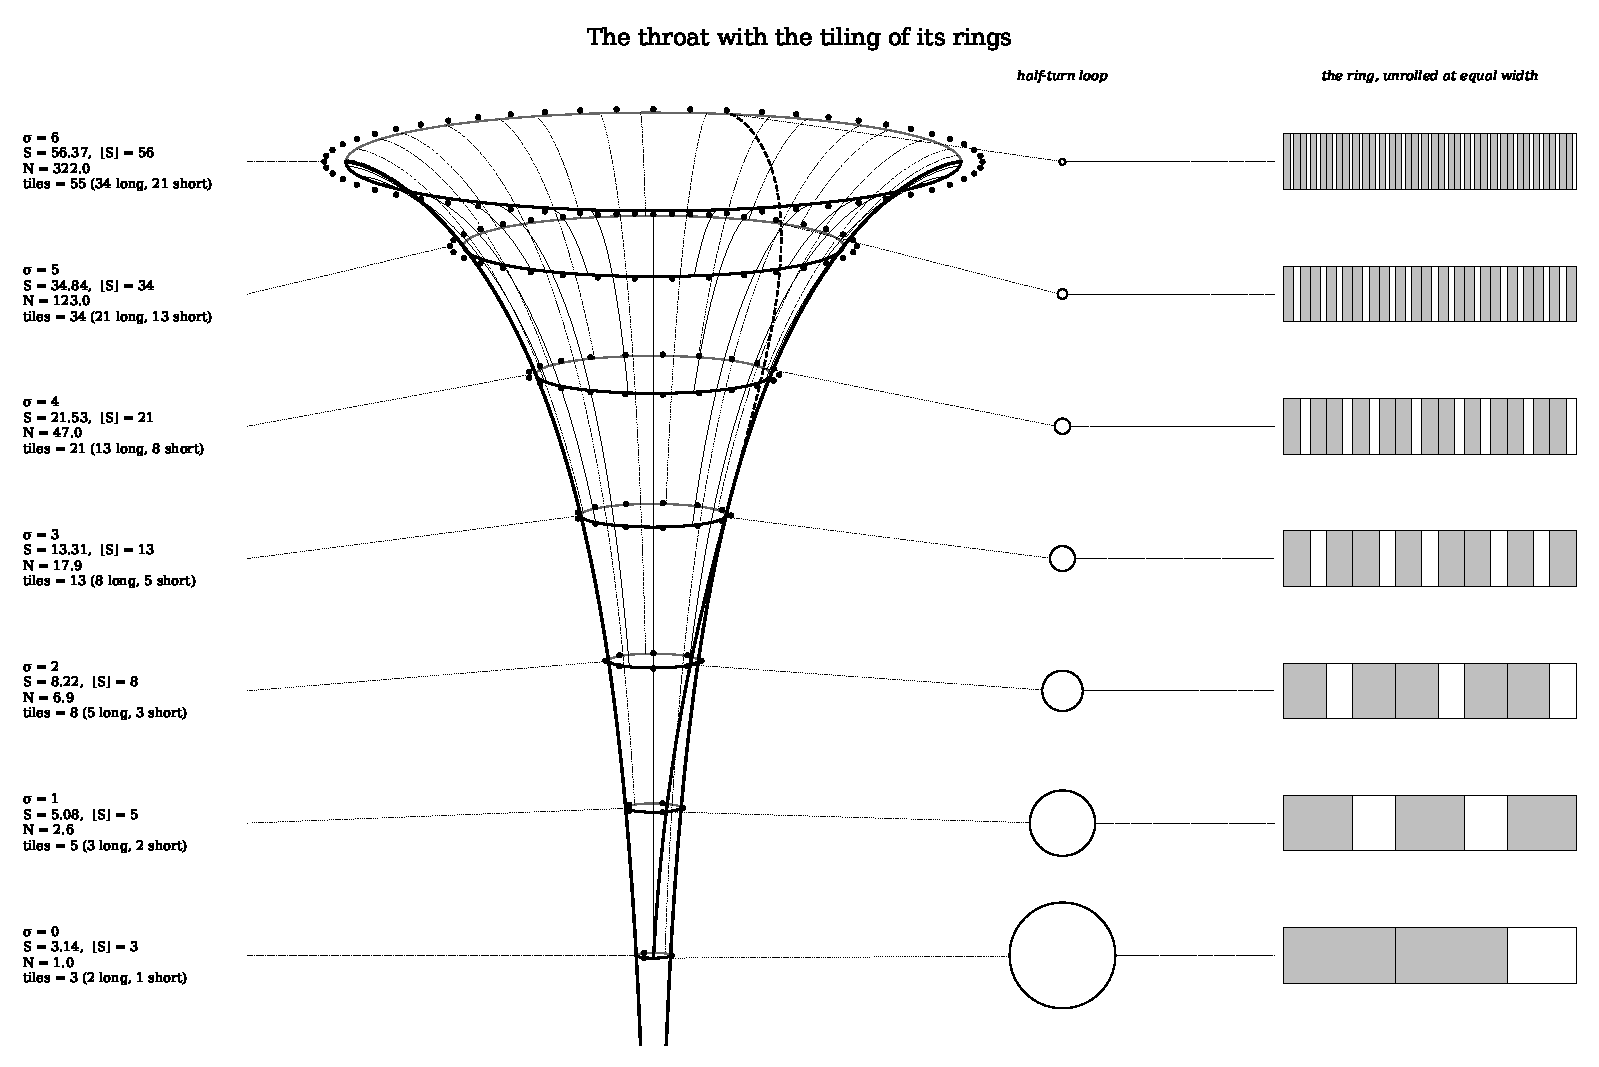
\includegraphics[width=0.9\textwidth]{fig_throat_tiling.pdf}
\caption{The throat of Figure~\ref{fig:background}(i), drawn at $\sigma=0,\dots,6$, with the tiling of its rings; by self-similarity the levels $12,\dots,18$ have the same form. Each band between two levels is cut by meridians into long and short tiles, whose arcs on a ring are in the ratio $\golden$; one level up a long tile becomes a long and a short one and a short tile a long one, so every boundary on a ring continues to the next, and the ring of each level is covered exactly by $A_\sigma$ long and $B_\sigma$ short tiles, $(2,1),(3,2),\dots,(34,21)$ \code{fibonacci\_substitution\_unique}. On the right each ring is unrolled at equal width, the long tiles shaded. Weighted by $1/(4G_N)=\tfrac12$ the tiles give $S(\sigma)=\pi(A_\sigma\golden^{-2}+B_\sigma\golden^{-3})$ exactly \code{two\_tile\_entropy}; their number, $F_{\sigma+4}=3,5,\dots,55$, is not $S$ and tends to $0.9757\,S$, while the dots are the $\lfloor S\rfloor$ modes, $3,5,\dots,56$. On the left, the numbers of each level; the thick line turns by $\log\golden$ per level and never closes (dashed behind the throat); in the middle column, the half-turn loop of each level, of radius $\propto\tau(\sigma)$, with $z\tau$ constant (Figure~\ref{fig:mobius}). Exact: the profile, the rings and their ratio $\golden$, the meridians of the tiles, the counts and the weights. Conventions of the drawing: the tilt of the view, the even spacing of the dots and the scale of the loops.}\label{fig:throattiling}
\end{figure}

\begin{figure}[p]
\vspace*{-1.5\baselineskip}
\begin{minipage}[t][\textheight][t]{\textwidth}
\centering
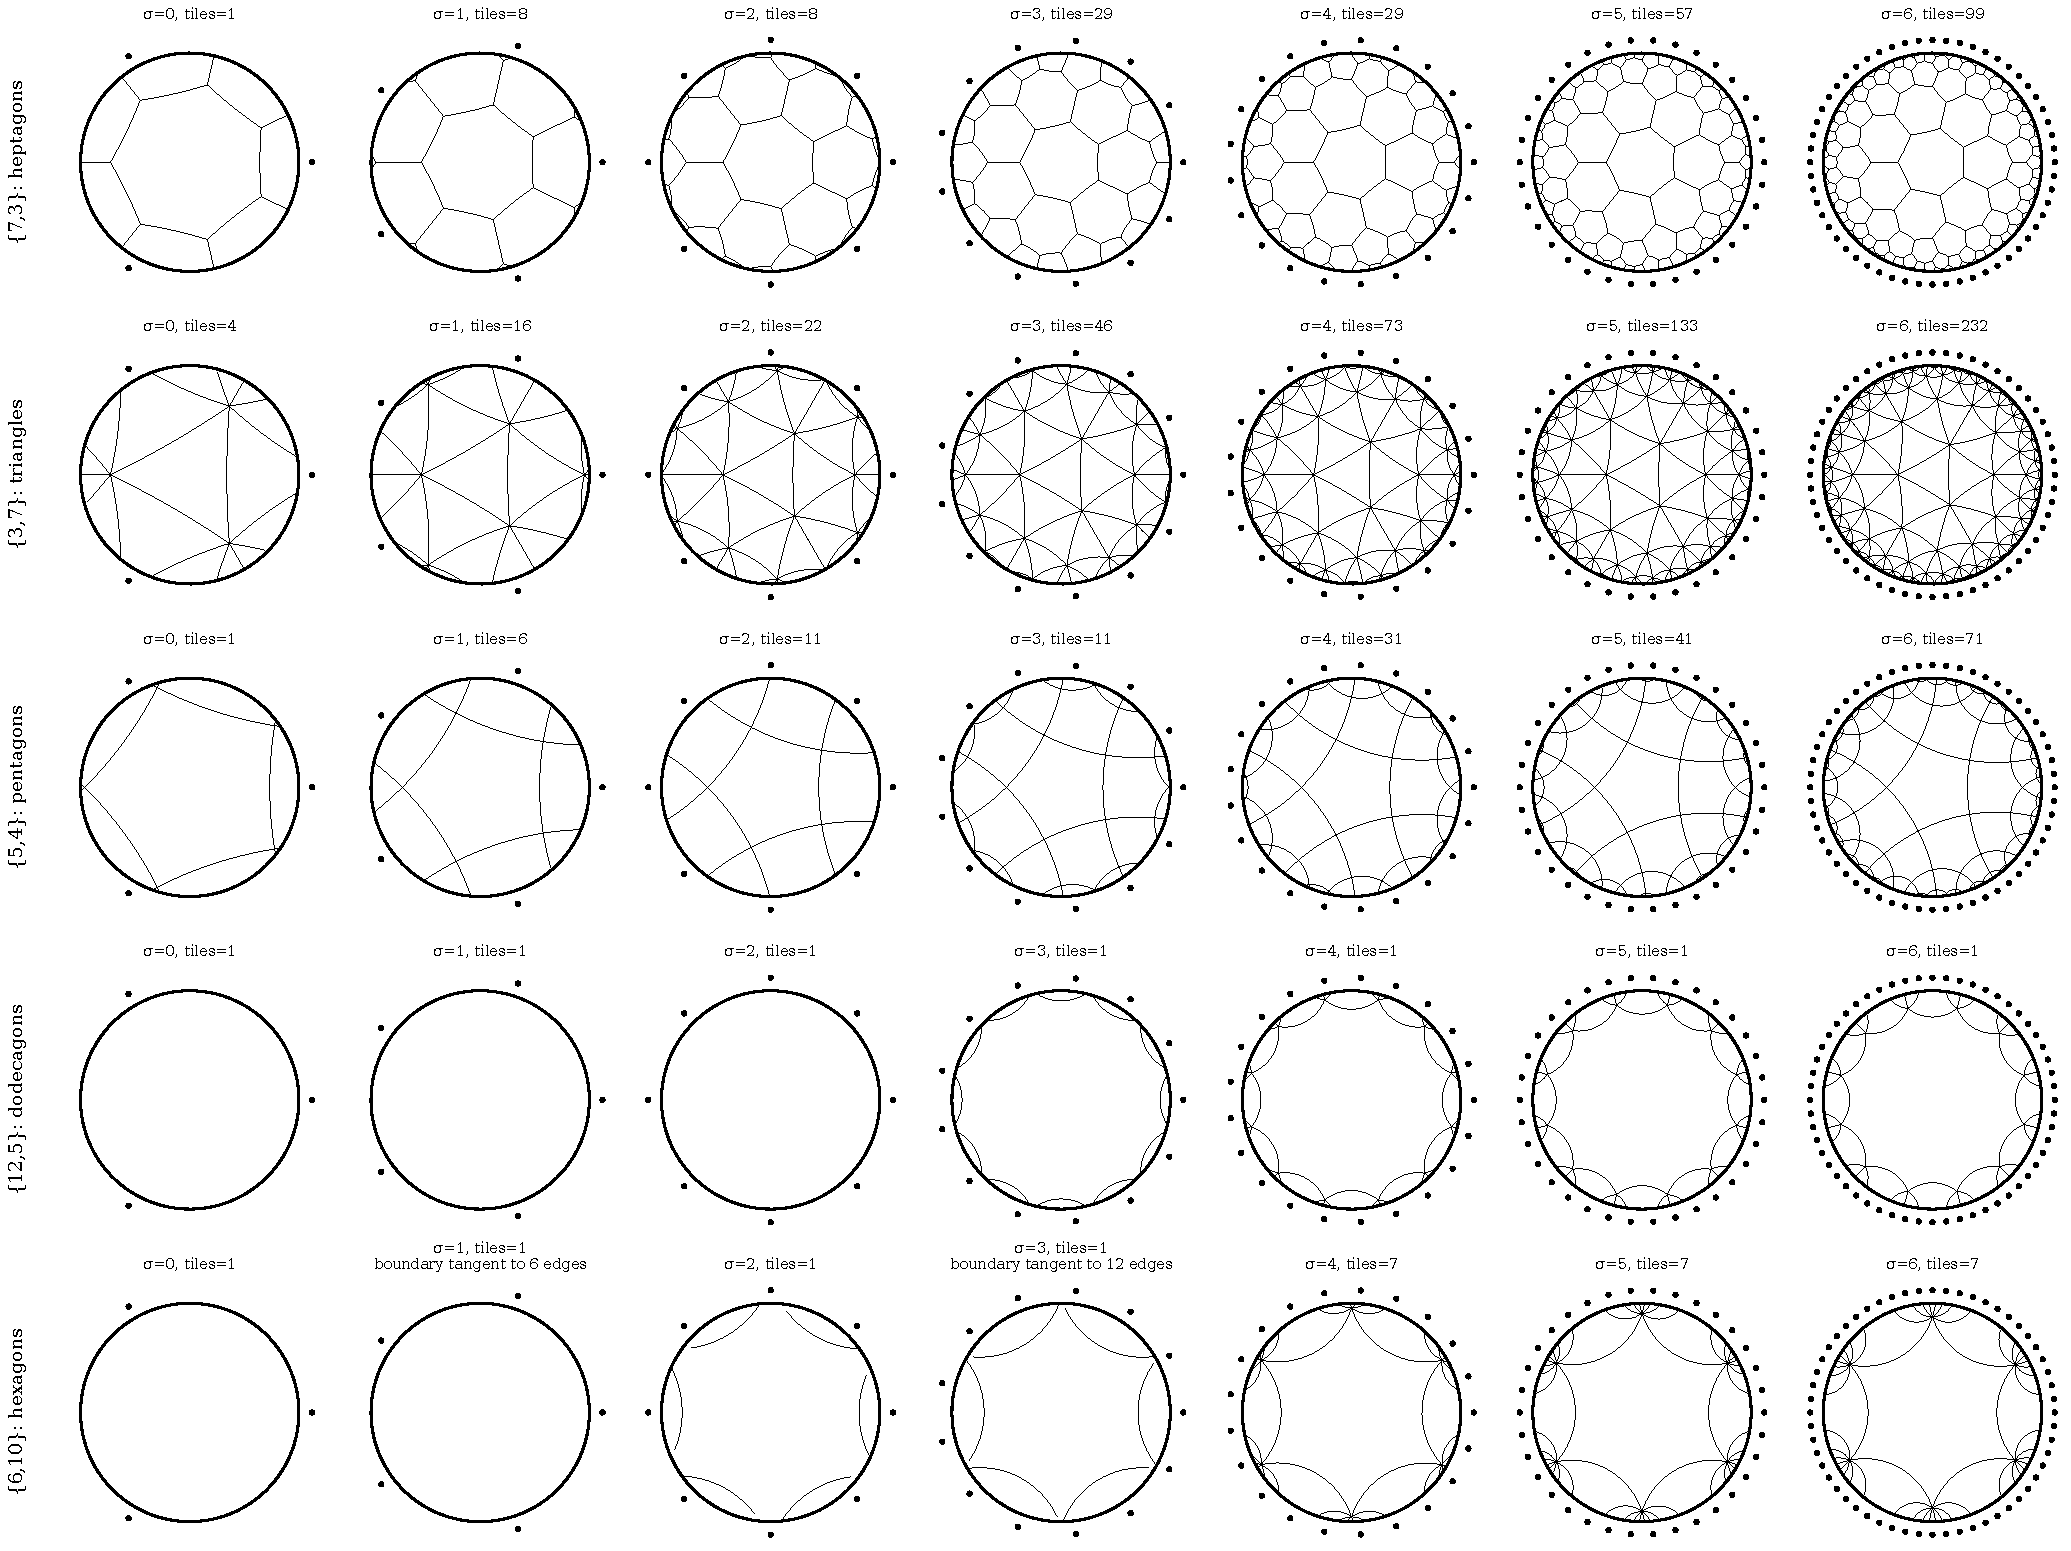
\includegraphics[width=\textwidth]{fig_tilings_strip.pdf}
\caption{Five regular tilings of the hyperbolic disk at the levels $\sigma=0,\dots,6$, each disk of radius $\operatorname{arsinh}z$ drawn at equal size, with the $\lfloor S\rfloor$ mode dots outside it: $\{7,3\}$, heptagons; $\{3,7\}$, triangles; $\{5,4\}$, pentagons; $\{12,5\}$, dodecagons; $\{6,10\}$, hexagons. Above each disk, the number of tiles whose centres lie inside it. In $\{12,5\}$ no tile but the central one has its centre inside a disk drawn, and the disks of $\sigma\le2$ lie inside that dodecagon, as those of $\sigma\le1$ lie inside the central hexagon of $\{6,10\}$, so they show no edge; in $\{6,10\}$ the boundary of the level touches edges at $\sigma=1$ and $\sigma=3$, and in no other tiling at any level drawn.
Why each is set aside, from what the code shows. $\{7,3\}$ grows by $\golden^{2}$ per layer, counted by edges and by vertices, but its centre has the order $7$, which none of the symmetries or clocks of the note has, and the edges that a level cuts give $S$ only on average, $2.41$ of them per unit of $S$ (\testref{test\_crofton\_constant}). $\{3,7\}$, the dual of $\{7,3\}$, has at its centre the order $3$ of $\rho$, and its layers grow by $\golden^{2}$ when taken by shared vertices but by about $1.6$ when taken by shared edges. $\{5,4\}$ comes closest: its edge is exact in $\golden$, $\cosh e=\golden$, its layers $5F_{2k}$ grow by $\golden^{2}$, its centre has the order $5$ and four tiles meet at each vertex, $4\cdot5=20$; it is the tiling of the pentagon code~\cite{PYHP15}, and with one qubit per bond it gives $1.49\,S$. $\{12,5\}$ carries $12\cdot5=60$, but grows by about $11$ per layer and has no length exact in $\golden$. $\{6,10\}$ carries $6\cdot10=60$ and its inscribed radius is exactly $\operatorname{arsinh}\golden$, the disk of $\sigma=1$, but it grows by about $5$ per layer. What would let one of them stand for the throat is a count that grows by exactly $\golden$ from one level to the next; a count is a whole number, its growth from level to level a fraction, and $\golden$ is not a fraction, so each gives $S$ only on average, and only with a bond dimension chosen to that end.
Used in \S\ref{ssec:math} and \S\ref{ssec:phys}.}\label{fig:tilingstrip}
\vfill
\end{minipage}
\end{figure}
% Both floats above are shorter than the 0.9\colht that amsart requires of a
% float page, so LaTeX defers them to \end{document} (they were landing after
% \printbibliography). Flushing them here puts them on their own float pages,
% where Figure~\ref{fig:throattiling} and Figure~\ref{fig:tilingstrip} are read.
\clearpage

The angular direction is the torus. The framework places the microstate on
$T^2=\mathbb{C}/M_{\mathrm{PCF}}\mathbb{Z}[i]$, $\tau=i$~\cite{CW6}, and the tower of lattices
$\golden^{\sigma}M_{\mathrm{PCF}}\mathbb{Z}[i]$ has $\tau=i$ at every level \tier[lattice\_tower\_tau]{P}:
the torus is the same at every level up to scale (Figure~\ref{fig:background}(a),(i)). The lattice points grow with the level: at the levels $\sigma=0,\dots,6$ of the tower of~\cite{CW6}, the points of $\mathbb{Z}[i]$ inside the ring of radius $\golden^{\sigma/2}$ are $5,5,9,13,21,37,57$. The disk has area $S(\sigma)=\pi\golden^{\sigma}$, the saturation entropy, and the count equals it only on average: the number of lattice points in a disk differs from its area by an error of lower order~\cite{Hux03}, and its ratio to $S$, $1.59,0.98,1.09,0.98,0.98,1.06,1.01$ here, is $0.9998$ at $\sigma=22$.
\witness{N}{\testref{test\_lattice\_points\_follow\_the\_area\_on\_average}, \testref{test\_ratio\_at\_sigma\_22\_is\_unity\_to\_four\_decimals}} The mode count, the circle count of \S\ref{sec:intro}, is $\lfloor S\rfloor=3,5,8,13,21,34,56$; at the bottom of the throat, $\sigma=12$, the lattice points are $1005$ and $\lfloor S(12)\rfloor=1011$ (\testref{test\_bottom\_of\_the\_throat}). The right angle of
the torus is not chosen. The microstate starts from the eigenvalue triangle $\tfrac12\omega^{k}$,
$\omega=e^{2\pi i/3}$, on a hexagonal lattice at $120^{\circ}$; the golden coupling $z=\golden y$,
a third direction tied to the plane by $\golden$, carries it onto the square lattice $\mathbb{Z}[i]$,
and $\tau=i$ is the fixed point of the quarter-turn $S$ that survives (Imported
statement~\ref{imp:coupling}). The third direction enters by isometry: seen along its diagonal, the cube $\mathbb Z^3$ projects each axis to $e_k-\tfrac13(1,1,1)$, of squared length $\tfrac23$ and at $120^{\circ}$ from the other two, onto a hexagonal lattice, $\mathbb Z[\omega]$ up to the factor $\sqrt{2/3}$; that projection has a kernel, the diagonal, since the three projected axes sum to zero \tier[cube\_diagonal\_kernel]{P}, whereas the golden coupling, a graph $z=\golden y$ over the plane, carries the third direction without one (\testref{test\_cube\_diagonal\_projection}). The torus is the
global object, the same at every level; the ring of each level is its local reading at that scale. A square torus has no isometric smooth image
in space, but it has an exact conformal one: the Clifford torus, whose two cycles have equal
length \tier[clifford\_square]{P}, projected stereographically, the torus of revolution with $R/r=\sqrt2$, $(\rho-\sqrt2)^2+z^2=1$
\tier[clifford\_stereographic\_torus]{P}; the projection is conformal on it, its induced metric being
$\rho^2(da^2+db^2)$ because $\rho'^2+z'^2=\rho^2$ \tier[stereographic\_meridian\_deriv, stereographic\_conformal]{P} (Figure~\ref{fig:background}(a)).

The two directions are tied by one quantity. The phase advances at the rate
$\varepsilon(\sigma)=\varepsilon_0\golden^{\sigma}$, which is the spectral angle,
$\tan\alpha(\sigma)=\varepsilon_0\golden^{\sigma}$ (Imported statement~\ref{imp:angle}), and over
the wavelength $\tau(\sigma)=M_{\mathrm{PCF}}\golden^{-\sigma}$ of Imported
statement~\ref{imp:lengths} it accumulates exactly a half-turn at every level,
$\varepsilon(\sigma)\tau(\sigma)=\varepsilon_0M_{\mathrm{PCF}}=\pi$ \tier[closure\_each\_level]{P}. The
half-turn is carried by the reciprocal length, not by the ring: over the ring $M_{\mathrm{PCF}}\golden^{\sigma}$
the phase is $\pi\golden^{2\sigma}$, a half-turn only at $\sigma=0$.
\witness{P}{phase\_on\_cell, phase\_on\_cell\_halfturn\_iff} This is the pair $z\tau=M_{\mathrm{PCF}}$ again:
the throat grows as the period of the half-turn shrinks. The accumulated phase $\pi$ acts on the
fibre, of modulus $\tfrac12$ at every phase \tier[worldline\_modulus]{P}, as $e^{i\pi}=-1$, of order
two \tier[fibre\_half\_turn]{P}; it is $\pi$ and not $2\pi$ because the modulus is $\tfrac12$
(Imported statement~\ref{imp:monodromy}): the fibre is a M\"obius band, one-sided~\cite[\S4.2]{CW6}. The loop
that carries the half-turn is the period $\tau(\sigma)$, which shrinks as the ring of the throat grows,
so the two are drawn side by side, each with its own radius, and their product is constant at every
level (Figure~\ref{fig:mobius}).

\emph{The ring is subdivided by the loop.} Because the product is constant, the number of loops of
the fibre that fit on the ring of a level is
\[
  N(\sigma)=\frac{z(\sigma)}{\tau(\sigma)/M_{\mathrm{PCF}}}=\golden^{2\sigma}=z(\sigma)^2=\Bigl(\frac{S(\sigma)}{\pi}\Bigr)^{2}
\]
\tier[ring\_resolution\_is\_square]{P}:
as the throat grows the loop shrinks, and the ring is cut finer, as the square of its radius and of
its entropy. $N(\sigma)$ is never an integer for any integer $\sigma\geq1$: writing
$\golden^{n+1}=F_{n+1}\golden+F_n$ with Fibonacci numbers, $\golden^{2\sigma}$ is irrational
\tier[golden\_pow\_fib, ring\_resolution\_irrational]{P}. So the half-turn marks laid along the ring, at
$k/N(\sigma)$ of a turn, never close on themselves; by the three-gap theorem~\cite{vRa88} they cut
the ring into at most three lengths, and by Weyl's theorem they fill it evenly. Numerically, for
$\sigma=1,\dots,6$ and up to $10^4$ marks, there are never more than three gap lengths and the
discrepancy stays below $0.005$
.
\witness{N}{\testref{test\_three\_gaps\_of\_the\_marks}, \testref{test\_discrepancy\_stays\_below\_half\_a\_percent}} The subdivision of the ring is the granularity of
Figure~\ref{fig:granularity} at the rotation $\golden^{-2\sigma}$. Two further identities are pure
algebra. With $c=3$ and $L_0=N/2$, Cardy's expression gives
$2\pi\sqrt{c L_0/6}=\pi\sqrt N=\pi\golden^{\sigma}=S(\sigma)$ \tier[cardy\_entropy, cardy\_is\_tower\_entropy]{P}~\cite{Car86}; and the closed-string mass
$m^2=(n/R)^2+(wR/\alpha')^2$ is invariant under $R\mapsto\alpha'/R$, $(n,w)\mapsto(w,n)$
\tier[closed\_string\_invariance]{P}~\cite{Pol98}, while with $\alpha'=M_{\mathrm{PCF}}$ the dual of the radius
$z(\sigma)$ is the loop $\tau(\sigma)$ \tier[dual\_radius\_is\_loop]{P}. Three comparisons of $N$ with
$S$ follow. First, $N$ exceeds $S$ from $\sigma=3$ on: $\golden^{3}=2+\sqrt5>\pi$
\tier[golden\_cube\_gt\_pi]{P}, so $\pi z<z^{2}$ for every $\sigma\geq3$.
\witness{P}{ring\_count\_exceeds\_bound, ring\_count\_exceeds\_bound\_from\_three} Second, the
expression $4\pi z^{2}/(4\cdot\tfrac12)=2\pi z^{2}$ equals $S=\pi z$ only at $z=\tfrac12$
\tier[area\_law\_4d\_meets\_weld\_iff]{P}, that is at $\sigma=-\log_\golden2$, below the bottom of the
tower. Third, $\pi\sqrt{N}=\pi z=S$ exactly \tier[cardy\_saturates\_bound]{P}, and the count behind
Cardy's expression can be done exactly: the number $W(L_0)$ of states at level $L_0$ of three free
bosons, the coefficient of $q^{L_0}$ in $\prod_{n\geq1}(1-q^{n})^{-3}$, gives at $L_0=\lfloor N/2\rceil$
\[
\begin{array}{c|ccc}
\sigma & 3 & 6 & 9\\\hline
\log W & 7.30 & 46.25 & 224.41\\
S=\pi\sqrt N & 13.33 & 56.37 & 238.80
\end{array}
\]
with ratio tending to $1$, and $S-\log W-\tfrac32\log L_0$ settling to a constant ($2.73$, $2.50$,
$2.44$), the logarithmic correction $(c+3)/4$ of Cardy's formula at $c=3$ \tier[\testref{test\_count\_against\_the\_entropy}]{N}. None of this
changes $S$, the masses or the lattice counts of the angular direction above.

This is why the bottom is a half-turn and the phase a quarter-turn: for the modular matrix $S$,
the half-turn is $S^2=-1$ and the quarter-turn is $S$ itself \tier[quarter\_and\_half\_turn]{P}. The same pair of turns acts on the three-sphere in which the square torus sits as the Clifford torus. The tori $|z_1|=\cos\eta$, $|z_2|=\sin\eta$ that foliate it are flat, of modulus $\tau=i\tan\eta$, and with $\tan\eta_n=\golden^{-2n}$ they are the tower of tori of the window, $\tau_n=i\golden^{-2n}$ of Imported statement~\ref{imp:gauss}, not the lattice torus of every level, whose modulus stays $\tau=i$; the two meet only at the level $0$, where the window torus is the Clifford torus.
\witness{P}{tan\_eta, level\_zero\_is\_clifford, clifford\_square} The exchange $z_1\leftrightarrow z_2$ is $\eta\mapsto\pi/2-\eta$, the mirror $n\mapsto-n$ of Imported statement~\ref{imp:gauss} \tier[swap\_is\_mirror, S\_acts\_as\_mirror]{P}, and each window torus projects stereographically, from a point of the circle $z_1=0$, onto a torus of revolution with $R/r=\sqrt{1+\golden^{4n}}$, $\sqrt2$ at the level $0$ \tier[stereo\_ratio, clifford\_stereographic\_torus]{P}. The map $J(z_1,z_2)=(-\bar z_2,\bar z_1)$, the quaternion $j$, has order four and square $-1$ \tier[J\_sq, J\_four]{P}: on the base of the Hopf fibration it is the antipodal map of W10 \tier[J\_lifts\_W10]{P}, on the tori it is the mirror \tier[J\_swaps\_moduli]{P}, and its square is the half-turn of the fibre, $-z=e^{i\pi}z$, which the base does not see \tier[antipode\_is\_half\_turn, hopf\_blind\_to\_half\_turn]{P} (\testref{test\_j\_squares\_to\_minus\_one\_and\_the\_half\_turn\_is\_invisible}). The antipodal map, the mirror and the half-turn are thus one quarter-turn and its square. The fibration itself is homogeneous: its isometries carry any fibre to any other; its tori are the preimages of the parallels of the base and need a chosen axis, which the same isometries carry to any other; the torus $\eta=\pi/4$ is fixed by the mirror, and the levels $\eta_n$ are placed by $\golden$ (Imported statement~\ref{imp:gauss}).
\witness{N}{\testref{test\_a\_torus\_is\_the\_preimage\_of\_a\_parallel\_and\_asks\_for\_an\_axis}, \testref{test\_the\_flat\_tori\_have\_modulus\_i\_tan\_eta}}

\begin{definition}[The hypertorus]\label{def:hypertorus}
The \emph{hypertorus} of the framework is the family, over the levels $\sigma$ of the throat, of
the torus $\mathbb{C}/\golden^{\sigma}M_{\mathrm{PCF}}\mathbb{Z}[i]$, $\tau=i$, carrying the M\"obius
fibre of modulus $\tfrac12$ whose half-turn period is $\tau(\sigma)=M_{\mathrm{PCF}}\golden^{-\sigma}$.
\end{definition}
\noindent Each of its three pieces is proved above: $\tau=i$ at every level
\tier[lattice\_tower\_tau]{P}, the half-turn at every level \tier[closure\_each\_level]{P}, and the
throat.
\witness{P}{pseudosphere\_unit\_speed, ring\_ratio} For a reader of AdS/CFT the difference with the usual throat is that the radial
direction is not integrated out to leave a boundary theory: bulk and boundary are kept, and the
boundary torus is the same at every level. The masses use only a minimal part of it: the measure,
the boundaries, the phase and the bottom.

\emph{The irrationality of $\golden$ acts twice.} In the usual constructions the levels are discrete: the Fourier modes
on a circle are $n/R$, and the Virasoro levels of the string are the integers of $L_0$~\cite{Pol98},
so a finer structure needs new generators, one more binary digit for each halving, a new register
for each refinement (Figure~\ref{fig:granularity}, left). Here the levels $\sigma$ are real: the
additive law holds for every real $\sigma$ (Imported statement~\ref{imp:additive}), and the second
generator is already enough. Because $\golden$ is irrational, $n\golden$ is never an integer for
$n\neq0$ \tier[golden\_irrational, golden\_rotation\_aperiodic]{P}, so the levels $a+b\golden$ never repeat, they are dense in the line, while a rational step $p/q$ would send the pair $(-p,q)$ to $0$, so that distinct pairs fall on one point, $14\,042$ coincidences among the pairs in $[-60,60]^2$ for $3/2$ against none for $\golden$ \tier[rational\_step\_kernel]{P} (\testref{test\_rational\_step\_has\_a\_kernel});
and by Weyl's theorem their fractional parts fill $[0,1)$ evenly~\cite{Wey16}. They refine under the same rule that builds the tower:
at $N=F_k$ points the largest gap is $\golden^{-(k-2)}$, one more Fibonacci step is one
more factor $\golden$, and no new dimension is added
\tier[\testref{test\_three\_golds\_with\_ratio\_phi\_squared}]{N}. Among irrational steps $\golden$ refines most
evenly: the first $N$ points cut the circle into at most three lengths~\cite{vRa88}, and for
$\golden$ their ratio is at most $\golden^{2}=2.618$, reached for every $N$ up to $5000$ except when
$N+1$, the marks with the origin, is a Fibonacci number, where only two lengths remain, in the ratio
$\golden$, against $3.414$ for
$\sqrt2$, $9.52$ for $e$ and $293.6$ for $\pi$ \tier[\testref{test\_worst\_gap\_ratio\_over\_the\_first\_5000\_levels}]{N} (Figure~\ref{fig:granularity}, centre); the
reason is the continued fraction $[1;1,1,\dots]$ of Imported statement~\ref{imp:polar}, which makes
$\golden$ the number least well approximated by fractions~\cite{Hur91}. The second irrationality is
that of $\golden$ with respect to $\pi$. Along the tower the phase of the worldline,
$e^{i\sigma\log\golden}$, turns by $\log\golden$ per level, and $\log\golden/\pi$ is irrational by the Gelfond--Schneider argument of \S\ref{sec:intro}~\cite{Sch35}. So the phase never closes and its values are dense on the circle (Figure~\ref{fig:granularity}, right). In the exact sense of Weyl's theorem one golden orbit does what an average
does: for every continuous function on the circle, its average along the orbit equals its average
over the circle~\cite{Wey16}; at each point of the orbit a product is the product, and along the
orbit the connected part $\langle fg\rangle-\langle f\rangle\langle g\rangle$ tends to
$\int fg-\int f\int g$.
\witness{P}{weyl\_equidistribution, orbit\_connected\_part, single\_theory\_factorizes} The connected term that item (e) of the proof after Imported
statement~\ref{imp:adscft} attributes to an average over several states is the one the orbit
produces: the average over a uniform family of phases is the average over the circle, so one orbit
gives, at each point, the factorisation of one state and, along itself, the connected part of an
average.

\emph{Discrete and continuous, in every dimension.} The levels are discrete and continuous at once:
discrete in how they are built, from pairs of integers $(a,b)$, and continuous in what they close
into, the dense set $a+b\golden$; one irrationality does both \tier[golden\_rotation\_aperiodic]{P}.
The string reaches density by adding: its Fourier modes and Virasoro levels form a lattice, and a
finer lattice needs more generators. Here density comes from the irrational ratio of two
generators, and in each dimension the framework uses, a contact arrangement of maximal size is given by
$\pi$ or by $\golden$. In one dimension a point has two neighbours, and the golden step spaces the
levels most evenly (three gaps, ratio $\golden^2$). In two the kissing number is $6$, attained by
the six units of $\mathbb{Z}[\omega]$, $\omega=e^{2\pi i/3}$, at distance $1$ from the origin and from
their neighbours \tier[hexagonal\_contact]{P}; this is the lattice of the eigenvalue triangle
$\tfrac12\omega^{k}$ of~\cite{CW6}, whose six minimal vectors are proved there
(\code{a2\_minimal\_vectors\_exactly\_six}), it is the side of $\pi$, and its packing is the
densest of the plane~\cite{FT40}. In three the kissing number is $12$~\cite{SvdW52}, and the
icosahedron attains it: its twelve vertices $(0,\pm1,\pm\golden)$ and their cyclic permutations lie
at squared distance $\golden+2$ from the centre, with neighbours at squared distance $4$
\tier[icosahedron\_vertex\_norm, icosahedron\_edges]{P}, so twelve unit spheres centred at distance $2$
touch the central one and do not meet each other, because $\golden+2<4$
\tier[icosahedral\_kissing]{P}; the face-centred cubic and hexagonal close-packed arrangements attain it as well, without $\golden$, and the icosahedron is the one among them in which $\golden$ is the coordinate. Here $\golden$ is the coordinate, the side of the scale, and it is
also the trace of the icosahedral rotation by $2\pi/5$, $1+2\cos(2\pi/5)=\golden$ \tier[golden\_is\_icosahedral\_trace]{P}. The
twelve of the icosahedron and the twelve of the bottom of the throat are proved separately: its
rotation group $A_5$ has order $60$, each vertex is fixed by the rotations of order $5$ about it,
so there are $60/5=12$ vertices \tier[twelve\_of\_the\_icosahedron]{P}; $60$ is also the clock of
$\golden$ modulo $10$, $\pi(10)=60=12\cdot5$ \tier[pisano\_orders]{P}, and $12=\operatorname{lcm}(4,6)=-1/\zeta(-1)$ is the
half-turn of Proposition~\ref{prop:twelve}~\cite{F1}, and that they are one twelve is a reading. Each vertex has five neighbours, the pentagon of $\golden=2\cos(\pi/5)$. \tier{N} for the full
list of distances (\testref{test\_icosaedral\_contact\_spheres\_do\_not\_touch}).

\emph{Real and integer: the lattice and its window.} The pairs $(a,b)$ that build the levels are
the points of a lattice, and the density of $a+b\golden$ is what that lattice looks like on one
line. With the second coordinate, the Galois conjugate, $\mathbb Z[\golden]$ is discrete in the
plane, and its units, the integer levels, lie on the hyperbola that a real level runs along
continuously (Imported statement~\ref{imp:units}): the hyperbola is the real face, which carries
the metric and the coordinate $y=\sigma\log\golden$; its lattice points are the integer face, which
carries what is counted, modes, bits and the clock. Projecting onto the first coordinate alone
loses which point is a lattice point; that loss is a loss of precision, not of generality. A
window on the second coordinate gives a cut-and-project set, the construction of the Fibonacci
quasicrystal~\cite{BG13,Jag21}; the tower is not that set but its points of norm $\pm1$, and the
weight on the second coordinate is not chosen: it is the self-dual Gaussian $e^{-\pi\bar x^2}$ of
Imported statement~\ref{imp:gauss}, a weight and not a window. Two spaces can carry it. On the index $\sigma=a+b\golden$ the integer $12$ has conjugate $12$ and weight $e^{-144\pi}$,
about $10^{-196}$, and the observed bottom would sit at $4+5\golden=12.09$: that form contradicts
the clock and is eliminated.
\witness{N}{\testref{test\_the\_integer\_12\_kills\_the\_cut}, \testref{test\_best\_lattice\_index}} On the scale $\golden^{\sigma}$ the unit $\golden^n$ has conjugate
$\pm\golden^{-n}$ and weight $w(n)=e^{-\pi\golden^{-2n}}$, which with the norm $\pm1$ gives the tower
itself; $w(n)>\tfrac12$ if and only if $\pi\golden^{-2n}<\log2$ \tier[window\_half\_iff]{P}, and since
$\pi/\golden^2>\log2>\pi/\golden^4$, the first integer level that passes
the threshold $\tfrac12$ of W1 is $n=2$, for every threshold between $0.301$ and $0.632$ \tier[\testref{test\_first\_active\_level\_is\_two}]{N}.
The first integer level whose Hubble rate is below the inverse bulk radius, $H_{\mathrm{dS}}(n)\ell<1$, is also
$n=2$, since $2/\golden>1>2/\golden^2$. The level at which~\cite{CW6}
places gravity, $\sigma_G=2$, the arity less one, is thus reached by two further routes, a window and
a radius. The two are distinct conditions on the same variable, one on the self-dual width $\pi$ with
the threshold $\log2$, the other on the factor $2$ of the Hubble rate, and neither follows from the
other; the route of the arity is of another kind. The set and the tower are one lattice read twice: the ring of level $\sigma$ of Figure~\ref{fig:throattiling}, with $F_{\sigma+3}$ long and $F_{\sigma+2}$ short tiles, is labelled by the unit $\golden^{\sigma+3}=F_{\sigma+2}+F_{\sigma+3}\golden$ \tier[golden\_pow\_fib]{P}, and its word of tiles is a periodic approximant of the cut-and-project set (\testref{test\_ring\_word\_is\_the\_fibonacci\_rotations}). The Fourier transform of that set is a sum of Bragg peaks on the module $(\mathbb Z+\mathbb Z\golden)/(\golden+2)$, with amplitudes $0.95$, $0.88$ and $0.70$ at $(m,n)=(2,3),(1,2),(1,1)$ for $46\,368$ tiles, against at most $0.010$ at points chosen at random.
\witness{N}{\testref{test\_bragg\_peaks\_of\_the\_fibonacci\_chain}, \testref{test\_bragg\_random\_level}}

\emph{The three columns.} Read through the Rosetta stone, the pieces above are one translation. The unit $\golden^{\sigma}$ on the line is the arithmetic column; its pair with the conjugate on the plane of Imported statement~\ref{imp:units}, with the horocycle of the cusp and the lattice $\mathbb Z[i]$ of the torus, is arithmetic geometry; and the third direction enters by isometry through the golden coupling. The torus $\mathbb C/M_{\mathrm{PCF}}\mathbb Z[i]$ is a Riemann surface, Weil's third column; the second has no counterpart over a finite field here beyond the Pisano periods of Imported statement~\ref{imp:clocks}, so the three columns are a comparison of form. The throat meets the conditions of \S\ref{sec:discussion} by facts proved above, which is how they were read: the translation is invertible on what is counted, because $\golden$ is irrational and the step of level is unimodular \tier[golden\_rotation\_aperiodic, level\_step\_is\_exchange\_shift]{P}; the same at every level, by the additive law (Imported statement~\ref{imp:additive}); and exact at each level, by the two weights, with the unweighted count within $\golden^{-(\sigma+4)}/\sqrt5$ of its mean.

\emph{The quarter-turn and the scale.} Read through Imported statement~\ref{imp:gauss}, the window
is the nome of a torus of modulus $\tau_n=i/N(n)$ at each level, and the tower of levels is a tower of
tori that degenerate towards the cusp: this is, in mathematics, the shrinking of the compactification,
the ring of level $n$ being cut into $N(n)=\golden^{2n}$ cells by the loops of the M\"obius fibre. The
quarter-turn $S$ of the clock acts on that tower as the Galois mirror of the scale
\tier[S\_acts\_as\_mirror]{P}, so the fractions of the clock, the half-turn of the monodromy and the
quarter-turn of $S$, and the step $\golden$ of the scale are one involution read in two variables. The
weight $\tfrac12$ is crossed at $n_{1/2}=\tfrac12\log_\golden(\pi/\log2)=1.570247$, against the
quarter-turn $\pi/2=1.570796$, and $w(\pi/2)=0.50018$ \tier[\testref{test\_weight\_crossing\_is\_a\_quarter\_turn}]{N}. The crossing is not exactly the
quarter-turn: it would be for a width $\log2\cdot\golden^{\pi}=3.1433$, and the self-dual width is $\pi$,
fixed by three conditions; what is exact is the structure that joins them, the action of $S$ on the
tower. At the level $0$, $\tau=i$, the window meets the lemniscatic value of Imported
statement~\ref{imp:gauss}, with the $\Gamma$ of the quarter.

\emph{The mirror-invariant interval and the two scales.} An interval of levels that the mirror leaves
invariant is symmetric about $0$ \tier[invariant\_interval\_symmetric]{P}; the one that joins the bottom
to its mirror image is $[-12,12]$, centred on the self-dual point of the two lengths of Imported
statement~\ref{imp:lengths} and of length $24$, the clock \tier[symmetric\_throat\_is\_clock]{P}. The two
coordinates of a unit carry the two scales of a level: the Kaluza--Klein scale $m_0\golden^{\sigma}$ on
the first and $H_{\mathrm{dS}}(\sigma)^2/2=\golden^{-\sigma}$ on the mirror, and their product is the norm,
$m_0\golden^{\sigma}\cdot H_{\mathrm{dS}}(\sigma)^2/2=m_0$ at every level \tier[kk\_hubble\_norm]{P}; an integer
level of the first is an even level of the second \tier[mass\_level\_even\_curvature]{P}, and $2$, the factor
between $G_N=\tfrac12$ and $G_N=1$, is not a unit, of norm $4$ \tier[two\_not\_unit]{P}.

\emph{The modulus of the ring and its metric.} The torus of modulus $\tau_n$ has the standard metric of
its complex structure, from $K=-\log(2\,\mathrm{Im}\,\tau)$, $K_{\tau\bar\tau}=1/(4(\mathrm{Im}\,\tau)^2)$:
for $\tau=it$ the kinetic term is $(\partial t)^2/(4t^2)=\tfrac12(\partial\Phi)^2$ with
$\Phi=\log t/\sqrt2$, so $d\Phi/dn=\sqrt2\log\golden$, and a potential $V\propto\golden^{-n}$ has
$|\partial_\Phi V|/V=\log\golden/(\sqrt2\log\golden)=1/\sqrt2$ \tier[moduli\_slope]{P}, under the
stated assumptions that the level $n$ of the window is the level $\sigma$ of the ladder and that the
modulus is that of complex structure with $M_{\mathrm{Pl}}=1$.

\emph{One dimensionless number.} With $\hbar$, $c$, $M$ and $G$ there is one dimensionless group,
$GM^2/\hbar c=(M/M_{\mathrm{Pl}})^2$, by the $\Pi$ theorem~\cite{Buc14}: the relation the framework lacks
between its two dimensionful data is one number, $\log_\golden(M_{\mathrm{Pl}}/M)=93.737$ \tier[\testref{test\_uv\_level}]{N}, and
its equality with the position of the top is the definition of \S\ref{sec:prediction}, not a theorem.

\emph{The level, the phase and the bottom.} Four identities tie the tower to the criteria of
\S\ref{sec:inputs}. First, $\Lambda(\sigma)S(\sigma)=6\pi$ at every level \tier[lambda\_times\_entropy]{P}:
the product of the two quantities of the weld is invariant along the flow of levels. Second, the
asymptotic phase of the zeros of $J_{d/2-1}$, which are the masses for a bulk of dimension $d+1$, is
$d/4-\tfrac34$, and it equals $1/d$ if and only if $d=4$, since $(d-4)(d+1)=0$
\tier[phase\_equals\_inverse\_dimension\_iff]{P}: the quarter of the tower is $|\Omega|^2=1/(n+1)$ and no
other dimension makes it so. Third, the zero mode is the exact term $k=0$: $J_1(0)=0$
\tier[bessel\_zero\_mode]{P}, where the asymptotic form would give $\pi/4$
\tier[zero\_mode\_vs\_asymptotic]{P}; the deviation of the exact zeros from it is largest there and
falls after, $j_{1,k}/\pi-k=0.2197,0.2331,0.2383,\dots\to\tfrac14$
\tier[\testref{test\_offsets\_against\_the\_printed\_column}]{N}. Fourth, the bottom is
twice the ceiling of W8, $12=2\sigma_\Lambda=2|\Lambda_5|=(n+1)n$, and $n(n+1)=4n$ if and only if
$n=3$ \tier[bottom\_twice\_lambda\_iff]{P}. The theta series obeys the law under $S$,
$\vartheta(-1/\tau)=(-i\tau)^{1/2}\vartheta(\tau)$, by Mathlib \tier[theta\_S\_law]{P}, with no axiom;
the law of $\eta$ under $S$ remains a classical input. The flow $\sigma\mapsto\sigma+t$ is homogeneous,
$\Lambda S$ being invariant along it; the clock breaks that homogeneity at one point, the half-turn
$12$ of Proposition~\ref{prop:twelve}, and that point is where the bottom sits.

\subsection{The physical retroduction: what the structure represents}\label{ssec:phys}

This part says what the structure of \S\ref{ssec:math} represents. Its claims are identifications
of mathematical objects with physical ones, the axioms (B) read on their physical side and the
axioms (F); each is marked where it is made, and which of them the data test is said in \S\ref{sec:inputs}.

\emph{The fifth dimension.} In~\cite{RS99} the extra dimension is postulated, and with it $k$,
$k\pi r$ and $d$. Here it is the tower of the framework, the levels $\sigma$ of its scale operator,
and its metric is not postulated: it is the measure that reflection positivity imposes on the
tower operator. The equations coincide (Proposition~\ref{prop:rs}); the origin differs. The
continuum of the two-brane model is the golden grid refined, and the levels carry the geometry,
not the modes (Remark~\ref{rmk:levels}). The tower is open because it is spectral: closing it into
a ring makes the transfer hyperbolic and the spectrum complex (Remark~\ref{rmk:bloch}). Read through the translation of \S\ref{ssec:math}, its compact direction is the fibre, whose period $\tau(\sigma)$ is the internal coordinate of the level (Imported statement~\ref{imp:units}): it shrinks because $\golden$ is a Pisot unit while the entropy grows in the physical coordinate, and their product is constant because the norm is a unit, so that the passage between them loses nothing; the sign of the norm, $(-1)^{\sigma}$, alternates as the half-turn does from level to level, $\varepsilon(\sigma)\tau(\sigma)=\pi$ \tier[closure\_each\_level]{P}. The dimensions follow the columns: in one, the line of energies, the spectrum of the tower; in two, the ring with its time, where the boundary theory of $c=3$ lives (Imported statement~\ref{imp:adscft}); in three, the section with its time, the bulk that the isometry $V^\dagger V=\mathbf 1$ keeps on that boundary \tier[bulk\_boundary\_isometry]{P}; in four, Minkowski space, where the Kaluza--Klein modes are particles; in five, the throat, whose step $\log\golden$ is the regulator of $\mathbb Z[\golden]$ (read through \S\ref{ssec:math}).

\emph{What each side chooses and the other fixes.} At the level of the equations,
\begin{center}\small
\begin{tabular}{@{}ll@{}}
\toprule
two-brane model & golden throat \\
\midrule
warp $e^{-ky}$ & $\golden^{\sigma-\sigma_{\mathrm{UV}}}$ \\
Kaluza--Klein scale $k\,e^{-k\pi r}$ & $H(\sigma_{\mathrm{IR}})=m_0\golden^{\sigma_{\mathrm{IR}}}$ \\
depth $k\pi r$ & $(\sigma_{\mathrm{UV}}-\sigma_{\mathrm{IR}})\log\golden$ \\
$d=4$, assumed & $d=n+1$, from the arity \\
infrared scale, fitted & $\sigma_{\mathrm{IR}}=-1/\zeta(-1)$ \\
\bottomrule
\end{tabular}
\end{center}
Read with the two-brane model, the data of~\cite{LYR26} fit a free scale; read with the framework,
they point to a level. The one quantity free on both sides is the position of the ultraviolet end.

\emph{From a choice among vacua to one theory.} The construction does not select one theory from a
space of choices by measurement; it closes that space by overdetermination. Each of the four conditions
fixes one element of the spectrum, the measure, the boundaries and weight, the phase and the bottom;
the first three agree on $d=4$, which the measure carries as its exponent and the phase as its
offset, and the fourth is independent of them. Outside the tower the dimension is fixed once more: the constant of the first de~Sitter patch, $\Lambda(0)=3/G_N$ by the entropy law of W4 with $S(0)=\pi$, and that of the throat, $|\Lambda_5|=d(d-1)/2$ (W8), agree only at $d=4$ with $G_N=\tfrac12$ \tier[dS\_entropy\_law, two\_routes\_to\_six]{P}; with the patch and the throat taken in the same dimension, $d=4$ is the only integer at which they agree (\testref{test\_only\_four\_dimensions\_share\_the\_two\_constants}). Together the four conditions leave one tower, up to the position of its top. Why one tower can stand where a choice stood, of a vacuum, of a value of the parameters of the baby
universes or of a boundary theory to average over (\S\ref{sec:intro}), is the pair of irrationalities
proved in \S\ref{ssec:math}. The two irrationalities are the granularity that either ensemble supplies
by multiplying theories: levels as fine as wanted, by one rule, and phases that cover the whole
circle, on one torus. The correspondence itself needs no choice: it holds from one microstate at every level, and one
state factorises (Imported statement~\ref{imp:adscft}, items (a) and (e) of its proof).
Where~\cite{MM20} place each value of the parameters in a superselection sector that is one theory and
factorises, here one state does; and the connected part that in the average is carried by spacetime
wormholes~\cite{MM20,SSSY24} is here produced along the orbit of the phase of the tower, of irrational step $\log\golden/2\pi$
(\S\ref{ssec:math}). Both are
comparisons of form (\S\ref{ssec:math}). What an ensemble adds beyond the envelope, the statistics
of its level spacings, is a statement about fluctuations (Imported statement~\ref{imp:envelope}). For
the Kaluza--Klein tower the operator gives those too: Theorem~\ref{thm:bessel} fixes every level, so
the fluctuations around the envelope are fixed with it, and their statistics is rigidity, spacings
falling to $\pi$, which the data show against the ensemble value (\S\ref{sec:arity}).

\emph{The dictionary without a choice.} The further choice of \S\ref{sec:intro}, that of a discretisation, can be put to numbers. A network on a regular tiling cut at the level $\sigma$ has as many open legs as edges the boundary of the level crosses; by Crofton's formula~\cite{San76} their number is, on average, a constant of the tiling times the length of the boundary, so their entropy is $S$ only on average and only for a bond dimension $\chi$ chosen to that end. For $\{7,3\}$ the ratio of the legs to $S$ runs $2.23,2.75,3.40,\dots,2.42$ over $\sigma=0,\dots,12$, about its constant $2.41$; of the $50\,340$ pairs of a tiling with $p,q\le60$ and an integer $\chi\le16$, $172$ give $S$ on average within $1\%$, none exactly, and the best, $\{20,3\}$ with $\chi=3$, within $3\times10^{-6}$, which no larger search improves
\tier[\testref{test\_pairs\_that\_give\_s\_on\_average}]{N}. Choosing that pair, or any other, is a selection by the number it must match, the place that the vacuum holds in the landscape~\cite{BP00,Wei87}, as choosing a radius is for the modes $n/R$ of a string; both read the golden lattice through rational ratios (\S\ref{ssec:math}). In the throat the dictionary is the area law itself, and its weight is not fitted to $S$: $1/(4G_N)=\tfrac12$ is the modulus $|\Omega|=\tfrac12$ of the microstate, the fixed point of $x\mapsto1-x$ (\S\ref{sec:inputs}), identified with $G_N$ (Imported statement~\ref{imp:adscft}, item (d)) \tier[area\_quantum\_half]{P}. $S(\sigma)$ is written with the same $G_N$, so that the weight and the entropy agree is the consistency of that identification, not a contrast. The contrast is elsewhere: the network fits $\chi$ to $S$ and then gives $S$ only on average, its legs fluctuating from level to level about a constant of the tiling; the throat sets $G_N$ by the identification before, and with the two fixed weights of \S\ref{ssec:math} gives $S$ at every level. In a network the cut is counted in bonds and no string appears; in the throat the cut is the closed string itself: the ring of the level, the circle that the string winds by (F6), has length $2\pi\golden^{\sigma}$ and carries $\tfrac12$ per unit of length (\S\ref{ssec:math}), so that $S$ is the length of the string times $1/(4G_N)$ where the network has the number of bonds times $\log\chi$. The tensor of the throat is the triad $V$ of Imported statement~\ref{imp:adscft}, one leg of dimension three, where a holographic code is built from perfect tensors of several legs~\cite{PYHP15}. The tiles are not qudits: a long tile would need a bond of dimension $e^{\pi/\golden^{2}}=3.32$ and a short one $e^{\pi/\golden^{3}}=2.10$, so the throat gives an area counted by two weights and not a network of integer bonds, whose Hilbert space would be a tensor product over the bonds, of dimension $\chi^{n}$; the dimension of a level is the integer of W2, and its growth $e^{S}$ is not $\chi^{n}$ for any integer $\chi$ at any integer level, since $e^{S/n}=(-1)^{-i\golden^{\sigma}/n}$ is transcendental by the Gelfond--Schneider theorem~\cite{Sch35} \tier[level\_growth\_not\_power]{P}. The discretisation of the dictionary therefore adds no choice to the tower for $S$: what the network selects to match $S$, the structure fixes (\testref{test\_pairs\_that\_give\_s\_on\_average}).


\emph{The level of the observer and the lattice.} Read with axiom~(F8), the level of the observer's
patch is read from the observed universe. In the gravitational unit $\ell=\sqrt2\,\ell_P$ the curvature
$\Lambda(\sigma)=6\golden^{-\sigma}$ and the entropy $S(\sigma)=\pi\golden^{\sigma}$ give the same level,
since $\Lambda S=6\pi$ (W4, W9): with $S_{\mathrm{obs}}=3\pi/(\Lambda_{\mathrm{obs}}\ell_P^2)=3.3\times10^{122}$
and the Planck values of \S\ref{sec:data}, $\sigma_{\mathrm{obs}}=583.88\pm0.04$, and $583.40$ with
the local $H_0$ \tier[\testref{test\_data\_readings}]{N}. The same curvature measured in the unit $u$ of (F1) reads $380.31$; the
difference, $2\log_\golden(M_{\mathrm{Pl}}/u)-\log_\golden2=203.56$, is the conversion between the two
units and not a second position. The value $585.3$ of~\cite{CW6}, eq.~(sigma-obs), takes $\Lambda$ in
$\ell_P$ with the $6$ of $G_N=\tfrac12$; with the unit to which $G_N=\tfrac12$ is relative it is $583.88$. The level so read with the Planck values is that of the asymptotic de~Sitter state, which $\Lambda_{\mathrm{obs}}$ alone defines; with the same values the level of today's Hubble horizon, with $H_0$ in place of $H_0\Omega_\Lambda^{1/2}$, is $583.09$, below it, and rises towards it as the universe expands (\S\ref{sec:data}) \tier[\testref{test\_the\_asymptotic\_and\_today\_levels\_are\_the\_printed\_two}]{N}. The level read is therefore the asymptotic level of the horizon, the most an observer can accumulate: with $G_N=\tfrac12$, $S_{\mathrm{obs}}$ is the $N$-bound $3\pi/(\Lambda G_N)$ that Bousso places on the observable entropy of every universe with $\Lambda>0$~\cite{Bou00}, the logarithm of the finite number of states of~\cite{Ban01}, and the entropy of the state of maximum entropy of the algebra of the patch~\cite{CLPW23}.

The integer levels are the units of $\mathbb Z[\golden]$ (Imported statement~\ref{imp:units}), and
the hypothesis that the observer's patch sits at one of them, a lattice point, was put to the data
with this criterion: it is excluded if the level read from the $\Lambda$CDM
determination of $\Omega_\Lambda h^2=(1-\Omega_m)h^2$ from the cosmic microwave background and the
baryon acoustic oscillations lies three standard deviations or more from every integer. The
contrast is with the nearest integer, not with a level named in advance; it is made within
$\Lambda$CDM because (F8) gives each level a constant. The points $583$, $584$ and $585$ require
$\Omega_\Lambda h^2=0.4737$, $0.2928$ and $0.1809$, a factor $\golden$ apart. The determination of
\S\ref{sec:data} gives $\Omega_\Lambda h^2=0.3240\pm0.0043$ with the published correlation, and the
level $583.789\pm0.028$, $7.6$ standard deviations from $584$; for every correlation between $-1$ and $1$ the
distance is at least $7.6$, reached at $-1$, and without the correlation it would be $10.5$, so the
result does not depend on it. Planck alone gives $583.877$, $2.2$ to
$3.1$ standard deviations from $584$ as the correlation of $\Omega_m$ and $H_0$ runs from $-1$ to
$0$; the local $H_0$ with the $\omega_m$ of Planck, a combination that $\Lambda$CDM does not
reconcile, gives $583.40$, nearest to $583$ and $5.0$ standard deviations from it.
\witness{N}{\testref{test\_data\_readings}, \testref{test\_the\_planck\_level\_is\_2\_2\_to\_3\_1\_sigma\_from\_584}} The
hypothesis is therefore excluded, by the criterion stated in advance, and the other determinations do not undo it: Planck alone agrees with the combination, $1.4$ to $1.8$ standard deviations from it in $\Omega_\Lambda h^2$, and differs only in precision, so it does not favour $584$ (\testref{test\_desi\_against\_planck}); the local $H_0$ moves the nearest integer to $583$ and excludes that one \tier[\testref{test\_the\_worst\_case\_is\_deci}]{N}. A tower with a rational step $p/q$ in place of $\golden$ reads the same data at other levels: with $21/13$ the bottom moves by $0.8$ standard deviations, which the data of \S\ref{sec:data} do not exclude, and the observer's level by $71$ (\testref{test\_rational\_step\_versus\_the\_contrast}); it stays within three standard deviations of the golden reading only from $144/89$ on, and each further depth asks for the next fraction, the convergents of $\golden$. This compares the steps with each other, not with a datum: what singles out $\golden$ is the clock and the additive law, not the data \tier[\testref{test\_three\_sigma\_criterion}]{N}. No measurement error is known that would remove the exclusion, the unit is
fixed by an argument independent of the data and cannot be moved, and no level of the structure
singles out $584$ ($584\equiv8\bmod 24$), so there is no mechanism to protect. An evolving dark
energy would change the form of (F8), not this contrast. The exclusion leaves the rest in
place: no mass depends on it, and the observer is read on the tower at a real level, which the
tower has, since a real level runs along the hyperbola on which the lattice points lie. Why the level
read is not an integer is a question the note keeps. The structure gives the finite Hilbert space of
a level, of entropy $S(\sigma)$ and $\lfloor S(\sigma)\rfloor$ modes at every real $\sigma$ (W2),
as~\cite{Wit01} requires,
and the datum gives the level, as in the view that $\Lambda$ is an input~\cite{Ban01}. This is the
note's answer to the cosmological form of the question of \S\ref{sec:intro}, in which the parameters
of the baby universes fix $\Lambda$: here $\Lambda$ is neither chosen nor fixed but read, and the
lattice form that would have fixed it is excluded. The note does not fix $\Lambda$: it reads its level, and what it
contrasts with $\Lambda$ is the lattice form of that level.

What places the observer there is, in~\cite{CW6}, accumulation and not selection, and both words have a precise content. The observer is localised information: the projection of W1, internal and with no region outside, read at the centre of the throat, whose modulus $\tfrac12$ is carried from the non-local type~III field to the particle that emerges from its tension~\cite[\S4.2]{CW6}. What it can ever reach is exactly half of de~Sitter space: the planar patch, $X_0+X_4=\ell e^{t/\ell}>0$, is the causal future of its worldline and covers one of the two halves of the hyperboloid that the antipodal map of W10 exchanges in~\cite{CW6} \tier[planar\_patch\_positive]{P}; what it can ever receive is the other planar patch, $X_4-X_0>0$, and the two meet in its static patch, a quarter \tier[\testref{test\_the\_static\_patch\_is\_a\_quarter}]{N}. The other half is not outside but antipodal, and that the half it reaches is the modulus $\tfrac12$ is the identification of~\cite{CW6}. To observe is to accumulate: in the spin-star of~\cite[\S4.2]{CW6} a central system and two fragments of its environment become the centre, the past and the future of the observer, and the quantum Fisher information of the system, recorded redundantly in the fragments, grows to $F_{\max}=4$, the square of the number of fragments, where the Cram\'er--Rao bound on the variance reaches $F_{\max}^{-1}=\tfrac14=\mu^2$, one bit per eigenvalue \tier[fisher\_unit\_iff]{P}, so that each level becomes objective at the threshold $\tfrac12$~\cite{Zur09,Kie26}; the internal rotation $(it)^2=-t^2$ \tier[wick\_squares\_flip\_sign]{P} that accompanies it gives the observer its time, oriented by the direction of accumulation~\cite[\S4.3]{CW6}. A cell that fills opens the next level. The redundant records that make a level objective are, read with Imported statement~\ref{imp:weld}, its modes of matter, $\lfloor S\rfloor$ particles of one unit of Fisher information each, as scattered photons are the fragments of the environment that carry the record of an everyday object~\cite{BKZ06,RZ10}: the particles of a level observe it---a reading of the records, not a result about them. The
conjugacy of the observer's clock and its level in~\cite{CW6}, $S(\sigma)\tau_F(\sigma)=\pi M_{\mathrm{PCF}}=\pi M_{\mathrm{PCF}}|N(\golden^{\sigma})|$, with $N$ the norm of Imported statement~\ref{imp:units}, is not the first law of de~Sitter: $S\tau_F$ is constant, while the entropy times the
inverse Gibbons--Hawking temperature grows as $\golden^{3\sigma/2}$ \tier[\testref{test\_entropy\_over\_the\_gh\_temperature\_grows\_as\_phi\_to\_the\_three\_sigma\_over\_two}]{N}, so it does not by itself fix
the level. Where many worlds sees branches and third quantization baby universes~\cite{BS12,GS89}, the
framework has the levels of one tower and the particles on them, one sector of the
parameters~\cite{MV20}, an identification of~\cite{CW6} that this note does not test. No level is chosen; one is read from the data. Read
with~\cite{CW6}, the two scales of a level that the norm of \S\ref{ssec:math} joins are the spectrum of
the scale operator and the reciprocal root of its conjugate, $V(\sigma)(D(\sigma)-1)=\varepsilon_0^2$
(\cite{CW6}, Propositions ``The tension is welded to the tower'' and ``The two gaps are faces of the
scale operator''); the norm holds within one level, while the masses are read at the bottom,
$\sigma=12$, and the curvature at the observer, $\sigma=583.79$.

\emph{Where gravity turns on.} Read with axiom~(F9), the window of \S\ref{ssec:math} has a physical
reading. Since the mirror coordinate is $\golden^{-n}=\Lambda(n)/6$, the weight is a self-dual Gaussian
in the curvature of the patch measured in that of the bulk, $w=e^{-\pi(\Lambda/|\Lambda_5|)^2}$, and it
suppresses the levels whose curvature is comparable to the bulk's. Two accounts of where
four-dimensional gravity appears meet in it. In the two-brane model it is recovered on the brane at
distances larger than the anti-de~Sitter radius~\cite{RS99b,GT00}, and brane cosmology is standard
only when $H_{\mathrm{dS}}\ell\ll1$, with a non-conventional regime for $H_{\mathrm{dS}}\ell\gtrsim1$~\cite{BDL00}. In
induced gravity the Einstein--Hilbert term is a coefficient of the local expansion of a heat kernel
regularised by a Gaussian in proper time~\cite{Sak00,Vas03}, valid where the winding terms are small, and
by Poisson summation the window is that winding term, so the two readings have the same form: they
are one if the proper time of the heat kernel is $N$ and its coefficient $a_1$ is the Einstein--Hilbert
term, which the note does not compute. On that reading gravity turns on where the windings of the ring stop
dominating, and the first level with weight above $\tfrac12$ and the first with $H_{\mathrm{dS}}\ell<1$ are
both $\sigma_G=2$.
\witness{P}{window\_crosses\_half, hubble\_below\_bulk\_crossing}
The level
lies far above the scales the data reach. The same modulus gives the slope of the potential in the canonical field,
$|\partial_\Phi V|/V=1/\sqrt2=0.707$ (\S\ref{ssec:math}): of order one, as the de~Sitter conjecture
asks~\cite{Obi18,OPSV19}, but below the asymptotic lower bound $\sqrt{2/3}=0.816$ of trans-Planckian
censorship~\cite{BV20} \tier[moduli\_slope\_below\_tcc]{P}, in a region that is asymptotic, since the
canonical distance $\sqrt2\,\sigma\log\golden$ grows without bound along the tower, $397$ Planck units
at the observer.
\witness{N}{\testref{test\_condition\_on\_the\_moduli\_kinetic\_term}, \testref{test\_canonical\_distance\_along\_the\_tower}} Under the assumptions of \S\ref{ssec:math} this contrast of admissibility
fails. It is a conflict with a conjecture, not an exclusion by data, and it falls on those assumptions
first: with $K=-k\log\mathrm{Im}\,\tau$ the slope is $1/\sqrt{2k}$ and the bound holds if and only if
$k\le\tfrac34$ \tier[tcc\_iff\_k]{P}, or it does not apply if $\sigma$ is not a dynamical modulus.
If $\sigma$ is a dynamical modulus, the reading changes the form of axiom~(F8): $\Lambda(\sigma)=6\golden^{-\sigma}$
is then the potential of a field that rolls, an exponential quintessence $V\propto e^{-\lambda\Phi}$ with
$\lambda=1/\sqrt2$ fixed by the modulus of the ring, $\Phi$ in units of the reduced Planck mass, which
thaws to $w\simeq-0.92$ today \tier[\testref{test\_cpl\_projection}]{N}; the slope is fixed by the metric of \S\ref{ssec:math}, with
$k=1$, while $w$ today depends also on the initial value of the field, taken frozen, and on $\Omega_m$,
taken as $0.31$. The fit of exponential quintessence to the baryon acoustic oscillations of DESI with the
cosmic microwave background and the supernovae of DES gives $\lambda=0.698^{+0.173}_{-0.202}$~\cite{AAN25}:
$1/\sqrt2$ lies $0.05$ standard deviations from it, while the data exclude $\lambda=0$ at about $3.5$ and
the value $\sqrt2$ of asymptotic string moduli at $4.1$ standard deviations, and place the central value
below the bound of trans-Planckian censorship~\cite{BV20}
\tier[\testref{test\_distance\_to\_the\_measured\_lambda}]{N}. It is a contrast that the slope passes,
under a reading that is not an axiom of this note, with one combination of data and a wide interval;
the projection of the model onto $(w_0,w_a)$, with $w_a\simeq-0.11$, is not the parametrised fit
of~\cite{DESI25}, which the rolling field need not follow.

\emph{From the accumulation to the patch.} Read with axiom~(F10), the levels have a history, in the unit $\ell$ of (F8), and it starts where the representation of \S\ref{sec:background} starts, from the empty space: the centre of the throat, compressed without bottom, is superpoint-like~\cite[\S4.2]{CW6}, the object at which the progression of~\cite{Sch13} from the empty space arrives. From there the observers accumulate (above), and the anti-de~Sitter throat, with $\Lambda_5=-6$ along all of it, compresses what they accumulate towards its centre, where the warp grows without bound~\cite[\S4.2]{CW6}: each level holds its own bits, $S=\pi z$, in a smaller ring, and the compression passes through the level $0$, $z=1$, still in anti-de~Sitter space, with no change of sign. Compression has a limit where a level can no longer hold its bits by the four-dimensional area law, at $z=|\Omega|=\tfrac12$, $\sigma=-\log_\golden2$, below the level $0$ at which the tower of~\cite{CW6} begins (\S\ref{ssec:math}); there $S=\pi/2$, half a cell, and below it $2\pi z^2<\pi z$ \tier[capacity\_exceeded]{P}, while the geometry continues. At that limit the capacity saturates, and the saturation causes the burst, the Big Bang. The burst is the internal rotation of (F8), the passage from the anti-de~Sitter throat to the de~Sitter patch: what is released is already de~Sitter. Axiom~(F8) turns each level of the throat into the patch of that level; in the history that passage takes place once, at the burst, and from it every level is a patch. The first expansion doubles the radius, $\log_\golden2$ levels (Imported statement~\ref{imp:valuation}), from $z=\tfrac12$ to $z=1$, and half a cell becomes one, $S=\pi$ \tier[\testref{test\_a\_doubling\_is\_not\_a\_bit}]{N}. The level $0$, $\tau=i$, is thus crossed twice: compressing, in anti-de~Sitter space, before the Big Bang, and expanding, as the first patch of the tower after it, of the Planck size, $H\ell=\sqrt2$. Its constant is that of the throat, $\Lambda(0)=|\Lambda_5|=6$, which agree only at $d=4$ (above). That they meet at $\sigma=0$ holds by construction \tier[flip\_level]{P}; that they meet at all does not. The two constants are equal, not the two radii: the throat has radius $\ell$, the first patch $H=\sqrt2/\ell$. In that patch the observers go on accumulating: four-dimensional gravity turns on at $\sigma_G=2$ (above), the level of their horizon rises and the curvature of the observer's horizon, $3H^2=6\pi/S_H$, falls towards the asymptotic level of the horizon, $\Lambda_{\mathrm{obs}}$, which does not move (above): with the determination from the cosmic microwave background and the baryon acoustic oscillations it is $583.79$, so that $3H^2(0)/\Lambda_{\mathrm{obs}}=\golden^{583.79}=10^{122.0}=S(583.79)/S(0)$ (\S\ref{sec:data}).
\witness{N}{\testref{test\_three\_h\_squared\_is\_the\_entropy\_of\_the\_horizon}, \testref{test\_the\_number\_of\_pi\_cells\_is\_122}} Since the first patch has the constant of the throat, $\Lambda S=6\pi$ reads $\Lambda S=|\Lambda_5|\,S(0)$, and the observed constant is the constant of the throat, its sign turned by (F8), divided by the cells accumulated since the first patch, $\Lambda_{\mathrm{obs}}=|\Lambda_5|\,S(0)/S_{\mathrm{obs}}$; the $122$ orders of magnitude that separate it from the Planck scale are that number of cells of size $S(0)=\pi$. The equality follows from $\Lambda S=6\pi$, holds by construction and is not a contrast; that what crosses the burst is the size of the constant of the throat is the reading of (F10). The size is fixed by $d$ and $\ell$, not by how much was accumulated before the burst; whether that accumulation fixes the number of cells, the asymptotic level of the horizon, is not derived here: that level is the open number of the note, one debt with $M/M_{\mathrm{Pl}}$, not two~\cite[eq.~(sigma-obs)]{CW6}. The contrast is the equation of state: in this history $\Lambda$ does not fall, its asymptotic value is constant and $w=-1$, as in $\Lambda$CDM, within which (F8) gives each level a constant. An evolving dark energy, which combinations of DESI data prefer at $2.8$ to $4.2$ standard deviations (\S\ref{sec:data}), is in tension with (F10) as stated and, if confirmed, would refute it; the rolling modulus above, $w\simeq-0.92$, is another hypothesis, not an axiom of this note, which would then displace (F10). That the saturation causes the Big Bang, and that half a saturated cell becomes the first cell of the patch, is the identification of (F10), not a consequence of the mathematics.

\emph{The top: two hypotheses.} With the bottom placed by axiom~(F4), the depth of the throat has two readings,
and the vector ratio would separate them. With the top at the Planck mass (\S\ref{sec:prediction}) the
depth is the hierarchy, $k\pi r=39.33$, and fixing it needs a dynamics of the radion, as in the
stabilisation of Goldberger and Wise~\cite{GW99}, which this note does not give. With the
depth identified with the length of the mirror-invariant interval $[-12,12]$ of \S\ref{ssec:math}, the length that joins the
bottom to its mirror image, the depth is the clock, $k\pi r=24\log\golden=11.55$, and the throat runs
from the bottom, $\sigma=12$, to the ultraviolet end at $\sigma=36$, $M\golden^{36}=1.05\times10^{7}$~GeV;
the vector ratio depends only on the depth, so it is the same on $[-12,12]$ and on $[12,36]$
\tier[\testref{test\_depth\_of\_the\_clock}, \testref{test\_scales}, \testref{test\_vector\_ratio\_depends\_only\_on\_the\_depth}]{N}; the throat is then a truncated two-brane model
of the kind of~\cite{DPS08}, the warp does not produce the hierarchy, $M_{\mathrm{Pl}}^2\simeq M_5^3/k$
makes Newton's constant a datum of its own, and no parameter of the throat is left free; the free number moves to $G_N$, and the identification of the depth is a further one, not a consequence of the mirror. The
vector ratio is $2.275$ in the first and $2.228$ in the second, both inside the present range
$2.15$--$2.39$.

\emph{Comparisons of form.} The fractional offset of the modes, $\pi(k+\tfrac14)$, has the form of the
shift that a twisted boundary condition around a compact circle gives Kaluza--Klein masses, $(n+q)/R$
\cite{SS79,Hos83}; there the shift is exact, here it is asymptotic (\S\ref{ssec:math}), and the
half-turn of the monodromy is the antiperiodic case $q=\tfrac12$. The weight $\tfrac12$ of the window is
an equal weight under $S$, as in the transition between thermal anti-de~Sitter space and the black
hole~\cite{HP83,Wit98b}: that transition sits at the self-dual point $\tau=i$, which here is the level
$0$, with weight $e^{-\pi}$, not at the edge of the window.

\emph{A comparison of form.} The relation that \S\ref{sec:intro} declares between the throat of this
note and the $AdS_2$ throat of the black hole is developed here and in the transition of Hawking and
Page above, both as comparisons of form. The eternal traversable wormhole of~\cite{MQ18} joins two boundaries by
one connected geometry, and its low-energy excitations form a tower $E_n=t'(\Delta+n)$, with
$\Delta=1/q=\tfrac14$ for $q=4$. The Kaluza--Klein tower between the two branes has the same form,
$\pi(k+\tfrac14)$, and its quarter is $1/d$ only at $d=4$ (\S\ref{ssec:math}). Two differences are
stated: the tower has a massless zero mode where the traversable wormhole has a gap, which is the
exact term $k=0$ against the asymptotic one; and its quarter is asymptotic, not exact. The second is
what W7 requires: with a finite Hilbert space no continuous group acts exactly, and the tower is an
$SL(2)$ tower only asymptotically. The analysis of~\cite{MQ18} uses collective fields averaged over
the couplings at large $N$: the comparison is of form, not an identification.

\emph{What the masses are.} Read with Imported statement~\ref{imp:weld}, the leading
formula~\eqref{eq:leading} is an energy of information. Since $\pi\golden^{12}=S(12)$,
\begin{equation}\label{eq:mass-information}
  m_k\simeq\bigl(k+\tfrac14\bigr)\,M\,S(\sigma_{\mathrm{IR}}),\qquad
  S(12)=\pi\golden^{12}=1011.6,
\end{equation}
\tier[mass\_is\_bottom\_information]{P}: $\tfrac54\times0.31384~\mathrm{GeV}\times1011.6=397$~GeV, the
leading value of~\S\ref{sec:intro}. The number $S(12)$ is, by Imported statement~\ref{imp:weld}, the
bits held at the bottom of the throat, its $1011$ modes of matter, its horizon entropy and the
entropy whose equilibrium gives the Einstein equation; $M$ is the scale at which one bit becomes
energy on the tower. Read with Imported statement~\ref{imp:weld} and axiom~(F5), which the data do not test (\S\ref{sec:not}): gravity is the equilibrium of that entropy; the
four-dimensional graviton is its massless response, the zero mode of \S\ref{sec:spectrum}; the
Kaluza--Klein gravitons are standing waves of that response between the bottom and the top, spaced
by half a wavelength and offset by the quarter-turn of four dimensions; and their scale is the
information stored at the bottom, which sits where the half-turn of the fibre, the phase that gives
matter its spin $\tfrac12$ (Imported statement~\ref{imp:monodromy}), closes on the clock of $\golden$. The observed candidates
of~\cite{LYR26} at $380$ and $700$~GeV are, in this representation, the first tones
of the gravitational response of about a thousand bits at the scale of the leptons. \tier{P} in~\cite{CW6} for the weld; the rest is its physical reading. A bit here is the unit of Fisher information of one mode (item (c) of the proof after Imported
statement~\ref{imp:weld}), and each mode takes the area $4\ell_P^2$ that the area quantum of
axiom~(B1) assigns to one unit of $S$: a physical quantity of the bottom of the throat, not a record kept by anyone. The
equality of the four quantities in $S(\sigma)$ is mathematics, an equality of numbers; that they are
one mechanism is the physical claim, axiom~(F5): the premises of Jacobson's construction are proved
on the throat (Imported statement~\ref{imp:weld} and its proof), and only the relation
$\delta Q=T\,\delta S$ is assumed. Read with the question of \S\ref{sec:intro}, this is what the throat
of this note contains: one number, $S(12)$, at once the entropy of a horizon, by the area law that a black hole shares with
the static patch of de~Sitter~\cite{GH77}, here the patch of the level (W9), and the count of the Kaluza--Klein modes, its particles, the side of the baby universes, and the
masses follow from it with no value chosen. That the two sides are one mechanism is axiom~(F5), which
the data do not test; the masses depend only on the number.

\emph{What the subdivision of the ring is.} Read with axioms~(F6) and~(F7), the identities of
\S\ref{ssec:math} on the ring say one thing. As the throat grows, $z=\golden^{\sigma}$, the compact
circle shrinks, $\tau=M_{\mathrm{PCF}}\golden^{-\sigma}$; a closed string sees the two as one circle, by
the invariance under $R\mapsto\alpha'/R$. The shrinking circle subdivides the ring into
$N=\golden^{2\sigma}$ cells, and $N/2$ is the level of the boundary theory with $c=3$ of Imported
statement~\ref{imp:adscft}. Its Cardy entropy is $\pi\sqrt N=S(\sigma)$, the entropy that already fixes
the masses: the ring holds more information as it is cut finer, and the information is $S$, not $N$.
The ring resolution grows as the square of the entropy, and the two counts are one state counted
twice: $N$ counts the quanta of the level, the loops on the ring, and $S=\pi\sqrt N$ is the logarithm
of the number of their arrangements, an entropy in natural units, which saturates the holographic bound $\pi z$ of
Imported statement~\ref{imp:adscft} with $A=2\pi z$ and $G_N=\tfrac12$. Counting $N$ itself as bits
would exceed that bound from $\sigma=3$ on and break the weld of axiom~(F5); and the four-dimensional
area law meets the weld only at $z=|\Omega|=\tfrac12$, outside the tower. So the ring holds more
information as it is cut finer because more quanta admit more arrangements, and the bits grow as the
root of the quanta. That they lie exactly on the bound holds by construction, since $S$,
$\pi\sqrt N$ and the bound are all $\pi z$. What is not by construction is that $N$ quanta of a theory
with $c=3$ admit about $e^{\pi\sqrt N}$ arrangements, which the exact count of \S\ref{ssec:math}
checks; and the contrast is the alternative it excludes, $N$ counted as bits, which the bound rules
out from $\sigma=3$ on. That
$N$ is irrational means the levels of the boundary are real, as the levels $\sigma$ of the tower are,
which is the reading of the granularity given above. Figure~\ref{fig:mobius} shows the structure this
reading proposes (ring and loop, reciprocal), Figure~\ref{fig:granularity} the distribution of the marks it lays on
the ring. The central charge $c=3$ is that of the boundary torus, two-dimensional, while the phase
$\tfrac14$ uses $d=4$ for the radial tower (axiom~(F2)); both were already in the note, and this
reading makes their coexistence explicit: for the entropy of the ring the four-dimensional area law
is excluded, while the phase keeps $d=4$
\tier[area\_law\_4d\_meets\_weld\_iff, phase\_equals\_inverse\_dimension\_iff]{P} for the
identities; the reading is axioms~(F6) and~(F7).

\emph{The tower and the cosmological constant.} Read with axiom~(F8), the tower descends with the
cosmological constant of the level by a fixed power.
By Imported statement~\ref{imp:weld}, $3H_{\mathrm{dS}}^2=6\golden^{-\sigma}=\Lambda$ \tier[hubble\_lambda]{P}, and the
colour gap descends as $\golden^{-\sigma/2}=\sqrt{\golden^{-\sigma}}$ \tier[tower\_is\_root\_lambda]{P}, so
\[
  \Delta_{\mathrm{colour}}\propto\Lambda^{1/2}.
\]
The distance conjecture asks for a tower $m\sim|\Lambda|^{\alpha}$ with $\alpha>0$, and for general
anti-de~Sitter vacua~\cite{LPV19} argue $\alpha\ge\tfrac12$; in de~Sitter the Higuchi bound on spin two gives $\alpha\le\tfrac12$~\cite{LPV19,Hig87}.
The tower has $\alpha=\tfrac12$, the one exponent both allow. The coefficient is fixed as well. With
$H_{\mathrm{dS}}^2=2\golden^{-\sigma}$ and $\sigma_{\mathrm{tension}}=(4\pi^3/(q^2M_{\mathrm{PCF}}))\golden^{-\sigma}$,
the ratio to the Higuchi bound, $\Delta_{\mathrm{colour}}^2/(2H_{\mathrm{dS}}^2)=\pi^3/(q^2M_{\mathrm{PCF}})$, is the
same at every level \tier[higuchi\_ratio\_level\_free]{P}, and the bound holds for a spin-two state of mass
$\kappa\Delta_{\mathrm{colour}}$ if and only if $\kappa^2\pi^3/(q^2M_{\mathrm{PCF}})\ge1$ \tier[higuchi\_iff\_charge]{P}.
If the electric and magnetic charges are equal at the self-dual point, $q^2=2\pi$, the ratio is
$0.0727$ and the bound asks $\kappa\ge3.71$ \tier[\testref{test\_higuchi\_bound}]{N}. This is a contrast of admissibility with a
coefficient, finer than that of the exponent, and two things decide it that the note does not fix:
the ratio $\kappa$ of the lightest spin-two state of the colour tower to its gap, and the unit. The
comparison is made in the units of the framework, where~\cite{CW6} places the Hubble rate and the
colour gap on one tower; in physical units the gap is read in the unit of the particles and the
curvature in the gravitational unit, $203.56$ levels apart.

The number of graviton modes below a
scale $\Lambda_{\mathrm{UV}}$ grows linearly, $N\simeq\Lambda_{\mathrm{UV}}/(\pi M\golden^{12})$
\tier[bessel\_J1\_zeros]{P}: $3149$ below $1000$~TeV, with no Hagedorn growth \tier[\testref{test\_graviton\_modes\_below\_1000\_tev}]{N}. Whether the
spectrum is sparse in the sense of~\cite{HPPS09} depends on the other tower, the Regge tower
$\alpha'M_n^2=n$ with $\alpha'=M_{\mathrm{PCF}}$ of axiom~(F6): read in the unit of the particles its first
state lies at $5.6\times10^{-4}$~GeV, below the first graviton mode, and in the gravitational unit at
$1.05\times10^{18}$~GeV, far above it \tier[\testref{test\_regge\_masses\_in\_both\_units}]{N}. The gap of~\cite{HPPS09} is therefore fixed by the same
number that fixes the unit (\S\ref{ssec:math}).

\emph{What the two together make testable.} The next graviton modes, at $1028$ and $1346$~GeV, and the two after them, at $1664$ and $1982$~GeV, carry
no free parameter. If the gluons share the depth of the graviton throat, the ratio of the vector modes measures the
position of the ultraviolet end: $2.275$ for a top at the Planck mass, lower for a lower top. Their
own bottom, at the levels $17.6$--$17.8$, is not an integer, and its relation to the graviton bottom
is the next question.

\section{What is not claimed}\label{sec:not}

The ratio between sectors is not derived. Normalising each sector by the first zero of its own
operator, with the vector on $\sigma\in[-6,6]$, gives gluon/graviton $=\golden^{5.39}$ to
$\golden^{5.61}$ for a first gluon at $3.6$ to $4.0$~TeV. \cite{CW6} places gravity at $\sigma=2$ and $\mathrm{SU}(3)$ at $\sigma=5$ on its ladder of
dimensions, which is not the ladder of scales used here (\S\ref{sec:scale}), so the two cannot be
compared level by level. The breakdown
of universality that the data show remains open here as in~\cite{LYR26}. On the $\golden$ ladder
the gluon bottom lies at $\log_\golden\bigl(m_1/(j_{0,1}M)\bigr)=17.6$ to $17.8$, not at an integer,
and its scale depends on the depth; Proposition~\ref{prop:twelve} places the graviton bottom, not
the gluon one.

Axioms~(F6)--(F9) are not tested by the data of \S\ref{sec:data}: no candidate measures the winding of a string or the level of
the boundary theory, and the subdivision of the ring does not
enter the masses. Nor do the data test (F5): no mass depends on the four quantities of the weld being
one mechanism, only on the number $\pi\golden^{12}$. (F5) is, however, reduced to one postulate of
established physics, Jacobson's $\delta Q=T\,\delta S$~\cite{Jac95}, whose premises on the throat
are proved. (F7) passes a weaker contrast, one of admissibility rather than of data: read with
it, nothing beyond $S$ is counted as bits, so the holographic bound and the weld of (F5) hold, while
the alternative reading of $N$ as bits breaks both from $\sigma=3$ on, and the four-dimensional area
law meets the weld only outside the tower; the exact count of states supports the level $N/2$ it
assigns (\S\ref{ssec:math}, \S\ref{ssec:phys}). (F6) meets no such contrast: it enters only through
the invariance of the closed-string spectrum. (F10) stands otherwise: its mathematics holds, partly by construction, and it requires $w=-1$, so the evolving dark energy that the data of \S\ref{sec:data} prefer is in tension with it; a confirmed evolution would refute it as stated.

The quark candidates of~\cite{LYR26} ($1040$ and $2150$~GeV) and the $Z_{\mathrm{KK}}$ indication at
$3$~TeV are not treated: the profiles of the quarks depend on bulk masses that the framework does not
fix, and~\cite{CW6} leaves the quark spectrum and its mixing open (Theorem ``The colour scale and
running are derived from $M$'' there).

The orientation~\eqref{eq:orient} differs from the formula $A=-\log z$ of~\cite{CW6}, which is
the Poincar\'e form; the spectra do not depend on it, the scale does. The proof of
Proposition~A.1 of~\cite{CW6} conjugates by $\mathrm{diag}(\golden^{\sigma})$; that matrix does not
symmetrise~\eqref{eq:K} for $\golden>1$, while $D=\mathrm{diag}(\golden^{-2\sigma})$ of
Proposition~\ref{prop:metric} does; the spectrum stated there is unaffected \tier[old\_symmetrizer\_fails]{P}.

The crossing equations themselves, with the coefficients of the operator product expansion, are
not derived; only their group and their point are. The gap of~\cite{HPPS09} and the comparison of
the colour gap with the Higuchi bound in physical units are not further open items: both are read in
a unit, and the unit is the one number that relates $M$ and $G$ below. Whether the electric and
magnetic charges are equal at the self-dual point, and the spin-two content of the colour tower, are
not fixed here (\S\ref{ssec:phys}). The positivity of the colour gap and its scaling enter
(\S\ref{sec:inputs}); the mass gap of Yang--Mills theory in the continuum, which~\cite{CW6} treats
(Theorem ``The mass gap'' and Corollary ``The gap survives the continuum'' there), is not used, since
no mass of the tower depends on it.

The average over boundary theories of low-dimensional holography is not the problem this note tests,
and it is kept apart because the word \emph{ensemble} names both. The word has traditionally been
tied to the selection of a vacuum, in the landscape and in the parameters of the baby universes, while
in holography it names this average; the confusion is of the paradigm, not of either use. The two uses
share one question, which value of the parameters (\S\ref{sec:intro}); the note answers its cosmological form with one
object in its own throat, while the average lives in another throat, and for that reason it is kept
apart for the test. That average appears in the
$AdS_2$ throat that~\cite{Mal98} left open, as a matrix integral for JT gravity~\cite{SSS19}; its
evidence, the ramp and plateau of the spectral form factor and the connected geometries with their
half-wormholes~\cite{SSSY24}, concerns black-hole microstates, and below the black-hole threshold no
averaging is expected~\cite{SW22}. The Kaluza--Klein gravitons lie far below it, by a factor between about $26$ and $2600$ for
$k/M_{\mathrm{Pl}}$ between $0.1$ and $0.01$ \tier[\testref{test\_black\_hole\_threshold}]{N}, and none of the
criteria W1--W12 refers to that average. What the note says of one state, Imported
statement~\ref{imp:adscft}, is read as W1 and W4; the connected
part along a golden orbit (\S\ref{ssec:math}) is mathematics and is not identified here with a
wormhole. Following the distinction between what is necessary to a mechanism and what is contingent
to it~\cite{Say98}, the following are also kept out: the couplings and the variant of the two-brane
model, which current searches constrain~\cite{dGMS26} and which the masses do not need; the regime of
small $c$, since Cardy's expression is used at large level; the gauge levels and the bridges
of~\cite{CW6}, forms on the same ladder whose contrast is not in this note; and the anti-de~Sitter
fragmentation of the $AdS_2$ throat~\cite{MMS99}, which belongs to the same regime. The canonical
normalisation of the field in which the de~Sitter conjecture~\cite{Obi18} is stated, which in $\sigma$
was only the derivative $|\partial_\sigma\Lambda|/\Lambda=\log\golden$, has a candidate in the modulus of
the ring (\S\ref{ssec:math}), with its assumptions; it is no longer only contingent.

The position of the ultraviolet end, $\sigma_{\mathrm{UV}}$, is not derived. Its two hypotheses, the top
at the Planck mass and the depth of the clock, are stated in \S\ref{ssec:phys}; the vector ratio would decide
between them, $2.275$ against $2.228$, if the gluons share the depth and once it is measured to better than about $0.02$; the present range, $2.15$--$2.39$, holds both. In the first, the radion, kept out above, becomes necessary; in the
second, Newton's constant is a datum of its own. That free position is the hierarchy between the
Planck scale and the bottom, the problem the two-brane model was built for~\cite{RS99}: the note fixes
the infrared scale, $M\golden^{12}$, not its ratio to the Planck mass.
Nor is it claimed that the bottom, at $M\golden^{12}=101$~GeV, is the electroweak scale. In the
two-brane model the Higgs field is placed on the infrared brane~\cite{RS99}; whether the bottom of
the throat is that brane would be a further identification, with its own test. Nor is the depth
fixed dynamically: no radion potential is given, the bottom is placed by the identification (F4),
and a Coleman--Weinberg stabilisation does not fix it (\S\ref{sec:bottom}).

The value of the cosmological constant is placed, not derived. The tower descends with
$\Lambda^{1/2}$, the exponent both the distance conjecture and the Higuchi bound allow
(\S\ref{ssec:phys}), a contrast of admissibility. The level of the observer is read from the
observed universe (\S\ref{ssec:phys}); the note does not derive the absolute value, nor which level is
the observer's. The framework has two dimensionful data, the lepton scale $M$ and Newton's constant $G$,
and everything else is dimensionless; what is missing is one relation between the two, one number
(\S\ref{ssec:math}), the single open item of~\cite{CW6}, and a theory that fixed it would meet Witten's
demand~\cite{Wit01} in the observed universe and not only in the units of the framework (W8). The two
scales of a level are joined by the norm (\S\ref{ssec:math}), and their common origin is the scale
operator and its conjugate (\S\ref{ssec:phys}); what is open is why the masses are read at the bottom
and the curvature at the level of the observer, two levels and not one. The two data enter through the one modulus read on two faces: $M$ through the capacity of a cell, $\varepsilon_0M_{\mathrm{PCF}}=\pi=2\pi\mu$ (Imported statement~\ref{imp:scale}), and $G$ through the area quantum, $1/(4G_N)=\tfrac12=\mu$ (axiom~(B1)). The structure is the same at every level, so in its own units it has no scale from which their ratio could follow; on the side of the masses the clock gives a number, the bottom at $12$, where $\golden$ and $\pi$ close, without singling out a level of the tower (Proposition~\ref{prop:twelve}), and the ratio asks for the corresponding number on the side of the horizon. Eliminated: the
observer at a lattice point, by the criterion stated in \S\ref{ssec:phys}, since the level read from the
$\Lambda$CDM determination from the cosmic microwave background and the baryon acoustic oscillations,
$583.789\pm0.028$, lies $7.6$ standard deviations from $584$ and further from every other integer; the
curvature in the unit of the particles as a second position of the observer; the cut-and-project set
on the index $\sigma$; an integer value of $2\log_\golden(M_{\mathrm{Pl}}/u)$, which lies $0.002$ from
$205$ but only with $G=1$, fails as an equality and would fix the top with no mechanism; the levels
$583$ and $585$; the transition of Hawking and Page and the shift of Scherk and Schwarz as
identifications, kept as comparisons of form; and the conjugacy of the observer's clock as the first
law of de~Sitter. Kept for the next cycle: the coefficient $a_1$ of a heat kernel with the ladder as
spectrum, which would decide whether the window is the regulator of an induced gravity; why the level read is not an integer; whether $\sigma$ is a dynamical modulus, which would turn (F8) into an exponential quintessence of
slope $1/\sqrt2$ and is decided by the evolution of dark energy, not by the lattice, and which would displace (F10); whether the framework answers the average over boundary theories of black-hole
microstates, which is left for future work; and whether the conjugacy of the clock fixes the unit. Not treated: whether the running of Newton's constant in asymptotically
safe gravity~\cite{Reu98} bears on the level $\sigma_G$.
\section{Conclusions and summary of results}\label{sec:summary}

\emph{The operator and the choice among vacua.} The note opened with the problem of placing an
observer in de~Sitter, which string theory treats as the choice of a vacuum among some $10^{500}$ and which, where baby
universes meet black holes, is one question asked twice, which value of the parameters
(\S\ref{sec:intro}). It has not taken the ensemble as the problem: it has put to one spectrum the
proposal that one object meets the criteria of that problem instead (\S\ref{sec:inputs}). Of the twelve criteria W1--W12, the mathematical signature of each is proved in this note and written in its Lean module; the three types
appear in the tower, type~I in the Kaluza--Klein spectrum, fixed by four conditions none of which
follows from another and contrasted with the two observed candidates, $\sigma_{\mathrm{IR}}=11.97\pm0.05$;
type~II in the level of the observer, one level by W4 and W9 in the gravitational unit, read at the
real level $583.79$; its placement at a lattice point is excluded (\S\ref{ssec:phys}); type~III in the spacetime of the throat, whose Einstein equation
follows from the relation (F5). The weld is where they meet. The questions with which \S\ref{sec:background} closed its abduction are answered here. Who the observer is: localised information that accumulates, the projection of W1 read at the centre of the throat; where it can be: in the half of de~Sitter space that it reaches, at a level read from the data; how it is described: by W1--W12 and the axioms~(F) (\S\ref{ssec:phys}). The maximal accumulation of space with holography is bounded twice, by the four-dimensional area law at $z=\tfrac12$ and by the $N$-bound at the asymptotic level of the horizon (\S\ref{ssec:phys}).

In the terms of~\cite{Bha75}, a choice among vacua and the operator are both representations; what
differs is what each claims about the three domains. Of the empirical domain, a choice among vacua
fixes no mass and no position of the observer until it is made; the operator claims two masses
observed and four predicted, and reads the level of the observer from the observed universe, where the
hypothesis of a lattice point was contrasted and excluded. Of the actual domain,
the spectra and the patch that occur whether or not they are measured, the operator claims every
level of the tower and its rigid fluctuations. Of the real domain, a choice among vacua makes no
claim about the mechanism that would make one vacuum ours; the operator claims to describe it, with
its parts named, and that claim is the existential commitment of the axioms (F), of which (F1)--(F4) are contrasted and (F10) is put in tension by the data on dark energy.

Bhaskar's criterion compares accounts of the same phenomena~\cite{Bha75}. For the Kaluza--Klein
masses the competing account is the two-brane model, whose scale is chosen, and the landscape, whose
vacuum is chosen; against both the operator explains what they fit and fixes what they choose
(\S\ref{sec:prediction}, \S\ref{ssec:phys}), and the next modes, $1028$ and $1346$~GeV against $1014$
and $1328$ for the two-brane fit to the same candidates, can separate them at a resolution better than
about $15$~GeV. For the depth the competing accounts are the stabilised two-brane
model~\cite{GW99} and the depth of the clock, separated by the vector ratio. For the
cosmological constant they are of five kinds: chosen by existence~\cite{Wei87}; distributed, by the
baby-universe parameters that drive it to zero~\cite{Col88} or by a measure that weighs vacua, as
$e^{S}$~\cite{Haw84} or the causal patch~\cite{Bou06}; bounded, by the effective field theory of black
holes~\cite{CKN99}; or an input~\cite{Ban01}; or evolving, as a field that rolls, which the data
of~\cite{DESI25} prefer at $2.8$ to $4.2$ standard deviations; read with a dynamical modulus, the
operator gives that field its slope, $1/\sqrt2$, which the data admit (\S\ref{ssec:phys}). The history of axiom~(F10) predicts instead $w=-1$, and the same data put it in tension (\S\ref{ssec:phys}). The operator places the constant on one ladder and reads its level
from the data, as an input; the hypothesis that the level is a lattice point, which would have fixed
the density $\Omega_\Lambda h^2$, is excluded (\S\ref{ssec:phys}). Read with the accumulation of the observer (\S\ref{ssec:phys}), the anthropic account is not removed but given a mechanism: the existence of the observer does fix $\Lambda$, through how much it has accumulated, $\Lambda S=6\pi$ \tier[lambda\_times\_entropy]{P}, so that the observed value measures what has been accumulated rather than what permits observers to exist. That amount is the level of the observer, which the note reads and does not derive, the one open number of the note (\S\ref{ssec:phys}, \S\ref{sec:not}). The history of the accumulation is axiom~(F10). Read with (F10), three more of these accounts change place: the baby-universe parameters of~\cite{Col88} drive $\Lambda$ to zero, whereas here it is small because the cells are many, $\Lambda_{\mathrm{obs}}=|\Lambda_5|\,S(0)/S_{\mathrm{obs}}$ (\S\ref{ssec:phys}); the weight $e^{S}$ of~\cite{Haw84} is the count of what has been accumulated rather than a weight on vacua; and the causal diamond of~\cite{Bou06} is the static patch, where the half the observer reaches and the half it receives meet (\S\ref{ssec:phys}). For which theory, the competing
account is the average over boundary theories of low-dimensional gravity~\cite{SSS19}, with its
superselection sectors~\cite{MM20}; it and the baby-universe parameters of~\cite{Col88} are the two
forms of the question of \S\ref{sec:intro}. Against it the operator sets one state, which factorises,
and one orbit, which gives the connected part, as comparisons of form (\S\ref{ssec:phys}); it does
not contrast it, since the
Kaluza--Klein gravitons lie below the black-hole threshold~\cite{SW22}. For the selection of a spacetime without the anthropic
principle, the account of Huerta and Schreiber selects the spacetimes of M-theory by central
extensions~\cite{HS18}, and has no observer in it, so it does not meet W1. Nor does a fibration select. The Hopf fibration that holography uses is homogeneous: its isometries carry any fibre to any other, so it singles out no fibre; its tori, the preimages of the parallels of the base, need a chosen axis, but every axis is carried to every other by the same isometries, so the choice singles out nothing either, and in the ABJM correspondence the integer $k$ of $S^7/\mathbb Z_k$, the level of the Chern--Simons theory, is a parameter that the fibration leaves free~\cite{ABJM08}. Without a further rule, anthropic or not, the fibration does not fix the vacuum. On the tower the window tori are leaves of the same fibration, and what singles out the torus and the levels, once an axis is drawn, is not the fibration: the torus $\eta=\pi/4$ is fixed by the mirror, and the levels by $\golden$, $\tan\eta_n=\golden^{-2n}$ (\S\ref{ssec:math}). For a tower tied to $\Lambda$,
the distance conjecture asks $m\sim|\Lambda|^{\alpha}$ with $\alpha>0$~\cite{LPV19,MVV23}; the colour gap
meets it with $\alpha=\tfrac12$, while the norm of \S\ref{ssec:math} reads the Kaluza--Klein scale of a
level as inverse to the curvature of its patch, and joining the two towers is not done here. What the
operator claims and the data do not yet reach, (F5)--(F9), is stated where it is used and in
\S\ref{sec:not}.

\emph{What the note finishes.} The data enter twice: they estimate the scale, $\sigma_{\mathrm{IR}}=11.97\pm0.05$ from the two observed candidates, and they test the level $12$ that the mathematics gives and the physical identification places at the bottom. The contrast of the masses is two contrasts, independent of each other: the scale, $0.6$ standard
deviations from $12$, and the ratio $700/380=1.842$ against $j_{1,2}/j_{1,1}=1.831$, $0.6\%$, $0.1$ standard deviations, which does not
depend on the scale and which the two-brane model shares, since the equations are the same; the risk lies in the next modes, at $1028$ and $1346$~GeV, and in the vector ratio.
The uniqueness is relative to the
identifications made, axioms~(F1)--(F4), among them $m_0=M$ and the reading of the half-turn as a level; and, as with any model,
it does not make the tower real, but puts it in a position to be contrasted. This is the
criterion of convergence of the programme to which the note belongs, in which it is the prototype
that finishes one part of the system, the masses, and submits it to data~\cite{PRES}. It places the observer as well: what it is and what it reaches, and a history of the levels, axiom~(F10), that ends in the observed constant and that the equation of state of dark energy contrasts (\S\ref{ssec:phys}).

\begin{center}\small
\begin{tabular}{@{}p{0.27\textwidth}p{0.36\textwidth}p{0.27\textwidth}@{}}
\toprule
Result & What it fixes & Where \\
\midrule
Reflection positivity & the measure $e^{4A}$; the tower is open & Prop.~\ref{prop:metric}, Remark~\ref{rmk:bloch} \\
Four-dimensional gravity & Neumann boundaries, weight $e^{2A}$, Bessel zeros & Theorem~\ref{thm:bessel} \\
Arity $n=3$ & $d=4$, phase $\tfrac14$: the factor $\pi$ & Corollary~\ref{cor:phase} \\
Scale operator & the factor $\golden$: $m_k=j_{1,k}H(\sigma_{\mathrm{IR}})/m_0$ & Props.~\ref{prop:rs}, \ref{prop:scale} \\
Clock of $\golden$ & the level $-1/\zeta(-1)=12$ (mathematics), identified with the bottom $\sigma_{\mathrm{IR}}$ (physics, tested) & Prop.~\ref{prop:twelve} \\
Data & $11.97\pm0.05$ (two observed); $11.96\pm0.03$ (the pattern of four, two of them expected; not independent); the gluon zeros of~\cite{ADPS07} with the top at Planck & \S\ref{sec:prediction} \\
The observer & one level, $583.79$, in the unit $\sqrt2\,\ell_P$, the asymptotic level of the horizon and the $N$-bound; at a lattice point: excluded, $7.6\sigma$ & \S\ref{ssec:phys} \\
The history of the levels & compression to $z=\tfrac12$, the Big Bang, the first patch with the constant of the throat; $w=-1$, in tension with the data & (F10), \S\ref{ssec:phys} \\
The dimension, once more & $\Lambda(0)=|\Lambda_5|$ only at $d=4$ with $G_N=\tfrac12$ & \S\ref{ssec:phys} \\
What the observer reaches & half of de~Sitter space, the planar patch; the static patch a quarter & \S\ref{ssec:phys} \\
The Hopf foliation & the window tori its leaves; $J$ the one quarter-turn behind W10, the mirror and the half-turn; homogeneous, the fibration selects nothing; the mirror and $\golden$ do & \S\ref{ssec:math}, \S\ref{sec:summary} \\
The dictionary and the networks & the closed string is the cut, $\tfrac12$ per unit of length; the triad an encoding with a code subspace of dimension one; the pentagon code carries $\golden$ in its side, its counts and its rate, and chooses $\chi$ where the throat fixes $\tfrac12$ & \S\ref{ssec:phys} \\
The quarter-turn and the scale & the window a nome on a tower of tori; $S$ the Galois mirror; the weight $\tfrac12$ at $1.5702$ against $\pi/2$ & \S\ref{ssec:math} \\
Real and integer & $\mathbb Z[\golden]$ a lattice with its conjugate; the tower its units, weighted by the self-dual Gaussian; $\sigma_G=2$ by two further routes & \S\ref{ssec:math} \\
Reciprocal radii, $z\tau=M_{\mathrm{PCF}}$ & the ring cut into $N=\golden^{2\sigma}=(S/\pi)^2$ cells, never an integer, at most three gaps; $S=\pi\sqrt N$ & \S\ref{ssec:math}, Figs.~\ref{fig:mobius}--\ref{fig:granularity} \\
Irrationality of $\golden$ and of $\log\golden/\pi$ & levels dense, phase not closing: one torus where a choice stood; contact $6$ ($\pi$) and $12$ ($\golden$) & \S\ref{sec:discussion} \\
\bottomrule
\end{tabular}
\end{center}

The postulates of quantum field theory, holography and the string that the tower satisfies, and
the conjectures it is set against. Two are imposed as conditions and select what the tower must be;
the others are properties the tower is proved to have, classical results it derives from the
framework's own numbers, or contrasts of admissibility, one of which fails:

\begin{center}\small
\begin{tabular}{@{}>{\raggedright\arraybackslash}p{0.26\textwidth}>{\raggedright\arraybackslash}p{0.22\textwidth}>{\raggedright\arraybackslash}p{0.30\textwidth}>{\raggedright\arraybackslash}p{0.13\textwidth}@{}}
\toprule
Postulate & Source & Status & Where \\
\midrule
Reflection positivity & Osterwalder--Schrader~\cite{OS73} & imposed & \S\ref{sec:operator} \\
Four-dimensional gravity & Neumann conditions & imposed & \S\ref{sec:spectrum} \\
Spectral condition, $m^2\ge0$ & Wightman~\cite{SW64} & derived & Theorem~\ref{thm:bessel} \\
Dictionary, Ryu--Takayanagi, area law & holography & derived & Imported statement~\ref{imp:adscft} \\
Observer in de~Sitter, criteria W1--W12 & \cite{Wit01,CLPW23,GH77} & signatures proved and classified; observer read at a real level, at a lattice point excluded; the half it reaches, the planar patch & \S\ref{sec:inputs}, \S\ref{ssec:phys} \\
Factorisation of one state & --- & by construction, given I12 & Imported statement~\ref{imp:adscft} \\
Critical dimension $D=c=26$ & the string~\cite{Pol98} & re-derived & Prop.~\ref{prop:twelve} \\
Modular invariance & the string~\cite{Pol98} & re-derived & Prop.~\ref{prop:twelve} \\
Crossing group, point $\lambda=\tfrac12$ & bootstrap~\cite{PRV19} & derived & Cor.~\ref{cor:crossing} \\
Graviton tower without Hagedorn growth; sparse spectrum & \cite{HPPS09} & growth derived; sparseness conditional on the unit of $\alpha'$ & \S\ref{ssec:phys} \\
Higuchi bound, coefficient & \cite{Hig87} & ratio $\pi^3/(q^2M_{\mathrm{PCF}})$, the same at every level; decided by $q$, $\kappa$ and the unit & \S\ref{ssec:phys} \\
Tower $\propto\Lambda^{1/2}$ & distance conjecture~\cite{LPV19} & derived & \S\ref{sec:discussion} \\
Slope $|\partial_\Phi V|/V=1/\sqrt2$ & de~Sitter conjecture~\cite{Obi18,OPSV19}; trans-Planckian censorship~\cite{BV20} & of order one; below $\sqrt{2/3}$: fails under the assumptions of \S\ref{ssec:math}; admitted by the fit of~\cite{AAN25} if $\sigma$ is a dynamical modulus, a hypothesis other than (F10) & \S\ref{ssec:phys} \\
Cosmological constant & \cite{LPV19,Hig87} & form derived ($\alpha=\tfrac12$); value: read at $\sigma_{\mathrm{obs}}=583.79$; lattice point excluded in $\Lambda$CDM; the constant of the throat divided by the cells; (F10) requires $w=-1$, in tension with~\cite{DESI25} & \S\ref{ssec:phys} \\
$N$-bound on the observable entropy & Bousso~\cite{Bou00} & identified: the asymptotic level of the horizon & \S\ref{ssec:phys} \\
Einstein equation, $G_N=\tfrac12$ & Jacobson~\cite{Jac95} & derived, given (F5) & Imported statement~\ref{imp:weld} \\
Level repulsion & \cite{Mon73} & derived & \S\ref{sec:arity} \\
Cardy count of states at $c=3$; $N$ as bits excluded by the holographic bound & \cite{Car86}, holography & derived, given the reading of \S\ref{ssec:phys} & \S\ref{sec:discussion} \\
\bottomrule
\end{tabular}
\end{center}

\section{Code and data}\label{sec:code}

Python $3.13$, NumPy $2.5.3$, SciPy $1.18.1$, Matplotlib, and mpmath for (2) below. Every number and every figure of this note is computed, in order of appearance, by one package,
\code{kkgt}, which the note's own test suite carries in \code{tests/src/kkgt}, in
% counts:begin id="sections"
\CountSections{} numbered sections
% counts:end id="sections"
that can be run together or one at a time: (1) all
numbers, and the alternatives for $m_0$ of \S\ref{sec:bottom}; (2) the vacuum energy,
\S\ref{sec:bottom}, which needs mpmath; (3) the two-brane spectra, Proposition~\ref{prop:rs};
(4) Proposition~\ref{prop:metric} and reflection positivity; (5) Corollary~\ref{cor:phase};
(6) Theorem~\ref{thm:bessel} and Remark~\ref{rmk:levels}; (7) \S\ref{sec:prediction} and
\S\ref{sec:not}; (8) the look-elsewhere tests of \S\ref{sec:arity} and \S\ref{sec:bottom}; (9) the
gap ratios of \S\ref{sec:discussion}; (10) Figure~\ref{fig:granularity} with its numbers; (11) the
contact configurations; (12) the lattice counts of \S\ref{ssec:math} and the vector ratio against the depth, checking numerically each
statement stated; (13) Figure~\ref{fig:mobius}, checking that $z\tau$ is constant; (14) the three
gaps of the marks on the ring; (15) the exact count of states at level $N/2$ against $S$; (16) the reconstruction of the lepton masses from $M$; (17) the level $\sigma_{\mathrm{obs}}$ read from the observed $\Lambda$; (18) the observer's level and the unit of curvature; (19) the phase of the tower against its asymptotic form, and the form of~\cite{MQ18}; (20) the contrast with the two observed candidates; (21) the two-brane model fitted to the same candidates; (22) the unit of curvature and the value of~\cite{CW6}; (23) the lattice, the bottom and the observer's lattice point with the $H_0$ it requires; (24) the two dimensionful data and the top; (25) the self-dual Gaussian as a window on the index and as a weight on the scale; (26) the edge of the window and $\sigma_G$; (27) the window as a nome, the tower of tori, $S$ as the mirror and the crossing of $\tfrac12$ against $\pi/2$; (28) Poisson summation and $\vartheta_3(e^{-\pi})$; (29) the density of dark energy at the lattice point; (30) the mirror-invariant throat; (31) the metric of the modulus of the ring and the conjectures; (32) the level of the observer read from each determination against the lattice; (33) the welded tension, the Higuchi ratio, the Regge scale in the two units and the count of graviton modes below $1000$~TeV; (34) the exponential quintessence of slope $1/\sqrt2$ and the fit of~\cite{AAN25}; (35) the threshold $\tfrac12$: the Fisher time, the binary entropy and one bit per eigenvalue; (36) the orbit of the phase of the tower, the horizon of $S(12)$ and the black-hole threshold of the two-brane throat; (37) the entropy, the modes and the bits, the vector ratio as a function of the depth alone, the gluons in the graviton throat, the placement face of $M$, and the ratio $700/380$; (38) the area quantum of (B1) against a Shannon bit; (39) Figure~\ref{fig:throattiling}, checking that the boundaries of the tiles continue from ring to ring and that the weighted count is $S$; (40) the dictionary on a regular tiling against the cusp: the open legs of $\{7,3\}$ and the constant of Crofton, the pairs of a tiling and a bond dimension, the metric of the cusp, the two tiles and their substitution, the weighted count to $60$ digits, and the lattice count of \S\ref{ssec:math}; (41) Figure~\ref{fig:tilingstrip}, the tiles inside each disk of five regular tilings, the tangencies of the levels with their edges, and the approach of the Fibonacci ratios to $\golden$; (42) the weld time as the Galois coordinate, the step of level as an exchange and a shift, the ring labelled by a unit, the orthogonalisation at the half-turn, the rational step against the contrast, the trace $3$, and the ratios of the operator of Imported statement~\ref{imp:A1}; (43) the substitutions on two letters and the four conditions, the diagonal of the cube, Binet's bound on the tile count, the kernel of a rational step and the Bragg peaks of the Fibonacci chain; (44) Figure~\ref{fig:background}, checking numerically each statement drawn; (45) the level of the observer along $\Lambda$CDM, the asymptotic level and the $N$-bound, the limit of compression at $z=\tfrac12$ and the first expansion, the constant of the first patch against that of the throat in every dimension, the observed constant as the constant of the throat divided by the cells, and the halves of de~Sitter space that the observer reaches and receives; (46) the Hopf foliation by the tori of the window, the mirror, the map $J$, the homogeneity of the fibration and the axis of its tori.

The package is exercised by the test suite of the note: \code{uv run pytest tests/ -q} runs all
% counts:begin id="suite-total"
$\CountTests{}$
% counts:end id="suite-total"
tests in about a minute, \code{uv run pytest tests/ -q -m 'not slow'} the
% counts:begin id="suite-not-slow"
$\CountNotSlow{}$
% counts:end id="suite-not-slow"
that each take under ten seconds, and \code{pnpm run test} the same suite. The figures are drawn by \code{pnpm run figures}. A test recomputes a number from its closed form and asserts it against that value, always with an explicit tolerance: a rounding tolerance is the width of the printed precision, $5\times10^{-5}$ for a value printed to four decimals, and no tolerance is widened to make a test pass. Every number of this note therefore names the test that checks it, as \testref{test\_bottom\_of\_the\_throat} names the counts at the bottom of the throat; the map of the
% counts:begin id="sections-map"
\CountSections{} sections
% counts:end id="sections-map"
to the tests is in \code{tests/README.md}.

Lean~4: \code{TorreKK\_LYR\_v35.lean},
% counts:begin id="lean"
\CountTheorems{} theorems and \CountAxioms{} axioms, no \code{sorry},
% counts:end id="lean"
compiled with no errors;
the Mathlib names at risk are listed below.
\begin{center}\small\ttfamily
\begin{tabular}{@{}ll@{}}
one\_lt\_zpow\textsubscript{0} & zpow\_lt\_one\_of\_neg\textsubscript{0}\\
Real.rpow\_def\_of\_pos & Real.rpow\_intCast\\
Real.quadratic\_le\_exp\_of\_nonneg & Complex.abs\_exp\_ofReal\_mul\_I\\
div\_lt\_iff\textsubscript{0} & orderOf\_eq\_prime\\
Real.log\_zpow & Real.rpow\_neg\\
Real.rpow\_add & Real.rpow\_two\\
Real.cos\_pi\_div\_five & Real.tan\_arctan\\
Complex.I\_sq & Complex.exp\_pi\_mul\_I\\
Real.rpow\_lt\_rpow\_left\_iff & Real.exp\_le\_one\_iff\\
Real.sq\_sqrt & Complex.abs, Complex.abs\_exp\\
Nat.Prime.irrational\_sqrt & Irrational.int\_mul\\
Real.arctan\_inv\_of\_pos & Real.sin\_arctan\\
Real.log\_rpow & Real.cosh\_add\_sinh\\
map\_div\textsubscript{0} & neg\_div\_neg\_eq\\
Complex.abs\_conj & map\_ne\_zero
\end{tabular}
\end{center} Every name inside the brackets of a tag in the text is a theorem of this file; the theorems of CW6 are cited instead of bracketed, as in~\cite{CW6}. Five classical results that Mathlib does not yet contain enter as
% counts:begin id="axioms"
\CountAxioms{} axioms,
% counts:end id="axioms"
each with its source and each used only where the text says: the zeros of $J_1$ with McMahon's phase \tier[bessel\_J1\_zeros]{P}~\cite{RS99,DHR00,Wat44}; the transcendence of $e^{\pi}$ \tier[exp\_pi\_transcendental]{P}~\cite{Sch35}, from which the irrationality of $\log\golden/\pi$ is proved; the two derivatives of the stereographic meridian \tier[stereographic\_meridian\_deriv]{P}, from which the conformality is proved; the function $\eta$ and its law under $T$ \tier[dedekindEta, eta\_T]{P}~\cite{Apo90}; and Weyl's equidistribution \tier[weyl\_equidistribution]{P}~\cite{Wey16}, from which the average along one orbit and its connected part are proved.
% counts:begin id="sorry-claim"
There is no \code{sorry}.
% counts:end id="sorry-claim"

\printbibliography

\end{document}
